\documentclass{article}
\usepackage{graphicx} % Required for inserting images
\usepackage{hyperref}
\usepackage{tikz}
\usepackage{amsmath}
\usepackage{amssymb}
\usepackage{algorithm}
\usepackage{algpseudocode}
\algrenewcommand{\algorithmiccomment}[1]{\hfill\textcolor{black!50}{\footnotesize\itshape$\triangleright$\,#1}}
\usetikzlibrary{arrows.meta,calc,decorations.pathmorphing,decorations.pathreplacing}
\usepackage[scr=boondox]{mathalpha}
\usepackage[font=footnotesize,margin=-2.5em,skip=7pt]{caption}
\newcommand{\logits}{\mathrm{logits}}
\newcommand{\smax}{\mathrm{Softmax}}
\newcommand{\norm}{\mathrm{norm}}
\newcommand{\jlens}{\mathscr{L}}
\newcommand{\jspace}{\mathscr{S}}
\newcommand{\dispersion}{\mathscr{D}}
\newcommand{\alignment}{\mathscr{A}}
\newcommand{\dmodel}{d_{\text{model}}}
\DeclareMathOperator*{\argmin}{arg\,min}
\DeclareMathOperator*{\argmax}{arg\,max}

% displayed model prompt: shaded, monospace, full measure
\newcommand{\promptbox}[1]{%
  \par\vspace{5pt}\noindent
  \begin{tikzpicture}
    \node[draw=gray!45,rounded corners=3pt,fill=gray!8,inner sep=7pt,
          text width=\dimexpr\linewidth-24pt\relax,align=left,
          font=\ttfamily\small] {#1};
  \end{tikzpicture}
  \par\vspace{5pt}}

\tikzset{
  jblock/.style={draw,thick,fill=gray!12,minimum width=15mm,minimum height=7mm,font=\small},
  jslab/.style={draw,thick,fill=gray!10,minimum width=82mm,minimum height=8mm},
  jmini/.style={draw,thick,fill=gray!12,minimum width=9mm,minimum height=5mm,font=\scriptsize},
  jattn/.style={-{Stealth[length=2mm]},thin,gray!55},
  jattnS/.style={-{Stealth[length=1.6mm]},thin,gray!55},
  jresid/.style={line width=1.1pt},
  jlab/.style={font=\small},
  jlabS/.style={font=\scriptsize},
  cordJ/.style={line width=1pt,gray!55},
  jband/.style={draw,thick,fill=gray!14,minimum width=22mm,minimum height=5mm,font=\scriptsize},
}

\colorlet{jyel}{yellow!85!orange!90!black}
\colorlet{jblu}{blue!65}
\colorlet{jred}{red!75}
\colorlet{jgrn}{green!55!black}
\colorlet{jdn}{red!65!black}
\colorlet{jvio}{violet!85!black}
\colorlet{jtea}{teal!65!black}
\colorlet{jorg}{orange!90!black}
% --- Figure 2 content-mixing (pigment) colors: yellow+blue=green, +red=brown ---
\colorlet{jmixYB}{green!65!black}
\colorlet{jmixBR}{purple!80!black}
\colorlet{jmixYBR}{brown!70!black}
% --- J-space figure colors (A: RGB basis; B: red->green band + stranded blue) ---
\definecolor{hrust}{RGB}{184,87,31}\definecolor{hteal}{RGB}{31,133,143}\definecolor{hplum}{RGB}{133,56,148}
\definecolor{primR}{RGB}{224,38,38}\definecolor{primG}{RGB}{30,182,60}\definecolor{primB}{RGB}{44,72,224}
\definecolor{Ddr}{RGB}{230,20,20}\definecolor{Ddo}{RGB}{255,128,0}\definecolor{Ddc}{RGB}{128,220,0}\definecolor{Ddg}{RGB}{0,200,0}
\definecolor{BhT}{RGB}{217,217,140}\definecolor{BrA}{RGB}{0,87,140}\definecolor{BrB}{RGB}{0,0,140}
% --- frequency figure colors ---
\definecolor{fgrab}{RGB}{42,125,42}\definecolor{frem}{RGB}{192,32,32}

\newcommand{\jlogits}[2]{% #1 = x center, #2 = y of baseline
  \draw (#1-0.62,#2+0.85) -| (#1-0.74,#2-0.35) -- (#1-0.62,#2-0.35);
  \draw (#1+0.62,#2+0.85) -| (#1+0.74,#2-0.35) -- (#1+0.62,#2-0.35);
  \draw[gray!40,thin] (#1-0.55,#2) -- (#1+0.55,#2);
  \foreach \i/\v in {0/0.35,1/-0.15,2/0.7,3/0.2,4/-0.3,5/0.55,6/0.1}{
    \draw[line width=0.9pt] (#1-0.45+\i*0.15,#2) -- ++(0,\v);}}

\newcommand{\jglyph}[3]{% #1 = y center (x=0 local), #2 = J-part color, #3 = remainder color
  \draw (-0.5,#1+0.45) -| (-0.62,#1-0.45) -- (-0.5,#1-0.45);
  \draw (0.5,#1+0.45) -| (0.62,#1-0.45) -- (0.5,#1-0.45);
  \draw[#2,line width=2.8pt] (0,#1+0.38) -- (0,#1+0.2);
  \draw[#3,line width=2.8pt] (0,#1+0.08) -- (0,#1-0.38);}

\newcommand{\jbarframe}[2]{% #1 = x center, #2 = y of axis
  \draw (#1-0.62,#2+1.15) -| (#1-0.74,#2-0.5) -- (#1-0.62,#2-0.5);
  \draw (#1+0.62,#2+1.15) -| (#1+0.74,#2-0.5) -- (#1+0.62,#2-0.5);
  \draw[gray!40,thin] (#1-0.55,#2) -- (#1+0.55,#2);}

\title{J-Vision}
\author{Ben Meyers}
\date{September 2026}

\begin{document}

\maketitle

\section{Through the Jacobian Lens}

Anthropic's July 2026 \href{https://transformer-circuits.pub/2026/workspace/index.html}{paper} introduces a new causal lensing approach to interpret the cognition of Large Language Models (LLMs), featuring the \textbf{Jacobian Lens} (\textbf{J-lens}) and the \textbf{J-space}. 

LLMs are deep neural networks trained on massive amounts of language data captured or created by humans. Deep learning delivers us artifacts that are at once extremely competent and hard to interpret. The contract that enables deep learning to deliver such artifacts is (1) legible \textit{ends} (input/output) and (2) \textit{end-to-end} differentiability. By configuring our desired behavior (such as predicting text from text) as a program that complies with the above contract, we invite the backpropagation algorithm to causally map the network and iteratively realize our goals through it. Training is a series of instantaneous lenses (how can \textit{this specific error} be related to \textit{these current parameters} and reduced in their terms?), accumulated into expectations (how does each parameter, in general bear on the \textit{average} error and how, then, should we change them to reduce it?), which are then committed as parameter updates. Once the model has been trained based on aggregate expectation, it is used for individual, specific inputs---we do not want \textit{inference} to be an aggregate activity, we want each distinct input to receive duly nuanced treatment under the trained model. With the \textbf{J-lens}, however, we construct an \textit{expected} lens on how those specific instants behave in general. We trained with expectation, so now let's reverse-engineer with it. The deep learning contract sanctions on our ability to probe the network with calculus, and to weave our local, specific probes into generalized expected probes. Figure~\ref{fig:four-square} shows a matrix of four kinds of lenses endowed by the contract and used in training and interpretability. 

%% The four derivative objects. Reference as Figure~\ref{fig:four-square}.
\begin{figure}[htbp]
\centering
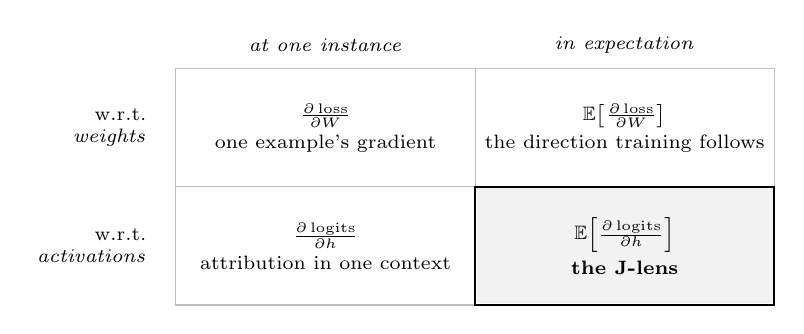
\begin{tikzpicture}[cell/.style={font=\scriptsize,align=center}]
\draw[gray!50] (0,0) rectangle (7.6,3.0);
\draw[gray!50] (3.8,0) -- (3.8,3.0);
\draw[gray!50] (0,1.5) -- (7.6,1.5);
\node[cell] at (1.9,3.3)  {\emph{at one instance}};
\node[cell] at (5.7,3.3)  {\emph{in expectation}};
\node[cell,anchor=east,align=right] at (-0.25,2.25) {w.r.t.\\ \emph{weights}};
\node[cell,anchor=east,align=right] at (-0.25,0.75) {w.r.t.\\ \emph{activations}};
\node[cell] at (1.9,2.25) {$\frac{\partial\,\mathrm{loss}}{\partial W}$\\[2pt] one example's gradient};
\node[cell] at (5.7,2.25) {$\mathbb{E}\!\left[\frac{\partial\,\mathrm{loss}}{\partial W}\right]$\\[2pt] the direction training follows};
\node[cell] at (1.9,0.75) {$\frac{\partial\,\logits}{\partial h}$\\[2pt] attribution in one context};
\fill[gray!10] (3.82,0.02) rectangle (7.58,1.48);
\node[cell] at (5.7,0.75) {$\mathbb{E}\!\left[\frac{\partial\,\logits}{\partial h}\right]$\\[2pt] \textbf{the J-lens}};
\draw[thick] (3.8,0) rectangle (7.6,1.5);
\end{tikzpicture}
\caption{Four derivative objects from the same contract. The top row has always steered \emph{training}; the bottom-left explains single predictions after the fact. The fourth square---activation Jacobians taken \emph{in expectation}---is the new instrument.}
\label{fig:four-square}
\end{figure}


Specifically, the \textbf{J-lens} is an expected derivative of \textit{logits}---scores given by the model to the tokens (word fragments) at its disposal for sampling next---with respect to \textit{activations}---the forward-propagating internal states of the model. It is a matrix, where each \(v\)-th row represents the logit index for token \(v\) in the vocabulary, and each \(d\)-th column of row \(v\) denotes the influence of activation dimension \(d\) on that \(v\)-th token. Figure~\ref{fig:jlens-rows} articulates the shape and nature of the object. Being a derivative object, it doesn't give us static data about what the activations \textit{stand for}, but instead where they \textit{point}. This matrix can then attribute disposition---in terms of propensity toward \textit{tokens}, which are proxies for \textit{concepts}---to the heretofore inscrutable latent space of the model. 


%% What a row of the J-lens is: one token's sensitivity to every activation coordinate.
%% Reference as Figure~\ref{fig:jlens-rows}.
\begin{figure}[htbp]
\centering
\resizebox{0.92\textwidth}{!}{%
\begin{tikzpicture}
% ---- the activation: a column vector, one entry per model dimension
\node[jlab] at (0,2.62) {an activation $h$};
\foreach \Y/\txt/\col in {2.00/$x$/jtea, 1.50/$y$/jorg, 1.00/$\vdots$/black, 0.50/$z$/jvio}{
  \node[jlab,\col] at (0,\Y) {\txt};}
\draw (-0.30,2.25) -| (-0.42,0.25) -- (-0.30,0.25);
\draw ( 0.30,2.25) -| ( 0.42,0.25) -- ( 0.30,0.25);
\foreach \Y/\ix in {2.00/0, 1.50/1, 1.00/$\vdots$, 0.50/{$\dmodel\!-\!1$}}{
  \node[jlabS,gray!70!black,anchor=east] at (-0.60,\Y) {\ix};}
\node[jlabS,gray!70!black,anchor=west] at (0.60,1.25) {\emph{one entry per dimension}};
% ---- the J-lens MATRIX: one row per token in the vocabulary; two of them named
\draw[thick] (-4.92,-0.42) -- (-5.12,-0.42) -- (-5.12,-3.68) -- (-4.92,-3.68);
\draw[thick] ( 4.92,-0.42) -- ( 5.12,-0.42) -- ( 5.12,-3.68) -- ( 4.92,-3.68);
\node[jlab] at (-6.05,-2.05) {$\jlens$};
\node[jlabS,gray!70!black,align=center] at (-6.05,-2.62) {one row\\ per token};
\foreach \RY/\tok in {-1.05/dog, -3.05/est}{
  \foreach \X in {-3.85,-1.28,3.85}{
    \draw[thick,fill=gray!8] (\X-1.10,\RY-0.48) rectangle (\X+1.10,\RY+0.48);}
  \node[jlab] at (1.28,\RY) {$\cdots$};
  \node[jlab,anchor=west] at (5.32,\RY) {row for ``\texttt{\tok}''};}
% the rest of the vocabulary's rows, elided
\foreach \X in {-3.85,-1.28,3.85}{\node[jlab] at (\X,-2.05) {$\vdots$};}
\node[jlab] at (1.28,-2.05) {$\ddots$};
% ---- what sits in each cell: the partial of that token's logit w.r.t. that coordinate
\foreach \X/\den/\col in {-3.85/x/jtea, -1.28/y/jorg, 3.85/z/jvio}{
  \node[jlabS] at (\X,-1.05) {$\mathbb{E}\!\left[\dfrac{\partial\,\text{``\texttt{dog}''}}{\partial {\color{\col}\den}}\right]$};
  \node[jlabS] at (\X,-3.05) {$\mathbb{E}\!\left[\dfrac{\partial\,\text{``\texttt{est}''}}{\partial {\color{\col}\den}}\right]$};}
% ---- tie the two objects together
\draw[gray!55,thin,dashed] (-0.42,0.25) to[out=-140,in=60] (-3.85,-0.62);
\node[jlabS,gray!70!black,align=center] at (0,-4.05)
  {one cell per activation coordinate: \emph{how hard that coordinate pushes on that token}};
\end{tikzpicture}}
% CAPTION STUB (Ben to expand)
\caption{What the rows of the \textbf{J-lens} are. An activation $h$ carries one number per model dimension (left, indexed $0 \dots \dmodel\!-\!1$). The \textbf{J-lens} holds one \emph{row} per token in the vocabulary, and that row holds one entry per activation coordinate: the \emph{expected} derivative of that token's logit with respect to that coordinate---averaged, as every entry here is, over the contexts and positions the lens was fit on. Reading across the ``\texttt{dog}'' row tells us how each direction of $h$ pushes the model toward saying \emph{dog}; the ``\texttt{est}'' row says the same for \emph{est}. The matrix is thus $|V| \times \dmodel$---as many rows as there are tokens to say, as many columns as there are dimensions to say them with.}
\label{fig:jlens-rows}
\end{figure}

It is important to impress that the \textbf{J-lens} doesn't just \textit{correlate} internal activations with external verbalization potentials. The \textbf{J-lens} is only statistical to the extent that it is the product of \textit{averaging} many precisely correct values. It does not offer a merely post-hoc, explanatory picture of interpretability, where statements can be made to the effect of: ``this circuit of neurons tends to fire when the model discusses dogs, so therefore this circuit may encode something about dogs.'' These networks (when trained) are entirely deterministic and static; these Jacobians speak only the language of analytically-derived \textit{cause}. They allow us to say: ``this bundle of activated neurons reflects that the model is disposed to mention dogs; if we amplify these currently-activated neurons, the model \textit{will} mention dogs more.''

Further, once the directions in the model's activation space are inflected conceptually, we can do better than just \textit{identify} disposition implied by state. We can tap the tools from the abstract formalism of linear algebra to work---observe, illustratively decompose, perturb, and steer---in a now-interpretable space with economy. Cue the \textbf{J-space}. The \textbf{J-lens} gives us white light---potent, but over-saturated and noisy. The \textbf{J-space} is a prism fit on this light, in the form of a linear decomposition. Through it, we only keep those \textbf{J-lens} directions that carry the disproportionate weight of the model's disposition as specified by the lens.\footnote{If we can expect to see anything like cognition and thoughts inside a language model, we have to hope that they can be put in the reduced terms of a few dozen---not dozens of thousands---of concepts.} The prism proves more than pretty; the \textbf{J-space} has been shown (in diverse though duly limited experiments, detailed in \S\ref{jvizllm}) as a privileged causal seat---which LLMs learned to use via training, and which we are now learning to use as well.


This document will explain the definitions and techniques employed to compute the \textbf{J-lens} and the \textbf{J-space} and will seek to elucidate how rewarding our chosen formulation for deep learning---\textit{differentiable vector spaces}---is and can continue to be. 

\section{Transformer Architecture: Positions, Layers, Logits, the Residual Stream, and Normalization}




%% A (v2.2): one column of weights, S residual streams; Anthropic index convention
\begin{figure}[htbp]
\centering
\resizebox{0.95\textwidth}{!}{%
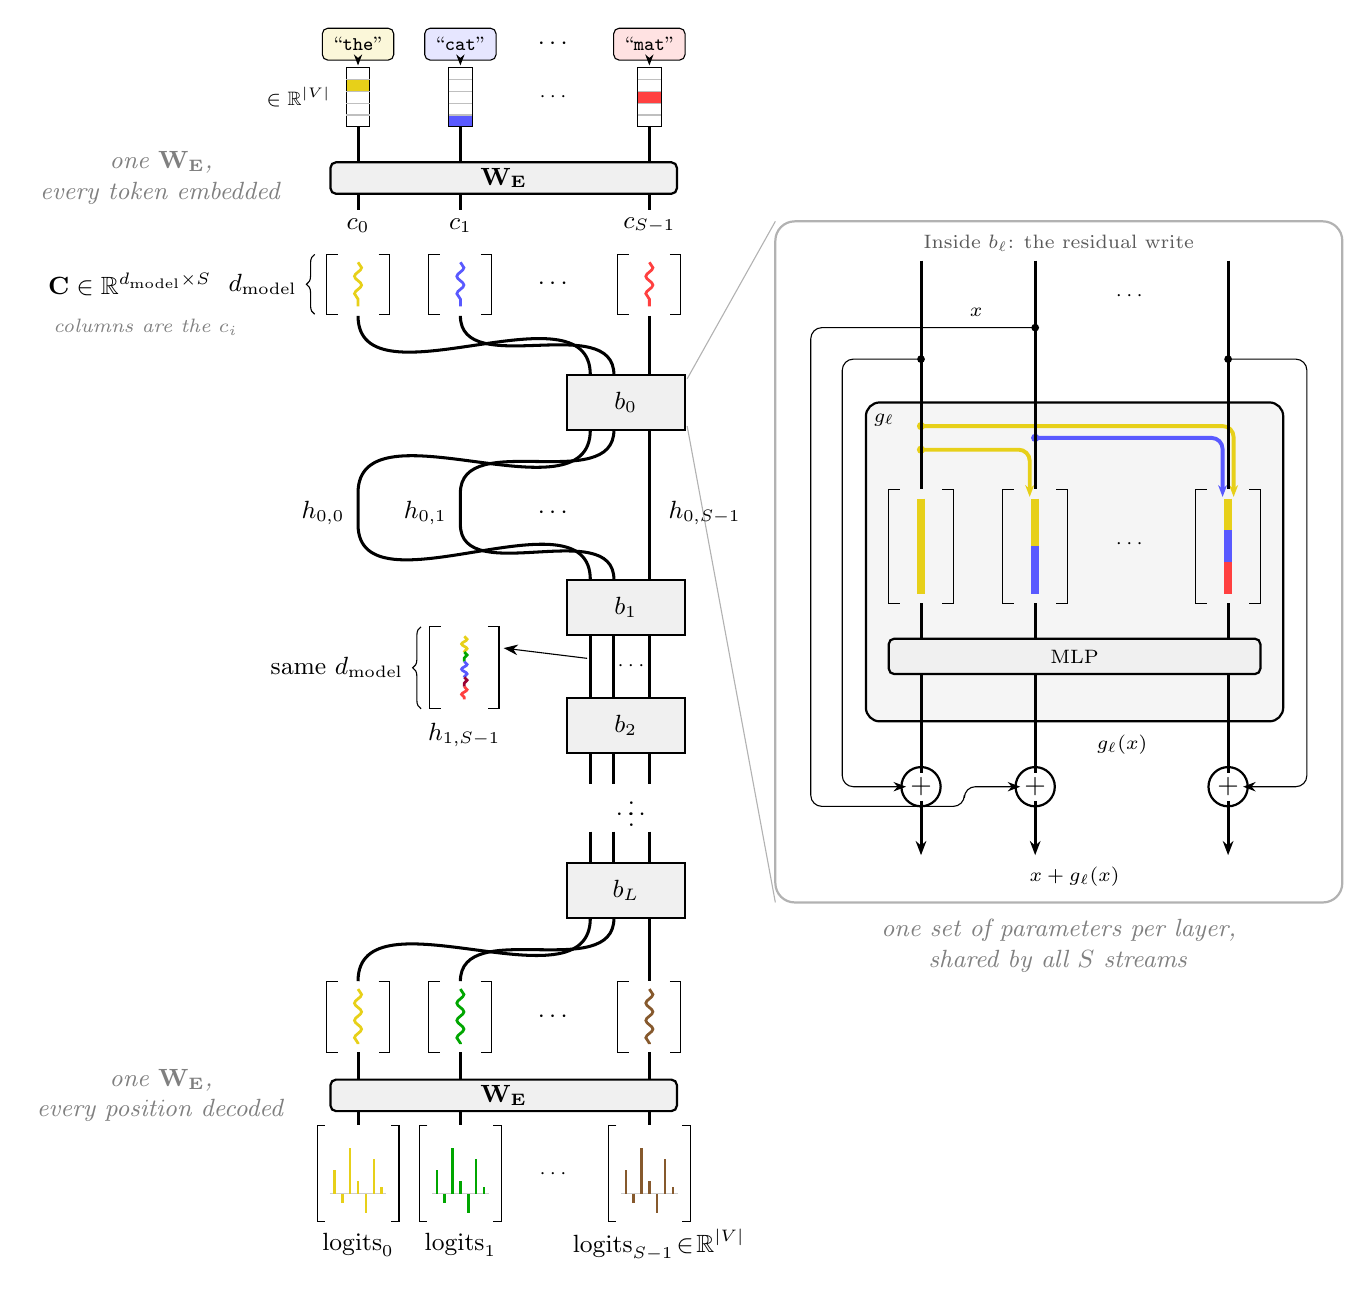
\begin{tikzpicture}
% ---- top: C matrix framing + input context vectors c_0 ... c_S
\node[jlab,align=center] at (-6.3,0.0)
      {$\mathbf{C} \in \mathbb{R}^{\dmodel \times S}$};
% \draw[-{Stealth[length=1.8mm]},gray] (-5.35,-0.15) -- (-4.35,-0.05);
\node[jlabS,gray] at (-6.1,-0.55) {\emph{columns are the $c_i$}};
\node[jlab] at (-3.4,0.75) {$c_0$}; \node[jlab] at (-2.1,0.75) {$c_1$};
\node[jlab] at (-0.9,0.0) {$\cdots$}; \node[jlab] at (0.3,0.75) {$c_{S-1}$};
\foreach \X/\tc in {-3.4/jyel,-2.1/jblu,0.3/jred}{
  \draw (\X-0.26,0.38) -| (\X-0.40,-0.38) -- (\X-0.26,-0.38);
  \draw (\X+0.26,0.38) -| (\X+0.40,-0.38) -- (\X+0.26,-0.38);
  \draw[\tc,line width=1pt,decorate,decoration={snake,amplitude=.45mm,segment length=2.2mm}]
        (\X,0.28) -- (\X,-0.28);}
\draw[decorate,decoration={brace,mirror,amplitude=3pt}] (-3.95,0.38) -- (-3.95,-0.38)
      node[midway,left=3pt,jlab]{$\dmodel$};
% ---- input embedding: text -> one-hots -> one shared W_E -> the c_i (mirror of the unembed below)
\node[draw,rounded corners=2pt,fill=jyel!15,font=\scriptsize] at (-3.4,3.05) {``\texttt{the}''};
\node[draw,rounded corners=2pt,fill=jblu!15,font=\scriptsize] at (-2.1,3.05) {``\texttt{cat}''};
\node[jlab] at (-0.9,3.05) {$\cdots$};
\node[draw,rounded corners=2pt,fill=jred!15,font=\scriptsize] at (0.3,3.05) {``\texttt{mat}''};
\foreach \X/\vc/\fy in {-3.4/jyel/2.60,-2.1/jblu/2.15,0.3/jred/2.45}{
  \fill[\vc] (\X-0.15,\fy) rectangle (\X+0.15,\fy-0.15);
  \draw (\X-0.15,2.75) rectangle (\X+0.15,2.0);
  \foreach \yy in {2.60,2.45,2.30,2.15}{\draw[gray!50] (\X-0.15,\yy) -- (\X+0.15,\yy);}}
\node[jlabS] at (-0.9,2.375) {$\cdots$};
\node[jlabS,left] at (-3.62,2.375) {$\in\mathbb{R}^{|V|}$};
\draw[thick,fill=gray!12,rounded corners=2pt] (-3.75,1.15) rectangle (0.65,1.55);
\node[font=\small] at (-1.55,1.35) {\(\mathbf{W_E}\)};
\foreach \X in {-3.4,-2.1,0.3}{
  \draw[-{Stealth[length=1.4mm]}] (\X,2.88) -- (\X,2.78);
  \draw[jresid] (\X,2.0) -- (\X,1.55);
  \draw[jresid] (\X,1.15) -- (\X,0.95);}
\node[jlab,gray,align=center] at (-5.9,1.35) {\emph{one \(\mathbf{W_E}\),}\\ \emph{every token embedded}};
% ---- the single stack of blocks (ONE set of weights per layer)
\node[jblock] (b0) at (0,-1.5) {$b_0$};
\node[jblock] (b1) at (0,-4.1) {$b_1$};
\node[jblock] (b2) at (0,-5.6) {$b_2$};
\node[jblock] (bL) at (0,-7.7) {$b_L$};
% ---- streams into b_0
\draw[jresid] (-3.4,-0.40) to[out=-90,in=90] (-0.45,-1.15);
\draw[jresid] (-2.1,-0.40) to[out=-90,in=90] (-0.15,-1.15);
\draw[jresid] (0.3,-0.40) -- (0.3,-1.15);
% ---- ONE big cutaway of b_0: the residual write, with attention seen happening inside g_ell
% connector: b_0 -> the window (spans its full height)
\draw[gray!60,thin] (0.78,-1.2) -- (1.9,0.8);
\draw[gray!60,thin] (0.78,-1.8) -- (1.9,-7.85);
% ===== the window: inside b_ell, the residual write, ALL S streams =====
% Every position has its own cord, its own split, its own sum. g_ell is ONE shared
% compound (attn + MLP) that all cords pass THROUGH; every bypass routes strictly
% AROUND it, outside its frame. Two crossings are unavoidable (and provably minimal):
% the middle cord's bypass must hop one neighbour on its way out and back.
\draw[rounded corners=7pt,thick,gray!60] (1.9,0.8) rectangle (9.1,-7.85);
\node[jlabS,gray!70!black] at (5.5,0.52) {Inside $b_\ell$: the residual write};
% ===== g_ell: the compound the cords pass through. Nothing else enters this frame. =====
% Cord spacing follows the figure's "|| ... |" pattern, which also puts the MLP box's
% centre in the wide gap --- so its label can sit dead centre without meeting a cord.
\draw[rounded corners=5pt,thick,fill=gray!8] (3.05,-1.50) rectangle (8.35,-5.55);
\node[jlabS] at (3.28,-1.72) {$g_\ell$};
% ---- attention, wired with cords: a coloured cord branches off each INCOMING residual
% and lands in the top of the latent it reaches. Position t's attention moves what the
% streams brought IN, not what the mixed latents already hold.
\foreach \X in {3.75,5.20,7.65}{
  \draw (\X-0.27,-2.60) -| (\X-0.41,-4.05) -- (\X-0.27,-4.05);
  \draw (\X+0.27,-2.60) -| (\X+0.41,-4.05) -- (\X+0.27,-4.05);}
\draw[jyel,line width=3pt] (3.75,-2.72) -- (3.75,-3.93);
\draw[jyel,line width=3pt] (5.20,-2.72) -- (5.20,-3.325);
\draw[jblu,line width=3pt] (5.20,-3.325) -- (5.20,-3.93);
\draw[jyel,line width=3pt] (7.65,-2.72) -- (7.65,-3.123);
\draw[jblu,line width=3pt] (7.65,-3.123) -- (7.65,-3.527);
\draw[jred,line width=3pt] (7.65,-3.527) -- (7.65,-3.93);
\node[jlabS] at (6.42,-3.30) {$\cdots$};
% farthest destination takes the outermost lane, so no two wires cross
\draw[jyel,line width=1.4pt,rounded corners=4pt,-{Stealth[length=1.5mm]}]
      (3.75,-1.80) -- (7.72,-1.80) -- (7.72,-2.70);
\draw[jblu,line width=1.4pt,rounded corners=4pt,-{Stealth[length=1.5mm]}]
      (5.20,-1.95) -- (7.58,-1.95) -- (7.58,-2.70);
\draw[jyel,line width=1.4pt,rounded corners=4pt,-{Stealth[length=1.5mm]}]
      (3.75,-2.10) -- (5.13,-2.10) -- (5.13,-2.70);
\fill[jyel] (3.75,-1.80) circle (1.5pt);
\fill[jyel] (3.75,-2.10) circle (1.5pt);
\fill[jblu] (5.20,-1.95) circle (1.5pt);
% ---- the MLP: one shared box, every position through it on its own cord
% (mirrors the W_E / W_U bottlenecks of the network at large --- no cord ever meets another)
\draw[thick,fill=gray!12,rounded corners=2pt] (3.34,-4.95) rectangle (8.06,-4.50);
\node[font=\scriptsize] at (5.70,-4.725) {MLP};
% ---- the cords themselves: in at the top, through g_ell, out at the bottom
\foreach \X in {3.75,5.20,7.65}{
  \draw[jresid] (\X,0.30) -- (\X,-2.60);
  \draw[jresid] (\X,-4.05) -- (\X,-4.50);
  \draw[jresid] (\X,-4.95) -- (\X,-6.20);}
\node[jlabS] at (6.42,-0.15) {$\cdots$};
% ---- each stream's bypass carries x AROUND the whole compound, in its own lane
% outer cords peel off to their own side; the middle one routes out past its neighbour
\draw[thin,rounded corners=4pt,-{Stealth[length=1.6mm]}]
      (3.75,-0.95) -- (2.75,-0.95) -- (2.75,-6.38) -- (3.56,-6.38);
\draw[thin,rounded corners=4pt,-{Stealth[length=1.6mm]}]
      (7.65,-0.95) -- (8.65,-0.95) -- (8.65,-6.38) -- (7.84,-6.38);
\draw[thin,rounded corners=4pt,-{Stealth[length=1.6mm]}]
      (5.20,-0.55) -- (2.35,-0.55) -- (2.35,-6.63) -- (4.30,-6.63)
                  -- (4.30,-6.38) -- (5.01,-6.38);
\foreach \X/\Y in {3.75/-0.95,5.20/-0.55,7.65/-0.95}{\fill (\X,\Y) circle (1.4pt);}
\node[jlabS] at (4.45,-0.36) {$x$};
\node[jlabS,right] at (5.86,-5.85) {$g_\ell(x)$};
% ---- every stream sums for itself
\foreach \X in {3.75,5.20,7.65}{
  \node[draw,circle,inner sep=1.4pt,thick] at (\X,-6.38) {$+$};
  \draw[jresid,-{Stealth[length=1.8mm]}] (\X,-6.56) -- (\X,-7.25);}
\node[jlabS] at (5.70,-7.52) {$x + g_\ell(x)$};
% ---- after b_0: pull the streams out and NAME them (they are the positions)
\draw[jresid] (-0.45,-1.85) to[out=-90,in=90] (-3.4,-2.65) -- (-3.4,-3.05)
              to[out=-90,in=90] (-0.45,-3.75);
\draw[jresid] (-0.15,-1.85) to[out=-90,in=90] (-2.1,-2.65) -- (-2.1,-3.05)
              to[out=-90,in=90] (-0.15,-3.75);
\draw[jresid] (0.3,-1.85) -- (0.3,-3.75);
\node[jlab,left]  at (-3.45,-2.9) {$h_{0,0}$};
\node[jlab,left]  at (-2.15,-2.9) {$h_{0,1}$};
\node[jlab]       at (-0.9,-2.9) {$\cdots$};
\node[jlab,right] at (0.42,-2.9)  {$h_{0,S-1}$};
% ---- after b_1: tap with full d_model vector (shape preserved)
\draw[jresid] (-0.45,-4.45) -- (-0.45,-5.25);
\draw[jresid] (-0.15,-4.45) -- (-0.15,-5.25);
\draw[jresid] (0.3,-4.45) -- (0.3,-5.25);
\node[jlabS] at (0.090,-4.85) {$\cdots$};
\draw[-{Stealth[length=1.8mm]}] (-0.49,-4.75) -- (-1.55,-4.62);
\draw (-2.35,-4.35) -| (-2.49,-5.39) -- (-2.35,-5.39);
\draw (-1.75,-4.35) -| (-1.61,-5.39) -- (-1.75,-5.39);
% h_{1,S-1}: the three content colors, one layer in --- beginning to mix (soft-blended borders)
\draw[jyel,line width=1pt,decorate,decoration={snake,amplitude=.35mm,segment length=1.2mm}] (-2.05,-4.47) -- (-2.05,-4.67);
\draw[jmixYB,line width=1pt,decorate,decoration={snake,amplitude=.35mm,segment length=1.2mm}] (-2.05,-4.67) -- (-2.05,-4.79);
\draw[jblu,line width=1pt,decorate,decoration={snake,amplitude=.35mm,segment length=1.2mm}] (-2.05,-4.79) -- (-2.05,-4.99);
\draw[jmixBR,line width=1pt,decorate,decoration={snake,amplitude=.35mm,segment length=1.2mm}] (-2.05,-4.99) -- (-2.05,-5.11);
\draw[jred,line width=1pt,decorate,decoration={snake,amplitude=.35mm,segment length=1.2mm}] (-2.05,-5.11) -- (-2.05,-5.27);
\draw[decorate,decoration={brace,mirror,amplitude=3pt}] (-2.60,-4.35) -- (-2.60,-5.39)
      node[midway,left=3pt,jlab]{same $\dmodel$};
\node[jlab] at (-2.05,-5.72) {$h_{1,S-1}$};
% ---- bundled cords downward
\draw[jresid] (-0.45,-5.95) -- (-0.45,-6.35);
\draw[jresid] (-0.15,-5.95) -- (-0.15,-6.35);
\draw[jresid] (0.3,-5.95) -- (0.3,-6.35);
\node[jlab] at (0.072,-6.62) {$\vdots$};
\node[jlab] at (0.09,-6.732) {$\cdots$};
\draw[jresid] (-0.45,-6.95) -- (-0.45,-7.35);
\draw[jresid] (-0.15,-6.95) -- (-0.15,-7.35);
\draw[jresid] (0.3,-6.95) -- (0.3,-7.35);
% ---- the point, stated on-figure
\node[jlab,gray,align=center] at (5.5,-8.4)
      {\emph{one set of parameters per layer,}\\ \emph{shared by all $S$ streams}};
% (the residual write is ONE cutaway off b_0, above; attention is seen inside its g_ell box)
% ---- bottom: fan back out; unembed only the final stream
\draw[jresid] (-0.45,-8.05) to[out=-90,in=90] (-3.4,-8.85);
\draw[jresid] (-0.15,-8.05) to[out=-90,in=90] (-2.1,-8.85);
\draw[jresid] (0.3,-8.05) -- (0.3,-8.85);
% final latents, fully mixed: h_{L,0} pure yellow, h_{L,1} green (Y+B), h_{L,S-1} brown (Y+B+R)
\foreach \X/\vc in {-3.4/jyel,-2.1/jmixYB,0.3/jmixYBR}{
  \draw (\X-0.26,-8.85) -| (\X-0.40,-9.75) -- (\X-0.26,-9.75);
  \draw (\X+0.26,-8.85) -| (\X+0.40,-9.75) -- (\X+0.26,-9.75);
  \draw[\vc,line width=1pt,decorate,decoration={snake,amplitude=.45mm,segment length=2.2mm}]
        (\X,-8.95) -- (\X,-9.65);}
\node[jlab] at (-0.9,-9.3) {$\cdots$};
% ---- unembed EVERY final stream through one shared W_U (mirror of W_E at top)
\draw[jresid] (-3.4,-9.75) -- (-3.4,-10.1);
\draw[jresid] (-2.1,-9.75) -- (-2.1,-10.1);
\draw[jresid] (0.3,-9.75) -- (0.3,-10.1);
\draw[thick,fill=gray!12,rounded corners=2pt] (-3.75,-10.5) rectangle (0.65,-10.1);
\node[font=\small] at (-1.55,-10.3) {\(\mathbf{W_E}\)};
\draw[jresid] (-3.4,-10.5) -- (-3.4,-10.68);
\draw[jresid] (-2.1,-10.5) -- (-2.1,-10.68);
\draw[jresid] (0.3,-10.5) -- (0.3,-10.68);
\foreach \X/\vc in {-3.4/jyel,-2.1/jmixYB,0.3/jmixYBR}{
  \draw (\X-0.42,-10.68) -| (\X-0.52,-11.9) -- (\X-0.42,-11.9);
  \draw (\X+0.42,-10.68) -| (\X+0.52,-11.9) -- (\X+0.42,-11.9);
  \draw[gray!40,thin] (\X-0.36,-11.55) -- (\X+0.36,-11.55);
  \foreach \i/\v in {0/0.30,1/-0.12,2/0.58,3/0.16,4/-0.24,5/0.44,6/0.09}{
    \draw[\vc,line width=0.9pt] (\X-0.3+\i*0.1,-11.55) -- ++(0,\v);}}
\node[jlabS] at (-0.9,-11.3) {$\cdots$};
\node[jlab] at (-3.4,-12.2) {$\logits_0$};
\node[jlab] at (-2.1,-12.2) {$\logits_1$};
\node[jlab] at (0.42,-12.2) {$\logits_{S-1}\!\in\!\mathbb{R}^{|V|}$};
\node[jlab,gray,align=center] at (-5.9,-10.3) {\emph{one \(\mathbf{W_E}\),}\\ \emph{every position decoded}};
\end{tikzpicture}}
% CAPTION STUB (Ben to expand): the old long caption was trimmed at Ben's request.
\caption{The transformer as one stack of blocks $b_\ell$ and $S$ residual stream cords. Tokens enter as text, become one-hots, and are mapped by a single shared \(\mathbf{W_E}\) into the columns $c_i$ of $\mathbf{C}$ (top). The blocks carry and mix these residual states through depth. Every final latent is decoded by a single shared \(\mathbf{W_E}\) into its logits (bottom). Colors trace content---each token enters in its own hue, attention \emph{moves} it across positions, and depth \emph{mixes} the bands into the final blended states.}
\label{fig:transformer-grid}
\end{figure}



To appreciate the \textbf{J-lens} and the \textbf{J-space}, a review of some principal features of the \textbf{Transformer} neural network architecture (that which carries out most modern LLMs) is in order. The key elements we'll discuss are:

\begin{enumerate}
    \item The manner in which token \textbf{Position} is represented and handled in the transformer's computation
    \item The way computation propagates forward through the \textbf{Layers} of the network
    \item The key output of the network which represents its prediction for best choice of \textit{next} token, the non-normalized vector of \textbf{Logits}
    \item The cord which carries \textit{state} through the layers of the model, the \textbf{Residual Stream}
    \item \textbf{Normalization} as a mechanism of abstraction in spatial representation
\end{enumerate}

At a high level, the transformer takes as input a context matrix, \(\mathbf{C}\), where each column, \(c_i\), represents a token of input as a vector.\footnote{This explanation of transformers ignores tokenization, one-hot representation, and embeddings and jumps right to contexts as being already embedded. Figure~\ref{fig:transformer-grid} hints at the tokenization and embedding stages, but they are less pertinent to the \textbf{J-lens} and \textbf{J-space}.} The transformer admits any sequence length, \(S\), meaning \(\mathbf{C}\)'s column count is \textit{free}. The dimension of each \(c_i\), though, is fixed model-wide at \(\dmodel\). The network's weights contract against \(\dmodel\), so \(S\) naturally carries forward seamlessly through each layer.

Strictly speaking, the transformer computes \(S\) final activation vectors, \(h_{L, t}\), for all \(t < S\).\footnote{A note on subscripts, used throughout: the first indexes the \textit{layer boundary}---\(h_{\ell, t}\) is the residual state at position \(t\) just after block \(b_\ell\), with \(L\) reserved for the final layer---and the second indexes the \textit{position}. At various points in the document, either subscript will be omitted when it doesn't detract from what is being explained; if there is only one subscript, it corresponds to \textit{layer}.} Though it is performed on all final activations during training, once the model is trained and ready to be used for autoregressive \textit{generation}, only the final activation \(h_{L, S-1}\) is decoded via an \textit{un}embedding matrix, \(\mathbf{W_U} \in \mathbb{R}^{|V| \times \dmodel}\), where \(V\) is the token vocabulary and \(|V|\) its size. This decoding produces a vector, \(\logits_{S-1} \in \mathbb{R}^{|V|}\), representing the raw weight assigned to every possible token in the vocabulary as a candidate to come \textit{next} in the sequence. \(\logits_{S-1}\) itself is not a probability distribution---it still awaits normalization via the \(\smax\) function---but it is its direct proxy, as Softmax maintains order. Once we turn \(\logits_{S-1}\) into a probability distribution via \(\smax\), we can sample the distribution, choose a new token, and create a new context matrix $\mathbf{C} \in \mathbb{R}^{\dmodel \times (S+1)}$ where \(c_S\) is the vector representation of the new token, and repeat. 

\subsection{Positions}

In autoregressive generation only the final position's logits are decoded into the next token, though tokens at all positions must be fed into the model for any forward pass. Correspondingly, logits are produced at \textit{every} position---in fact, during training, every position's logits receive a loss. Why include every prior position? The transformer architecture is such that each latent \(h_{\ell, t}\) is informed by all of the tokens at positions \(i\le t\). In each transformer block, \(b_\ell\), there is a module known as an \textbf{Attention Mechanism}, which facilitates the flow of information from the previous boundary's latents \(h_{\ell-1, i}\) into \(h_{\ell, t}\), for all positions \(i \le t\). Figure~\ref{fig:transformer-grid} articulates this information flow at a high level.

This forward-only flow of contextual information along the token axis is a vital element of the construction of the \textbf{J-lens}. Though \(\logits_{S-1}\) is produced by decoding only \(h_{L, S-1}\) directly, attention makes it such that a latent \(h_{\ell, t}\) at any layer and position has a causal impact on \(\logits_{S-1}\).\footnote{With one notable exception: final-layer latents at non-final positions, \(h_{L, t}\) with \(i < S-1\), are causal dead ends for \(\logits_{S-1}\), since no attention remains downstream of them to carry their contents across streams.} 

The goal for the \textbf{J-lens} is to formalize a general relationship between any latent and all downstream logits, on average. This is precisely what enables it to inform \textit{general verbalizable disposition}, as opposed to a more constrained quantity only pertaining to the logits at any latent's own position. \S\ref{sec:jcomp} covers the precise mechanism in more detail, but in computing the \textbf{J-lens}, we take Jacobians and average them over both directions of the position axis, pairing every source latent \(h_{\ell,t}\) with every logit vector it feeds, \(\logits_{t'}\) for \(t' \ge t\).\footnote{For a context of \(S=100\) tokens, that is \(100 + 99 + \cdots + 1 = 5050\) Jacobians per layer. \(h_{\ell,0}\) contributes one Jacobian for the 100 downstream logit vectors, and \(\logits_{99}\) receives one from each of the 100 latents in layer \(\ell\) that inform it. Furthermore, beyond just averaging Jacobians over token positions within a single context, the \textbf{J-lens} also averages them across contexts.} The payoff is that each layer's \textbf{J-lens} $\jlens_\ell$, once computed, is not bound by position at all---we get one \(\mathbf{W_U}\)-shaped map, applicable to any latent in the stream at layer $\ell$. 

\subsection{Layers}

\begin{figure}[htbp]
\centering
\resizebox{0.72\textwidth}{!}{%
\begin{tikzpicture}
% ---- nested transports R_ell (h_ell -> h_L): F stripped of the readout,
%      confined to the residual column, stopping at h_L (never reaching W_U)
\draw[rounded corners=7pt,teal!45,fill=teal!6] (-1.60,-0.85) rectangle (1.60,-8.75);
\draw[rounded corners=7pt,teal!57,fill=teal!11] (-1.15,-3.6) rectangle (1.20,-8.75);
\draw[rounded corners=7pt,teal!68,fill=teal!17] (-0.70,-5.75) rectangle (0.90,-8.75);
% ---- input vector h_ell
\draw (-0.30,0.5) -| (-0.44,-0.5) -- (-0.30,-0.5);
\draw (0.30,0.5) -| (0.44,-0.5) -- (0.30,-0.5);
\draw[decorate,decoration={snake,amplitude=.45mm,segment length=2.2mm}] (0,0.38)--(0,-0.38);
\node[jlab,right] at (0.55,0) {$h_\ell$};
% ---- main column blocks
\node[jblock] (fa) at (0,-1.6) {$b_{\ell+1}$};
\draw (-0.24,-2.75) -| (-0.36,-3.35) -- (-0.24,-3.35);
\draw (0.24,-2.75) -| (0.36,-3.35) -- (0.24,-3.35);
\draw[decorate,decoration={snake,amplitude=.35mm,segment length=2mm}] (0,-2.83) -- (0,-3.27);
\node[jlab,right] at (0.5,-3.05) {$h_{\ell+1}$};
\node[jblock] (fb) at (0,-4.4) {$b_{\ell+2}$};
\node[jlab] at (0,-5.45) {$\vdots$};
\node[jblock] (fL) at (0,-6.5) {$b_L$};
\draw (-0.30,-7.55) -| (-0.44,-8.55) -- (-0.30,-8.55);
\draw (0.30,-7.55) -| (0.44,-8.55) -- (0.30,-8.55);
\draw[decorate,decoration={snake,amplitude=.45mm,segment length=2.2mm}] (0,-7.67)--(0,-8.43);
\node[jlab,below] at (0,-9.05) {$h_L$};
% ---- main residual stream
\draw[jresid] (0,-0.5)--(fa.north); \draw[jresid] (fa.south)--(0,-2.75);
\draw[jresid] (0,-3.35)--(fb.north); \draw[jresid] (fb.south)--(0,-5.1);
\draw[jresid] (0,-5.8)--(fL.north); \draw[jresid] (fL.south)--(0,-7.55);
% ---- unembedding + signed logits
\node[draw,thick,font=\small] (WU) at (2.1,-8.05) {$\mathbf{\mathbf{W_U}}$};
\draw[-{Stealth[length=2mm]},thick] (0.5,-8.05) -- (WU.west);
\begin{scope}[shift={(4.0,-8.05)}]\jlogits{0}{0}\end{scope}
\draw[-{Stealth[length=2mm]},thick] (WU.east) -- (3.2,-8.05);
\node[jlab] at (4.0,-9.15) {$\logits_{S-1}$};
% ---- nested downstream functions (bottoms clear h_L and logits)
\draw[rounded corners=9pt,thick,gray!60] (-1.85,-0.85) rectangle (5.85,-10.1);
\node[jlab,gray!60!black] at (5.35,-1.15) {$F_\ell$};
\draw[rounded corners=9pt,thick,gray!35] (-1.38,-3.6) rectangle (5.65,-9.9);
\node[jlab,gray!50] at (5.15,-3.9) {$F_{\ell+1}$};
\draw[rounded corners=9pt,thick,gray!28] (-0.92,-5.75) rectangle (5.55,-9.75);
\node[jlab,gray!50] at (4.95,-6.05) {$F_{L-1}$};
\draw[rounded corners=9pt,thick,gray!22] (1.10,-7.05) rectangle (5.45,-9.6);
\node[jlab,gray!45] at (5.0,-7.35) {$F_L$};
% ---- R transport labels
\node[jlabS,teal!52!black] at (1.30,-1.12) {$R_\ell$};
\node[jlabS,teal!60!black] at (0.88,-3.87) {$R_{\ell+1}$};
\node[jlabS,teal!68!black] at (0.56,-5.95) {$R_{L-1}$};
% ---- the family definitions: transport Jacobian and the J-lens it composes into
\node[jlab,align=left,anchor=west] at (2.35,-0.1) {$J_\ell \;\equiv\; \mathbb{E}\!\left[\frac{\partial R_\ell}{\partial h_\ell}\right]$\\[4pt] $\jlens_\ell = \mathbf{W_U}\, J_\ell \;\equiv\; \mathbb{E}\!\left[\frac{\partial F_\ell}{\partial h_\ell}\right]$};
\end{tikzpicture}}
\caption{The nested downstream functions: from $h_\ell$, everything below is $F_\ell$; one layer deeper, $F_{\ell+1}\subset F_\ell$. The \textbf{J-lens} at layer $\ell$ is the averaged differential of $F_\ell$. Note that $F_\ell$ includes $\mathbf{W_U}$: the composition lands in logit space, which is why the \textbf{J-lens} shares $\mathbf{W_U}$'s shape, $|V| \times \dmodel$. The teal bands are the \textbf{transports} $R_\ell \supset R_{\ell+1} \supset \cdots$---the same nesting stripped of the readout, each carrying its latent only as far as $h_L$ and never reaching $\mathbf{W_U}$, so each lands back in $\mathbb{R}^{\dmodel}$. The averaged differential of $R_\ell$ is the core Jacobian $J_\ell$, and $\jlens_\ell = \mathbf{W_U} J_\ell$. The innermost nests make the telescoping explicit: $F_{L-1}$ is $b_L$ followed by $\mathbf{W_U}$, and $F_L$ is nothing but $\mathbf{W_U}$ itself---there the differential is exact and context-free, and $R_L$ is the identity; the deeper the tap, the more nonlinearity the \textbf{J-lens} must average over.}
\label{fig:f-nesting}
\end{figure}


Whereas attention provisions for information to move forward along the \textit{token position} axis, a transformer's depth in \textit{layers} allows for complex, highly nonlinear processing to occur at each position. Feedforward neural networks, in general, are compositions of functions, where each layer represents another function on the output of the layers before it. When layers are given nonlinear activation functions, their composition becomes \textit{highly} nonlinear. 

At each layer of a transformer, tokens are being processed at different levels of abstraction. For idealized instance, early layers of transformers may be focused more on composing a \textit{syntactic} representation of the context, which, in later layers, is then processed for its \textit{semantic} and \textit{factual} content (syntax having been a prerequisite for anything semantic). For this reason, having a \textbf{J-lens} at every layer provides distinct insight into leverage over \(\logits_{S-1}\) at different levels of abstraction. It allows us to trace disposition through depth of representation.\footnote{In fact, Anthropic finds that the \textbf{J-space} only becomes significantly decisive in a middle band of layers.}

Further, because of the compositional nature of the transformer, the layers downstream from any specific layer, \(\ell\), can be considered a single nested function, \(F_\ell\), that maps \(h_{\ell}\) to \(\logits\) (with the rest of the context held fixed). This framing, displayed in Figure~\ref{fig:f-nesting}, becomes insightful for the purposes of computing and conceptualizing \textbf{J-lens}es. Just as usefully, we can name the purely \textit{internal} portion of this nesting. Let \(R_\ell\) be the map that carries a latent \(h_\ell\) forward through the remaining blocks to the \textit{last} latent \(h_L\): \(R_\ell(h_\ell) = h_L\). It is all of \(F_\ell\) except the final step that turns \(h_L\) into logits. Where \(F_\ell\) lands in logit space (\(\mathbb{R}^{|V|}\)), \(R_\ell\) lands right back in latent space (\(\mathbb{R}^{\dmodel}\)). The two nest in lockstep---\(R_\ell \supset R_{\ell+1} \supset \cdots\) mirroring \(F_\ell \supset F_{\ell+1} \supset \cdots\)---but no \(R_\ell\) ever reaches that final readout, and \(R_L\) is simply the identity. Figure~\ref{fig:f-nesting} draws both nestings at once. This internal map is the honest home of the network's nonlinearity, and it is what our core Jacobian will differentiate.\footnote{It is vital to notice the omission of the \textit{token position} subscript on \(h_\ell\) here. Because of attention, \(F_\ell\) requires all of the information from prior token positions. Isolating \(F\) in our minds is just a tool to represent ``the downstream network'' from a given layer.}

\subsection{Logits}

As Figure~\ref{fig:transformer-grid} and the above discussions elucidate, the transformer is trained to produce final latents, \(h_{L,t}\), at all token positions (\(t < S\)). It is simultaneously trained to fit an unembedding matrix, \(\mathbf{W_U} \in \mathbb{R}^{|V| \times \dmodel}\), which can map any of these final latents \(h_{L, t}\) to \(\logits_{t}\) vectors. Logits are the non-normalized values corresponding to each token, that are collectively fed to the \(\smax\) function to turn them into a probability distribution over tokens. In essence, \(\mathbf{W_U}\) learns a mapping from the transformer's general size for representing one token---\(\dmodel\)---to the size of the entire available vocabulary---\(|V|\). Importantly, though, \(\mathbf{W_U}\) was trained to expect that its input latent would contain contextual information pertaining to the entire prior context, already computed (i.e. it was trained to expect activations from the \textit{final layer} \(L\), not before). What we want with \textbf{J-lens}es is the ability to---in a matrix of the same \textit{shape} as \(\mathbf{W_U}\), translating across the same \textit{spaces} as \(\mathbf{W_U}\)---interpret an ``unfinished'' latent---that is, a latent at some non-final layer \(\ell < L\)---for the logits it portends. 

Prior research (the \href{https://www.lesswrong.com/posts/AcKRB8wDpdaN6v6ru/interpreting-gpt-the-logit-lens}{\textit{logit lens}}) has used \(\mathbf{W_U}\) to directly decode non-final latents into logits; while at-times insightful, this work ignores the reality of what \(\mathbf{W_U}\) has been trained to expect as input and the characteristically non-linear transformations that get us there. The \textbf{J-lens} is the principled successor to these prior methods as it faithfully differentiates back through the network, drawing a direct causal link between any latent and the ultimate logit vector it affects.


Why make the \textbf{J-lens} differentiate from logits and not from post-\(\smax\) probabilities if those probabilities are what are ultimately used to sample the next token? While \(\smax\) exaggerates the shape of the raw logit distribution, for the purposes of the \textbf{J-lens} and \textbf{J-space}---meant to quantify relative directions of disposition in the model's latents---logits will suffice without the additional derivative computation through \(\smax\).\footnote{Which, in fact, warps the confidence of the distribution, skewing the \textbf{J-lens} based on exponential confidence.} A positive causal relationship with some logit entry monotonically translates to a positive causal relationship with the corresponding token's probability of being sampled (all else being equal). 


\subsection{The Residual Stream}\label{sec:resid}
One of the key features of the transformer is its employment of \textit{residual} layers, as opposed to traditional feedforward layers. A residual layer in a neural network is a function of the form \(f(x) = x + g(x)\)---where \(g\) is the layer's actual learned transformation---rather than \(f(x) = g(x)\) outright. In essence, residual layers' weights are trained not to fully transform their inputs into outputs, but instead to compute \textit{what should be added to} their inputs to achieve some ideal output. One intuition for the plausibility of the construction is that instead of burdening the weights with the task of (\textit{a}) doing some insightful computation on \textit{x} and (\textit{b}) carrying forward the information in \textit{x} that should be kept, weights only need to learn (\textit{a}). As a direct complement to residual layers' ability to carry information \textit{forward} in the network, they also act as smooth highways for the \textit{backward} flow of gradients. The residual construction provides a kind of ballast for backward-propagating derivatives to be able to directly reach ever earlier layers without exploding or vanishing through weight matrices. Differentiating the residual form makes this plain: \(\frac{\partial f}{\partial x} = I + \frac{\partial g}{\partial x}\). Every residual layer's Jacobian is the identity plus a learned correction, so the Jacobian of an entire stack of layers is a product of near-identity factors---an unbroken causal highway from any latent to any later one. 

Residual layers have been successfully utilized before the transformer, but the transformer's entire architecture embraces the construction as first class (see Figure~\ref{fig:transformer-grid}). The \textbf{Residual \textit{Stream}} is the conventional name attributed to the additive paths that course the computational graph of the transformer. Transformer blocks are typically referred to as ``reading from'' and ``writing to'' the residual stream, connoting the stream itself as a kind of progressive \textit{state} of the network. Of course, you could interpret values passing from layer-to-layer of any non-residual network as representations of state, but when the entire network is emphatically trained on the residual paradigm, these residual vectors can more faithfully be understood as more than mere ``intermediate'' representations. They don't just happen to look like stateful highways---training actively optimizes towards this construction.

In keeping with the conventions mentioned above, \textbf{J-lens}es tie causal links from logits back to \textit{residual} activations---i.e. vectors at different spots in the residual stream. They, more than intermediate vectors \textit{within} blocks, naturally represent states in the network's forward pass. The \textbf{J-lens} then gives us interventional and observational insights into \textit{what the model has the propensity to do} given its progressive states.


\subsection{Normalization}

Transformers, as we've seen, carry state forward via the residual stream. Latents are read into blocks, where they're transformed with tensor operations---most of which are dot products---and written back to the stream for the next layer. Within blocks, these vectors are copiously normalized,\footnote{Either at the beginning of blocks, at the end, or both, depending on implementation.} stripped of their excess magnitude and kept for just the \textit{direction} they point in space (or, equivalently, the \textit{angles} they represent along the axes of high-dimensional spheres). 

Why normalize? Why \textit{direction} over precise \textit{location}? For one thing, rampant normalization makes training much smoother as the magnitude of gradients---the strings by which we puppeteer parameters into proper settings---are kept always within a tamed range. Data becomes relative, not absolute and parameters become decision-makers, not reinforcers. There are several interpretations for \textit{vectors}. As \textit{points}, they can represent locations and their differences are lengths or distances. As \textit{arrows}, they can represent directions and their differences are angles. Both angles and lengths can represent with specificity, but angles come ``out of the box'' with several distinct advantages for the purposes of deep networks. 

For systems we want to be generally decisive, capable of abstraction, and resistant to over-fitting memorization, direction and angle are a natural choice over location and distance. The former is \textit{bounded, signed, }and\textit{ scale-free}. It represents \textit{qualities} quantitatively, the exact mission of networks that we want to work in the space of concepts and categories. \textit{Alignment, indifference, }and\textit{ opposition} are the language of the normalized dot product as +1, 0, and $-1$, respectively.\footnote{\textit{Normalized} dot products, not dot products in general. Without normalization, direction and magnitude are conflated, allowing two vectors to score high in a dot product because of either true alignment or just a large length.} How can you express these notions with location and distance? 

% NOTE: "dual normalization" = the interior read-norms (inside J_ell, differentiated
% through) + the final norm applied OUTSIDE J before \mathbf{W_U} in lens = softmax(\mathbf{W_U} norm(J h)).
% (softmax is a third, read-off normalization, not differentiated -- see Logits subsec.)
% Good place to forward-ref the seam; this sentence is where the rewrite pays off.
\(\jlens\) and \(\jspace\) are fundamentally about direction and alignment. As we'll see in \S\ref{sec:jspace}, states in \(h\)-space are more decisively decomposed into their \textit{distinct} concepts---(near-)orthogonal directions are the only way to represent this notion. 

In the architectural hyperparameters of a network, we can \textit{declare} what training will \textit{instill} as first-class paradigms for computation. We did this with the residual stream and we continue it with normalization. Normalization of vectors on their way in and of residual adjustments on their way out of blocks enables the \textit{directional} paradigm to become a privileged logic in the transformer's computation. In fact, the paradigms of residuals and normalization go hand in hand. Understanding representation as arrows, the \textit{additions} that blocks make to the residual stream become angular nudges after the normalization that starts off every next block. \(b_\ell\) adds a nudge-vector to the tail of \(h_\ell\), and \(b_{\ell+1}\) immediately grabs the hypotenuse and shrinks it back to standard size, realizing \(b_\ell(h_{\ell-1})\) as a \textit{rotation} before adding its own.

Wait, if the additions contributed by residual layers are only fully realized as rotations in the \textit{subsequent} layer, does this undermine the notion that a latent vector in the residual stream \(h_\ell\) represents state? In one sense, yes, it provides us due skepticism that any \(h_\ell\) is a `perfect' representation at any point.\footnote{We shouldn't have had that view in the first place, though, as opening a latent variable is by-definition seeking an unfinished value.} Recall though, the defining improvement that \(\jlens\) makes upon the \textit{logit lens}: it cuts no corners because it differentiates \textit{through} the downstream network! Reading off \(h_\ell\) directly would be mistaken; but reading it through \(\jlens_\ell\)---which accounts for the normalization in \(b_{\ell+1}\) as part of its reading---honors exactly what we want.


\section{J-lens}

%% Opening figure: the counterfactual vision the lens gives you. Reference it
%% as Figure~\ref{fig:jlens-glasses} when writing this section's prose.
\begin{figure}[htbp]
\centering
\resizebox{0.95\textwidth}{!}{%
\begin{tikzpicture}
% ---- the true latent, bottom center: what stands in front of the glasses
\draw (-0.3,0.35) -| (-0.44,-0.35) -- (-0.3,-0.35);
\draw (0.3,0.35) -| (0.44,-0.35) -- (0.3,-0.35);
\draw[decorate,decoration={snake,amplitude=.4mm,segment length=2.1mm}] (0,0.27)--(0,-0.27);
\node[jlab,right] at (0.55,0) {$h_\ell$};
% ---- the lens object: one matrix, two rows drawn out as steering directions
\draw[thick] (-0.6,-1.15) rectangle (0.6,-2.05);
\node[jlab] at (0,-2.32) {$\jlens_\ell$};
\foreach \Y in {-1.32,-1.88}{\draw[gray!60] (-0.52,\Y) -- (0.52,\Y);}
\draw[jtea,line width=1.2pt] (-0.52,-1.5) -- (0.52,-1.5);
\draw[jvio,line width=1.2pt] (-0.52,-1.7) -- (0.52,-1.7);
\node[jlabS,jtea,left] at (-0.66,-1.5) {row $j$};
\node[jlabS,jvio,right] at (0.66,-1.7) {row $k$};
% rows leave the matrix and become the tweaks
\draw[jtea,thin,-{Stealth[length=1.3mm]}] (-1.55,-1.5) to[out=180,in=-70] (-2.35,-0.05);
\draw[jvio,thin,-{Stealth[length=1.3mm]}] (1.55,-1.7) to[out=0,in=-110] (2.35,-0.05);
% ---- tweaked copies of the latent, standing in front of each lens
\draw[gray!60,dashed,thin] (-0.44,0.1) to[out=160,in=-30] (-2.25,0.85);
\draw[gray!60,dashed,thin] (0.44,0.1) to[out=20,in=210] (2.25,0.85);
\draw (-2.9,1.35) -| (-3.04,0.65) -- (-2.9,0.65);
\draw (-2.3,1.35) -| (-2.16,0.65) -- (-2.3,0.65);
\draw[decorate,decoration={snake,amplitude=.4mm,segment length=2.1mm}] (-2.6,1.27)--(-2.6,0.73);
\node[jlabS] at (-2.6,0.32) {$h_\ell + \alpha\,{\color{jtea}v_j}$};
\draw (2.3,1.35) -| (2.16,0.65) -- (2.3,0.65);
\draw (2.9,1.35) -| (3.04,0.65) -- (2.9,0.65);
\draw[decorate,decoration={snake,amplitude=.4mm,segment length=2.1mm}] (2.6,1.27)--(2.6,0.73);
\node[jlabS] at (2.6,0.32) {$h_\ell + \alpha\,{\color{jvio}v_k}$};
% ---- looking through: one matrix multiply into the glass
\draw[line width=1.3pt,-{Stealth[length=2mm]}] (-2.6,1.5) -- (-2.6,2.16);
\node[jlab,left] at (-2.74,1.82) {$\jlens_\ell$};
\draw[line width=1.3pt,-{Stealth[length=2mm]}] (2.6,1.5) -- (2.6,2.16);
\node[jlab,right] at (2.74,1.82) {$\jlens_\ell$};
% ---- the glasses
\draw[thick] (-2.6,3.6) circle (1.5);
\draw[thick] (2.6,3.6) circle (1.5);
\draw[thick] (-1.54,4.66) to[bend left=22] (1.54,4.66);
\draw[thick] (-4.08,3.3) -- (-5.15,2.65) -- (-5.32,2.36);
\draw[thick] (4.08,3.3) -- (5.15,2.65) -- (5.32,2.36);
% ---- seen IN the left glass: counterfactual logits, deltas marked (j raised)
\jbarframe{-2.6}{3.35}
\foreach \i/\v/\c in {0/0.35/black,1/-0.25/jdn,2/0.62/jdn,3/0.2/black,4/0.45/jgrn,5/0.55/black,6/0.1/black}{
  \draw[line width=0.9pt,\c] (-3.05+\i*0.15,3.35) -- ++(0,\v);}
\foreach \i/\o in {1/-0.15,2/0.7,4/-0.3}{
  \draw[gray!70] (-3.095+\i*0.15,3.35+\o) -- (-3.005+\i*0.15,3.35+\o);}
\node[jlabS,jtea] at (-2.45,3.1) {$j$};
\node[jlabS] at (-2.6,2.62) {$\logits + \alpha\,\jlens_\ell {\color{jtea}v_j}$};
% ---- seen IN the right glass: counterfactual logits (k raised)
\jbarframe{2.6}{3.35}
\foreach \i/\v/\c in {0/0.28/jdn,1/-0.15/black,2/1.0/jgrn,3/0.2/black,4/-0.3/black,5/0.48/jdn,6/0.1/black}{
  \draw[line width=0.9pt,\c] (2.15+\i*0.15,3.35) -- ++(0,\v);}
\foreach \i/\o in {0/0.35,2/0.7,5/0.55}{
  \draw[gray!70] (2.105+\i*0.15,3.35+\o) -- (2.195+\i*0.15,3.35+\o);}
\node[jlabS,jvio] at (2.45,3.1) {$k$};
\node[jlabS] at (2.6,2.62) {$\logits + \alpha\,\jlens_\ell {\color{jvio}v_k}$};
% ---- the true forward pass: up the nose, through the real network
\draw[jresid] (0,0.35) -- (0,1.32);
\node[jmini] at (0,1.6) {$b_{\ell+1}$};
\node[jlabS,gray] at (0,2.16) {$\vdots$};
\node[jmini] at (0,2.72) {$b_{L}$};
\draw[jresid] (0,3.0) -- (0,3.24);
\node[draw,thick,font=\scriptsize] at (0,3.48) {$\mathbf{W_U}$};
\draw[jresid,-{Stealth[length=1.8mm]}] (0,3.72) -- (0,5.2);
\jbarframe{0}{5.75}
\foreach \i/\v in {0/0.35,1/-0.15,2/0.7,3/0.2,4/-0.3,5/0.55,6/0.1}{
  \draw[line width=0.9pt] (-0.45+\i*0.15,5.75) -- ++(0,\v);}
\node[jlab] at (0,7.2) {$\logits$ \ \emph{(true)}};
\end{tikzpicture}}
\caption{Counterfactual vision \textit{through} the \textbf{J-lens}: without rerunning the network, we can attain approximations of where logits will go with specific nudges on \(h_\ell\). The \textbf{J-lens} enables this vision. The true state $h_\ell$ (center) earns its logits the hard way---up through every remaining block and $\mathbf{W_U}$. The flanking states are tweaked copies of $h_\ell$, each nudged along a row of the J-lens $\jlens_\ell$ itself (rows $j$ and $k$, drawn out of the matrix at bottom)---and they never run the network at all: through the glass, $\Delta\logits = \jlens_\ell\,\Delta h$, one matrix multiply. Green bars were raised by the tweak, red lowered; gray ticks mark the true heights. Each eye's tall green bar sits exactly at the token whose row it was steered with.}
\label{fig:jlens-glasses}
\end{figure}


The \textbf{J-lens} and its family are the key objects per layer that allow all of the analysis that follows. At the core of the family is \(J_\ell \in \mathbb{R}^{\dmodel \times \dmodel}\), the expected Jacobian of the final latent \(h_L\) with respect to a prior latent \(h_\ell\). 

\[J_\ell = \mathbb{E}_{t' \ge t, \mathscr{P}}\left[\frac{\partial h_{L,t'}}{\partial h_{\ell,t}}\right]\]

While the details of the \textit{expectation} (over token positions \(t\), over prompt corpus \(\mathscr{P}\)) will be elucidated in due course, the thrust of this object is a representation of how much some downstream final-layer latent \(h_{L,t'}\) is sensitive to an upstream latent \(h_{\ell, t}\)---where ``downstream" here refers to both of the transformer's causal axes: \textit{token position} and \textit{layer}. Setting aside token positions momentarily, we have:


\[J_\ell \;\equiv\; \mathbb{E}_{t' \ge t,\, \mathscr{P}}\!\left[\frac{\partial R_\ell}{\partial h_\ell}\right]\]

This is the core step skipped by the \textit{logit lens}---the differentiation through the nonlinear layers of the network that make a latent ready for decoding via \(\mathbf{W_U}\).\footnote{If the \textit{logit lens} used \(J_\ell \cdot h_{\ell}\) instead of just \(h_{\ell}\), it would just about be the \textbf{J-lens} \(\jlens_\ell\).} 

The natural next step to get these latents speaking about \textit{logits} is to compose \(J_\ell\) with \(\mathbf{W_U}\). This gives us the \textbf{J-lens} \(\jlens\), which shares the shape (and thus the structure of translation) with \(\mathbf{W_U} \in\mathbb{R}^{|V| \times \dmodel}\).

\[\jlens_\ell = \mathbf{W_U} \cdot J_\ell\]

This matrix represents the sensitivity of some downstream \(\logits_{t'}\) to an upstream latent \(h_{\ell, t}\). It tells us, in each row \(v\) (\(\in \mathbb{R}^{\dmodel}\)), the gradient of \(\logits_{t'}[v]\) with respect to \(h_{\ell,t}\). These rows, in essence, represent the directions we'd want to push \(h_{\ell,t}\) in order to make \(\logits_{t'}[v]\) higher (i.e. to make token \(v\) more likely to be sampled downstream). If we take activations \(h_{\ell,t}\) to be \textit{arrows denoting direction} as opposed to \textit{points denoting location}, we can then measure the \textit{alignment} between the current direction of \(h_{\ell,t}\) and that of steepest logit-increase for any token we please. This brings us to the normalized \textbf{J-lens} \(\jlens(h)\) \textit{function}.

\[\jlens_\ell(h_\ell) = \smax(\mathbf{W_U} \cdot \norm(J_\ell \cdot h_\ell))\]

This takes us from some \(h_{\ell,t}\) to a probability distribution (\(\mathbb{R}^{|V|}\)) of the model's propensity to verbalize each token downstream.\footnote{If we did not want to normalize this vector of alignment scores into a probability distribution, we'd still want to normalize \(J_\ell \cdot h_\ell\) because \(\mathbf{W_U}\) expects normalized latents, and we've explicitly taken \(J_\ell\) only through the last latent, leaving out the network's typical normalization thereof.} \(\jlens_\ell(h_\ell)[v]\) tells us the expected odds of verbalization of token \(v\), as indicated by the normalized, expected Jacobian of future latents \(h_{L,t'}\) with respect to \(h_{\ell,t}\). Figure~\ref{fig:jlens-glasses} pumps intuition about the relationships \(J_\ell\) spells out and how they can be used for counterfactual insight (then, factual interventional success). 

As the computation below will detail, any \(J_\ell\) where \(\ell < L\) is but a \textit{local linear approximation} of a relationship that is by no means linear. Further, \(J_\ell\) as we define it is an \textit{average} local linear approximation of the relationship in question. Any from the set of specific Jacobians averaged to produce a single object from this family is itself entirely accurate and complete, but only to the specific \(h_{\ell,t}\) that allowed its computation. \(R_\ell\) is (for \(\ell < L\)) by-design nonlinear, so the transformation it performs on \(h_{\ell,t}\) is \textit{dependent on} \(h_{\ell,t}\) and irreducible over \(h_{\ell}\)-space without averaging.\footnote{It bears repeating: we're not just saying that the \textit{result} \(R_\ell(h_{\ell,t})\) is dependent on \(h_{\ell,t}\)---this is the nature of any function. We're saying that the actual algorithm \(R_\ell\) behaves differently for different activations.} Now the averaging, for all the specific accuracy it sheds, makes \(J_{\ell}\) and \(\jlens_\ell\) flexible over token positions and---when further averaged over the prompt corpus \(\mathscr{P}\)---flexibly relevant across semantic contexts. 

Finally, as \S\ref{sec:jspace} will show, the \textbf{J-space} decomposition \(\jspace_{\ell}(h_\ell)\) of a latent \(h_{\ell}\) is a selection of the rows of \(\jlens_{\ell}\). Thus, \(J_{\ell}\) and \(\jlens_{\ell}\) are the prerequisite objects for \textbf{J-vision} broadly.

\subsection{Computation}\label{sec:jcomp}

Our first primitive is the Jacobian \(\frac{\partial h_{L,t'}}{\partial h_{\ell,t}} \in \mathbb{R}^{\dmodel \times \dmodel}\) for any specific \(t\) and \(t' \ge t\). This matrix is built iteratively in \(\dmodel\) steps. Having cached the activations of a forward pass, we can compute the local gradient at each layer for the specific input. In order to unambiguously represent the effective \(\mathbb{R}^{\dmodel} \to \mathbb{R}^{\dmodel}\) matrix that took \(h_{\ell,t}\) to \(h_{L,t'}\) we have to individually probe the pass in each dimension with unit vectors. When \(h_{\ell,t}\) went through this transformation in the forward pass, it collapsed and lost the information of the maps at work on it in the process through frequent weighed summation. To recover the collapsed information, we seed \(\dmodel\) forward passes from layer \(\ell\) (where each layer's ``weights" are local Jacobians, frozen at the cached activations of \(h_{\ell,t}\)'s forward pass) with each standard basis vector \(e_d\) of \(\mathbb{R}^{\dmodel}\) to get each \(d\)-th column of \(\frac{\partial h_{L,t'}}{\partial h_{\ell,t}}\).\footnote{These \(e_d\) probes could be sent forward or backward equivalently---while we discuss and display the forward route, Anthropic's released materials seeded backward passes. Either way, they traverse the frozen set of linear operators unlocked and saved in the actual full forward pass of the model and recover the exact same information.} These standard basis probes are tracer dyes through the opaque local transformation, one dye per channel. Figure~\ref{fig:two-modes} depicts this computation exactly.   

%% Reverse vs forward mode on the frozen chain: fill J row-by-row (climb)
%% or column-by-column (descend). Reference as Figure~\ref{fig:two-modes}.
\begin{figure}[htbp]
\centering
\resizebox{0.82\textwidth}{!}{%
\begin{tikzpicture}[
  jop/.style={draw,thick,fill=gray!12,minimum width=13mm,minimum height=5mm,font=\scriptsize},
  jarrO/.style={jorg,line width=1.1pt,-{Stealth[length=1.4mm]}},
  jarrT/.style={jtea,line width=1.1pt,-{Stealth[length=1.4mm]}},
]
% ==== 1 - the cached forward pass, horizontal
\node[jlabS,align=left,anchor=west] at (-7.5,1.35)
  {\textbf{1 $\cdot$ run the network once} at the real context; cache every activation\\
   (ReLU masks, attention patterns). The downstream chain \emph{freezes}.};
\draw (-7.3,0.3) -| (-7.42,-0.3) -- (-7.3,-0.3);
\draw (-6.9,0.3) -| (-6.78,-0.3) -- (-6.9,-0.3);
\draw[decorate,decoration={snake,amplitude=.35mm,segment length=2mm}] (-7.1,0.24)--(-7.1,-0.24);
\node[jlabS] at (-7.1,-0.55) {$c$};
\draw[-{Stealth[length=1.4mm]}] (-6.7,0) -- (-6.4,0);
\node[jop] at (-5.7,0) {$b_0 \cdots b_\ell$};
\draw[-{Stealth[length=1.4mm]}] (-5.0,0) -- (-4.7,0);
\draw (-4.55,0.3) -| (-4.67,-0.3) -- (-4.55,-0.3);
\draw (-4.15,0.3) -| (-4.03,-0.3) -- (-4.15,-0.3);
\draw[decorate,decoration={snake,amplitude=.35mm,segment length=2mm}] (-4.35,0.24)--(-4.35,-0.24);
\node[jlabS] at (-4.35,-0.55) {$h_\ell$};
\draw[-{Stealth[length=1.4mm]}] (-3.95,0) -- (-3.65,0);
\node[jop,minimum width=17mm] at (-2.75,0) {$b_{\ell+1} \cdots b_L$};
\draw[-{Stealth[length=1.4mm]}] (-1.85,0) -- (-1.55,0);
\node[jop] at (-0.95,0) {$\mathbf{W_U}$};
\draw[-{Stealth[length=1.4mm]}] (-0.25,0) -- (0.05,0);
\draw (0.25,0.45) -| (0.13,-0.45) -- (0.25,-0.45);
\draw (1.15,0.45) -| (1.27,-0.45) -- (1.15,-0.45);
\draw[gray!40,thin] (0.25,0) -- (1.15,0);
\foreach \i/\v in {0/0.28,1/-0.12,2/0.38,3/0.15,4/-0.2}{
  \draw[line width=0.8pt] (0.34+\i*0.17,0) -- ++(0,\v);}
\node[jlabS] at (0.7,-0.68) {$\logits$};
% inner box: R_ell, the h_ell -> h_L map
\draw[rounded corners=3pt,gray!65,thick] (-3.66,0.4) rectangle (-1.84,-0.4);
\node[jlabS,gray!70!black] at (-2.75,0.6) {$R_\ell$};
% outer box: F_ell = R_ell then \mathbf{W_U}, the frozen region
\draw[dashed,rounded corners=5pt,gray!55] (-3.9,0.92) rectangle (-0.15,-0.62);
\node[jlabS,gray!70!black] at (-0.5,0.76) {$F_\ell$};
\node[jlabS,gray!70!black,align=left,anchor=west] at (1.65,0.2)
  {frozen at $h_\ell$: a chain of\\ linear operators. $R_\ell$ is the\\ $h_\ell\!\to\!h_L$ part; $\mathbf{W_U}$ finishes $F_\ell$.};
% ==== 2 - reverse mode (left): e_v climbs THROUGH W_U^T, fills a ROW of M
\node[jlabS,align=center] at (-5.1,-1.7)
  {\textbf{2 $\cdot$ through $\mathbf{W_U}$} (all of $F_\ell$): seed in \emph{vocabulary}\\ space and climb---one \textbf{row} of $\jlens$ per pass, $|V|$ of them};
\node[jop] (r1) at (-4.3,-3.55) {$\partial b_{\ell+1}^{\!\top}$};
\node[jop] (r2) at (-4.3,-4.30) {$\partial b_{\ell+2}^{\!\top}$};
\node[jlabS,gray] at (-4.3,-4.90) {$\vdots$};
\node[jop] (r3) at (-4.3,-5.50) {$\partial b_{L}^{\!\top}$};
\node[jop] (r4) at (-4.3,-6.25) {$\mathbf{W_U}^{\!\top}$};
\draw[jarrO] (-4.3,-6.00) -- (-4.3,-5.75);
\draw[jarrO] (-4.3,-5.25) -- (-4.3,-5.10);
\draw[jarrO] (-4.3,-4.70) -- (-4.3,-4.55);
\draw[jarrO] (-4.3,-4.05) -- (-4.3,-3.80);
\draw (-4.5,-6.85) -| (-4.62,-7.55) -- (-4.5,-7.55);
\draw (-4.1,-6.85) -| (-3.98,-7.55) -- (-4.1,-7.55);
\draw[jorg,line width=2.2pt] (-4.45,-6.97) -- (-4.15,-6.97);
\node[jlabS] at (-4.3,-7.80) {$e_v$ \ {\color{gray}(at the logits end)}};
\draw[jarrO] (-4.3,-6.85) -- (-4.3,-6.50);
\draw[jorg,line width=1.1pt] (-4.3,-3.30) -- (-4.3,-2.85);
\draw[jarrO] (-4.3,-2.85) -- (-5.92,-2.85);
\draw[thick] (-6.85,-2.10) rectangle (-6.00,-3.90);
\foreach \Y in {-2.35,-2.60,-2.85,-3.10,-3.35,-3.60}{\draw[gray!55] (-6.78,\Y) -- (-6.07,\Y);}
\draw[jorg,line width=1.5pt] (-6.78,-2.85) -- (-6.07,-2.85);
\node[jlabS] at (-6.42,-4.14) {$\mathbf{W_U}J(h_\ell)$};
\node[jlabS,jorg] at (-6.42,-4.43) {row $v$};
% reverse loop: M back to the e_v seed --- the big |V|-iteration loop (through W_U^T)
\draw[gray!45,dashed,line width=0.9pt,-{Stealth[length=1.7mm]}] (-6.70,-3.90) .. controls (-7.45,-5.60) and (-6.55,-7.15) .. (-4.66,-7.22);
\node[jlabS,gray!55,align=center] at (-7.2,-6.25) {$|V|$\\ iterations};
% ==== 3 - forward mode (right): e_d descends to h_L, fills a COLUMN of the SQUARE J; one W_U gives the M column
\node[jlabS,align=center] at (1.5,-1.7)
  {\textbf{3 $\cdot$ transport only} (just $R_\ell$): stop at $h_L$---one slice\\ of the \emph{square} $J$ per pass, $\dmodel$ of them};
\draw (0.85,-2.35) -| (0.73,-2.95) -- (0.85,-2.95);
\draw (1.25,-2.35) -| (1.37,-2.95) -- (1.25,-2.95);
\draw[jtea,line width=2.2pt] (0.88,-2.86) -- (1.22,-2.86);
\node[jlabS,left] at (0.58,-2.62) {{\color{gray}(at $h_\ell$)} \ $e_d$};
\draw[jarrT] (1.05,-2.95) -- (1.05,-3.10);
\node[jop] (f1) at (1.05,-3.35) {$\partial b_{\ell+1}$};
\node[jop] (f2) at (1.05,-4.10) {$\partial b_{\ell+2}$};
\node[jlabS,gray] at (1.05,-4.70) {$\vdots$};
\node[jop] (f3) at (1.05,-5.30) {$\partial b_{L}$};
\draw[jarrT] (1.05,-3.60) -- (1.05,-3.85);
\draw[jarrT] (1.05,-4.35) -- (1.05,-4.50);
\draw[jarrT] (1.05,-4.90) -- (1.05,-5.05);
\draw[jarrT] (1.05,-5.55) to[out=-90,in=180] (1.78,-5.85);
\draw[thick] (1.85,-5.15) rectangle (3.05,-6.35);
\foreach \Xc in {2.10,2.35,2.60,2.85}{\draw[gray!55] (\Xc,-5.23) -- (\Xc,-6.27);}
\draw[jtea,line width=1.5pt] (2.85,-5.23) -- (2.85,-6.27);
\node[jlabS,align=center] at (2.62,-4.74) {$J(h_\ell)$\\ {\scriptsize$\dmodel\times\dmodel$}};
\node[jlabS,jtea] at (2.45,-6.57) {column $d$};
\draw[jarrT] (3.05,-5.75) -- (3.68,-5.75);
\node[jop,minimum width=9mm] at (4.15,-5.75) {$\mathbf{W_U}$};
\draw[jarrT] (4.62,-5.75) -- (5.28,-5.75);
\draw[thick] (5.35,-4.85) rectangle (6.20,-6.65);
\foreach \Xc in {5.60,5.85,6.10}{\draw[gray!55] (\Xc,-4.93) -- (\Xc,-6.57);}
\draw[jtea,line width=1.5pt] (6.10,-4.93) -- (6.10,-6.57);
\node[jlabS] at (5.77,-4.60) {$\mathbf{W_U}J(h_\ell)$};
\node[jlabS,jtea] at (5.77,-6.88) {column $d$};
\node[jlabS,gray!70!black,align=center] at (4.15,-6.55) {$\mathbf{W_U} J = \jlens$\\ (one matmul)};
% forward loop: J back to the e_d seed --- the smaller d_model loop, up the RIGHT (CCW); W_U-to-M sits outside it
\draw[gray!45,dashed,line width=0.9pt,-{Stealth[length=1.7mm]}] (3.02,-5.18) .. controls (3.66,-4.85) and (3.62,-3.02) .. (1.48,-2.66);
\node[jlabS,gray!55,align=center] at (4.02,-3.75) {$\dmodel$\\ iterations};
% ==== the punchline
\node[jlab,gray!70!black,align=center] at (-0.4,-8.5)
  {both land the same $\mathbf{W_U}J(h_\ell)$, and the \emph{direction} is free---a square $J$ fills in $\dmodel$ passes either way.\\ The \emph{range} is the real choice: $\mathbf{W_U}$ is static and already its own Jacobian, so keeping it in the loop only bloats it to $|V|$};
\end{tikzpicture}}
\caption{Two routes to the \textbf{J-lens} matrix $\mathbf{W_U}\,J(h_\ell)$, built here at one frozen context (before averaging into $\jlens_\ell$). One forward pass at the real context anchors everything, freezing the downstream chain into a stack of linear operators; both routes reuse that single cache. The choice that matters is \textbf{how far to differentiate}. \textbf{Through $\mathbf{W_U}$} (left) seeds a one-hot $e_v$ in vocabulary space and climbs the transposes---\emph{including} $\mathbf{W_U}^{\!\top}$---depositing one \textbf{row} of $\jlens$ per pass, and so paying $|V|$ of them. \textbf{Transport only} (right) stops at $h_L$, filling the \emph{square} transport Jacobian $J$ ($\dmodel\times\dmodel$) one slice per pass and never touching $\mathbf{W_U}$; a single matmul $\mathbf{W_U}J$ then lifts the whole of it into $\jlens$. Direction is the lesser question: a square $J$ costs $\dmodel$ passes whether filled forward from $h_\ell$ or backward from $h_L$---it is drawn forward here only to show the column filling. Range is what separates them: $\mathbf{W_U}$ is a static matrix, already its own Jacobian, so carrying it inside the loop re-derives what we already have and inflates every pass into $\mathbb{R}^{|V|}$. For $(|V|, \dmodel) = (50\text{k}, 12\text{k})$, that is the $4\times$ discount.}
\label{fig:two-modes}
\end{figure}

In a single context \(\mathbf{C}_{\mathscr{p}}\) with \(S_{\mathscr{p}} =  100\),\footnote{We fix a uniform context length (\(S_{\mathscr{p}} = 100\) throughout) for concreteness. For a corpus of differing-length contexts, weigh each context's contribution when forming \(J_\ell\) so that longer ones do not dominate the mean.} we can take an average of the \((100 + 99 + \cdots + 1 =)\) 5050 individual \(\frac{\partial h_{L,t'}}{\partial h_{\ell,t}}\) matrices, each representing a (\(h_{\ell,t}\), \(h_{L, t'}\)) pair from the context. The duality of these Jacobians is beautiful. For a single context, the \(100\) in the sum could be interpreted as the \(100\) final latents \(h_{L}\) that depend on \(h_{\ell,0}\), or the \(100\) early latents \(h_{\ell,0}, \cdots, h_{\ell,99}\) informing the singular \(h_{L,99}\). Figure~\ref{fig:context-strip} and Figure~\ref{fig:fan-out}, respectively, show this exact duality. 

\begin{figure}[htbp]
\centering
\resizebox{\textwidth}{!}{%
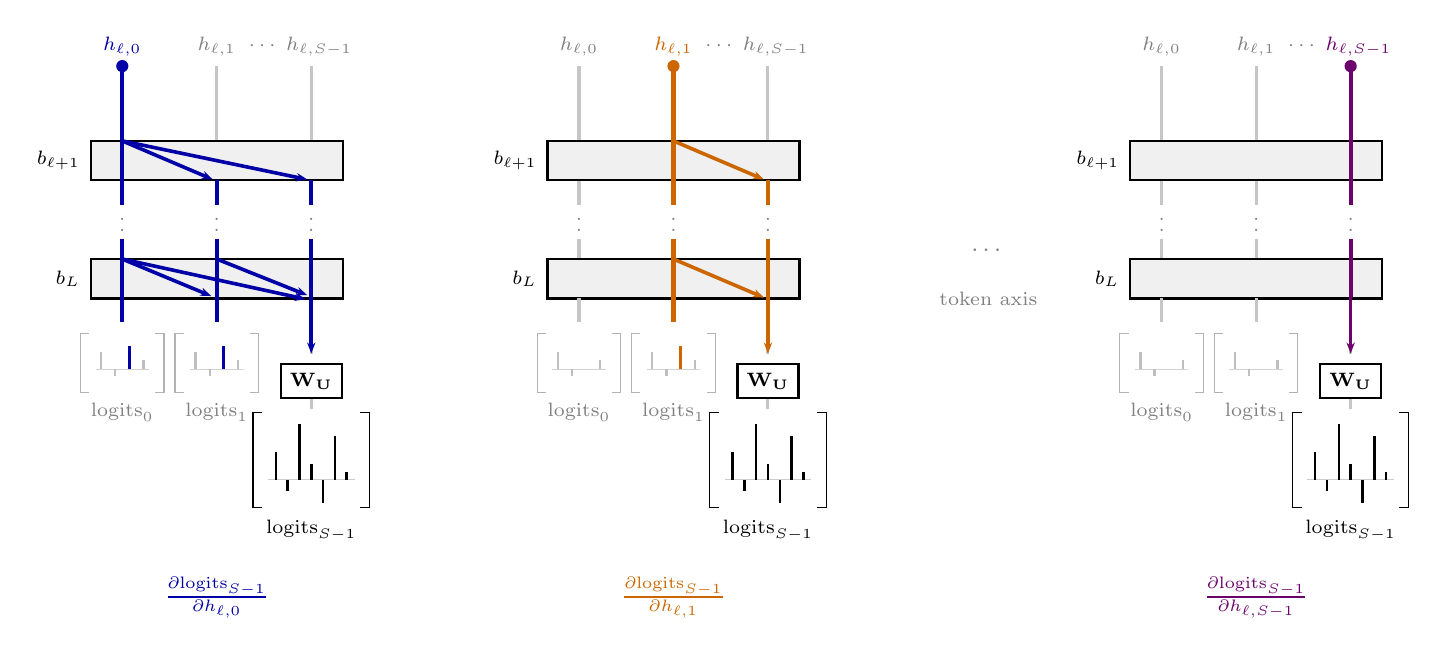
\begin{tikzpicture}[
  cord/.style={line width=1.1pt,gray!45},
  hcord/.style={line width=1.5pt,#1},
  harr/.style={line width=1.3pt,#1,-{Stealth[length=1.4mm]}},
]
%% Three panels, all happening at once: the (t, t' >= t) triangle the lens
%% averages over. Streams at x = -1.2 (pos 0), 0 (pos 1), 1.2 (pos S-1);
%% deliveries = diagonals inside blocks; vdots break every cord.
\foreach \panel/\PX in {0/0,1/5.8,2/13.2}{
\begin{scope}[xshift=\PX cm]
  \foreach \X in {-1.2,0,1.2}{
    \draw[cord] (\X,0.35) -- (\X,-0.6);
    \draw[cord] (\X,-1.1) -- (\X,-1.42);
    \node[jlabS,gray] at (\X,-1.63) {$\vdots$};
    \draw[cord] (\X,-1.84) -- (\X,-2.1);}
  \node[jlabS,gray] at (0.6,0.6) {$\cdots$};
  \node[draw,thick,fill=gray!12,minimum width=32mm,minimum height=5mm] (bA\panel) at (0,-0.85) {};
  \node[jlabS,left] at (bA\panel.west) {$b_{\ell+1}$};
  \node[draw,thick,fill=gray!12,minimum width=32mm,minimum height=5mm] (bB\panel) at (0,-2.35) {};
  \node[jlabS,left] at (bB\panel.west) {$b_{L}$};
  \draw[cord] (-1.2,-2.6) -- (-1.2,-2.9);
  \draw[cord] (0,-2.6) -- (0,-2.9);
  \draw[cord] (1.2,-2.6) -- (1.2,-3.3);
  \node[draw,thick,font=\scriptsize] (WU\panel) at (1.2,-3.65) {$\mathbf{W_U}$};
  \draw[cord] (WU\panel.south) -- (1.2,-4.0);
  \begin{scope}[shift={(1.2,-4.9)}]\jlogits{0}{0}\end{scope}
  \node[jlabS] at (1.2,-5.55) {$\logits_{S-1}$};
  % faint logits at the other positions (every stream admits unembedding)
  \foreach \mx/\mlab in {-1.2/{\logits_0},0/{\logits_1}}{
    \draw[gray!60] (\mx-0.42,-3.05) -| (\mx-0.53,-3.8) -- (\mx-0.42,-3.8);
    \draw[gray!60] (\mx+0.42,-3.05) -| (\mx+0.53,-3.8) -- (\mx+0.42,-3.8);
    \draw[gray!35,thin] (\mx-0.34,-3.5) -- (\mx+0.34,-3.5);
    \foreach \bi/\bv in {0/0.22,1/-0.09,3/0.12}{
      \draw[gray!50,line width=0.8pt] (\mx-0.27+\bi*0.18,-3.5) -- ++(0,\bv);}
    \node[jlabS,gray] at (\mx,-4.05) {$\mlab$};}
\end{scope}}
% ---- panel 1: h_{ell,0} floods every later stream and every logit
\begin{scope}
  \node[jlabS,blue!65!black] at (-1.2,0.6) {$h_{\ell,0}$};
  \node[jlabS,gray] at (0,0.6) {$h_{\ell,1}$};
  \node[jlabS,gray] at (1.3,0.6) {$h_{\ell,S-1}$};
  \fill[blue!65!black] (-1.2,0.35) circle (2.2pt);
  \draw[hcord=blue!65!black] (-1.2,0.35) -- (-1.2,-1.42);
  \draw[hcord=blue!65!black] (-1.2,-1.84) -- (-1.2,-2.6);
  \draw[hcord=blue!65!black] (-1.2,-2.6) -- (-1.2,-2.9);
  \draw[harr=blue!65!black] (-1.2,-0.6) -- (-0.05,-1.09);
  \draw[harr=blue!65!black] (-1.2,-0.6) -- (1.15,-1.09);
  \draw[hcord=blue!65!black] (0,-1.1) -- (0,-1.42);
  \draw[hcord=blue!65!black] (0,-1.84) -- (0,-2.6);
  \draw[hcord=blue!65!black] (0,-2.6) -- (0,-2.9);
  \draw[hcord=blue!65!black] (1.2,-1.1) -- (1.2,-1.42);
  \draw[hcord=blue!65!black] (1.2,-1.84) -- (1.2,-2.6);
  \draw[harr=blue!65!black] (-1.2,-2.1) -- (-0.07,-2.57);
  \draw[harr=blue!65!black] (-1.2,-2.1) -- (1.13,-2.61);
  \draw[harr=blue!65!black] (0,-2.1) -- (1.15,-2.56);
  \draw[harr=blue!65!black] (1.2,-2.6) -- (1.2,-3.3);
  \draw[blue!65!black,line width=1pt] (-1.2+0.09,-3.5) -- ++(0,0.3);
  \draw[blue!65!black,line width=1pt] (0.09,-3.5) -- ++(0,0.3);
  \node[jlab,blue!65!black] at (0,-6.4) {$\frac{\partial \logits_{S-1}}{\partial h_{\ell,0}}$};
\end{scope}
% ---- panel 2: h_{ell,1} reaches its own and later logits, never position 0
\begin{scope}[xshift=5.8cm]
  \node[jlabS,gray] at (-1.2,0.6) {$h_{\ell,0}$};
  \node[jlabS,orange!80!black] at (0,0.6) {$h_{\ell,1}$};
  \node[jlabS,gray] at (1.3,0.6) {$h_{\ell,S-1}$};
  \fill[orange!80!black] (0,0.35) circle (2.2pt);
  \draw[hcord=orange!80!black] (0,0.35) -- (0,-1.42);
  \draw[hcord=orange!80!black] (0,-1.84) -- (0,-2.6);
  \draw[hcord=orange!80!black] (0,-2.6) -- (0,-2.9);
  \draw[harr=orange!80!black] (0,-0.6) -- (1.15,-1.09);
  \draw[hcord=orange!80!black] (1.2,-1.1) -- (1.2,-1.42);
  \draw[hcord=orange!80!black] (1.2,-1.84) -- (1.2,-2.6);
  \draw[harr=orange!80!black] (0,-2.1) -- (1.15,-2.59);
  \draw[harr=orange!80!black] (1.2,-2.6) -- (1.2,-3.3);
  \draw[orange!80!black,line width=1pt] (0.09,-3.5) -- ++(0,0.3);
  \node[jlab,orange!80!black] at (0,-6.4) {$\frac{\partial \logits_{S-1}}{\partial h_{\ell,1}}$};
\end{scope}
% ---- panel 3: h_{ell,S-1}, the straight shot; only its own logits
\begin{scope}[xshift=13.2cm]
  \node[jlabS,gray] at (-1.2,0.6) {$h_{\ell,0}$};
  \node[jlabS,gray] at (0,0.6) {$h_{\ell,1}$};
  \node[jlabS,violet!85!black] at (1.3,0.6) {$h_{\ell,S-1}$};
  \fill[violet!85!black] (1.2,0.35) circle (2.2pt);
  \draw[hcord=violet!85!black] (1.2,0.35) -- (1.2,-1.42);
  \draw[hcord=violet!85!black] (1.2,-1.84) -- (1.2,-2.6);
  \draw[harr=violet!85!black] (1.2,-2.6) -- (1.2,-3.3);
  \node[jlab,violet!85!black] at (0,-6.4) {$\frac{\partial \logits_{S-1}}{\partial h_{\ell,S-1}}$};
\end{scope}
% ellipsis over the token axis, between panel 1 and panel S-1
\node[jlab,gray] at (9.8,-2.0) {$\cdots$};
\node[jlabS,gray,align=center] at (9.8,-2.6) {token axis};
\end{tikzpicture}}
\caption{This figure depicts the \textit{S} \textit{source} latents that affect the final \(\logits_{S-1}\) vector. These three panels are happening \textit{at once}. Each activation deposits some causal influence on \textit{all} logit vectors succeeding it.}
\label{fig:context-strip}
\end{figure}

\begin{figure}[htbp]
\centering
\resizebox{0.8\textwidth}{!}{%
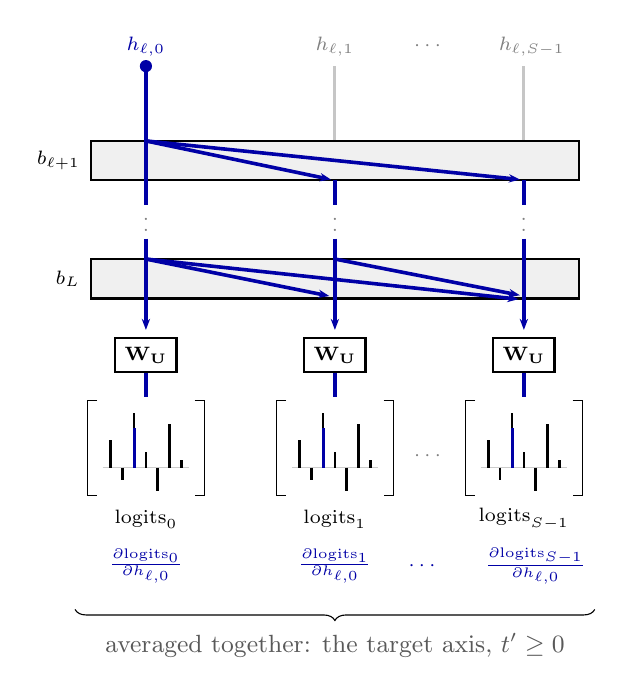
\begin{tikzpicture}[
  cord/.style={line width=1.1pt,gray!45},
  hcord/.style={line width=1.5pt,#1},
  harr/.style={line width=1.3pt,#1,-{Stealth[length=1.4mm]}},
]
\def\hc{blue!65!black}
% streams and stack (wide: full charts and one-row Jacobians below)
\foreach \X in {-2.4,0,2.4}{
  \draw[cord] (\X,0.35) -- (\X,-0.6);
  \draw[cord] (\X,-1.1) -- (\X,-1.42);
  \node[jlabS,gray] at (\X,-1.63) {$\vdots$};
  \draw[cord] (\X,-1.84) -- (\X,-2.1);}
\node[jlabS,gray] at (1.2,0.6) {$\cdots$};
\node[jlabS,\hc] at (-2.4,0.6) {$h_{\ell,0}$};
\node[jlabS,gray] at (0,0.6) {$h_{\ell,1}$};
\node[jlabS,gray] at (2.5,0.6) {$h_{\ell,S-1}$};
\node[draw,thick,fill=gray!12,minimum width=62mm,minimum height=5mm] (fA) at (0,-0.85) {};
\node[jlabS,left] at (fA.west) {$b_{\ell+1}$};
\node[draw,thick,fill=gray!12,minimum width=62mm,minimum height=5mm] (fB) at (0,-2.35) {};
\node[jlabS,left] at (fB.west) {$b_{L}$};
% the tapped latent floods every stream...
\fill[\hc] (-2.4,0.35) circle (2.2pt);
\draw[hcord=\hc] (-2.4,0.35) -- (-2.4,-1.42);
\draw[hcord=\hc] (-2.4,-1.84) -- (-2.4,-2.6);
\draw[harr=\hc] (-2.4,-0.6) -- (-0.05,-1.09);
\draw[harr=\hc] (-2.4,-0.6) -- (2.35,-1.09);
\draw[hcord=\hc] (0,-1.1) -- (0,-1.42);
\draw[hcord=\hc] (0,-1.84) -- (0,-2.6);
\draw[hcord=\hc] (2.4,-1.1) -- (2.4,-1.42);
\draw[hcord=\hc] (2.4,-1.84) -- (2.4,-2.6);
\draw[harr=\hc] (-2.4,-2.1) -- (-0.07,-2.57);
\draw[harr=\hc] (-2.4,-2.1) -- (2.33,-2.61);
\draw[harr=\hc] (0,-2.1) -- (2.35,-2.56);
% ...and every stream admits the (shared) unembedding
\foreach \X/\tl in {-2.4/{\logits_0},0/{\logits_1},2.4/{\logits_{S-1}}}{
  \draw[harr=\hc] (\X,-2.6) -- (\X,-3.0);
  \node[draw,thick,font=\scriptsize] at (\X,-3.32) {$\mathbf{W_U}$};
  \draw[hcord=\hc] (\X,-3.55) -- (\X,-3.85);
  \begin{scope}[shift={(\X,-4.75)}]\jlogits{0}{0}\end{scope}
  \draw[\hc,line width=1.1pt] (\X-0.15,-4.75) -- ++(0,0.5);
  \node[jlabS] at (\X,-5.4) {$\tl$};}
\node[jlabS,gray] at (1.2,-4.6) {$\cdots$};
% the row of Jacobians this fan produces
\node[jlabS,\hc] at (-2.4,-6.0) {$\frac{\partial \logits_0}{\partial h_{\ell,0}}$};
\node[jlabS,\hc] at (0,-6.0) {$\frac{\partial \logits_1}{\partial h_{\ell,0}}$};
\node[jlabS,\hc] at (1.13,-6.0) {$\cdots$};
\node[jlabS,\hc] at (2.55,-6.0) {$\frac{\partial \logits_{S-1}}{\partial h_{\ell,0}}$};
\draw[decorate,decoration={brace,mirror,amplitude=4pt}] (-3.3,-6.55) -- (3.3,-6.55)
      node[midway,below=5pt,jlab,gray!70!black]{averaged together: the target axis, $t' \ge 0$};
\end{tikzpicture}}
\caption{The complement to Figure~\ref{fig:context-strip}. Here, we highlight not the activations affecting a single logit vector, but a single activation and the many logit vectors it influences. One latent, $h_{\ell,0}$, and every logit vector it touches---its causal \textit{tails}.}
\label{fig:fan-out}
\end{figure}


Averaging over token position for a single context \(\textbf{C}_{\mathscr{p}}\)'s latents gives us the mean influence of layer \(\ell\) latents on future layer \(L\) latents.\footnote{It should be made clear that while there are 5050 distinct relationships being averaged together in the above example, we only need \(\dmodel\) iterations to compute this mean for the whole context \(\mathbf{C}_{\mathscr{p}}\). A forward pass seeded at layer \(\ell\) propagates to \textit{all} downstream positions in a single sweep, and the causal mask guarantees a source latent \(h_{\ell,t}\) reaches only targets \(t' \ge t\). So \(\dmodel\) forward or backward probes---one per model dimension---already carry every source's influence to every target it can touch, filling the whole-context Jacobian without ever visiting the 5050 pairs one at a time.}

\[J^{\mathscr{p}}_\ell = \mathbb{E}_{t \le t' < S_{\mathscr{p}}}\left[\frac{\partial h_{L,t'}}{\partial h_{\ell,t}}\right] = \mathbb{E}_{t \le t' < S_{\mathscr{p}}}\left[\frac{\partial R_\ell}{\partial h_{\ell}}\right]\]

Averaging \(|\mathscr{P}|\) of these context-specific Jacobians \(J^{\mathscr{p}}_\ell\) gives us \(J_\ell\).

\[J_\ell = \mathbb{E}_{\mathscr{p} \in \mathscr{P}}\left[J^{\mathscr{p}}_\ell\right]\]

As we saw in the definition above, with \(J_\ell\), we have \(\jlens_\ell\). Composition with \(\mathbf{W_U}\) is the static readout lens for layer \(L\) latents and \(J_\ell\) already approximates the translation from layer \(\ell\). We've tied the directions of layer \(\ell\) latents through layer \(L\) latents to tokens, at positions \(t' \ge t\). This gives \(\jlens\) bearing over future---not past, and not just \textit{immediate} future---verbalization. \footnote{Whether we fill this matrix by climbing backward or descending forward is the lesser question---the transport Jacobian \(J\) is square, so it costs \(\dmodel\) passes either way, and implementations generally climb, since backpropagation is the native idiom for it. The choice that earns its keep is \textit{how far to differentiate}. We could carry the derivative all the way through \(\mathbf{W_U}\) into logit space, filling \(\jlens\) a row at a time; but \(\mathbf{W_U}\) is a static matrix, and a static matrix \textit{is} its own Jacobian---re-deriving it on every pass buys nothing, and seeding in vocabulary space inflates the loop from \(\dmodel\) to \(|V|\). What these expected Jacobians really bring to the table is an approximation of the expected Jacobian of the network's \textit{nonlinear} processing, so that is the only stretch worth differentiating: from \(\ell\) to \(L\), \(\mathbb{R}^{\dmodel} \to \mathbb{R}^{\dmodel}\), probing the nonlinearity and nothing else. Compose the readout once at the end. Figure~\ref{fig:two-modes} draws both routes and why they land in the same place.} 




\subsection{Insightful Caveats}
What is the epistemological cost of averaging the local Jacobians into a global lens? An individually computed \(\frac{\partial h_{L,t'}}{\partial h_{\ell,t}} \in \mathbb{R}^{\dmodel \times \dmodel}\) is exact, but indexed to a specific point in layer \(\ell\)'s activation space. The earlier \(\ell\) is, the more of \(R_{\ell}\)'s higher-order curvature is being averaged away when we mean---first over positions into each context's \(J^{\mathscr{p}}_{\ell}\) and then over \(|\mathscr{P}|\) contexts---into the single \(J_{\ell}\). We average a layer's map over all (\(|\mathscr{P}| \times S\)) visited activations, pretending like local linear behavior is shared regionally when it really isn't. Figure~\ref{fig:tangents} attempts to stimulate intuitions about the information lost in local linear averaging of non-linear functions.

So then why average over contexts if we're creating an increasingly approximated object by doing so? The goal of \(\jlens\) is not to be an exact \(J\) of a specific \(\logits\) vector, with respect to a specific \(h\)---it is manifestly to be an aggregated, generalized map. While the complexity of the field of local functions defined in \(F\) (by way of \(R\))---the distinct attention paid to every unique context---is exactly what makes these models so powerful, the construction of \(\jlens\) is a \textit{postulation} that there is \textit{some} shared shape across the ways each context inspires speech in the model. Complex as \(F\) necessarily is, it is not some incompressibly arbitrary map. We lose information when we average local specificity into regional (dare we say) global approximations, but what we retain has general, nontrivial causal insight (as the \href{https://transformer-circuits.pub/2026/workspace/index.html}{paper} shows and we discuss in \S\ref{sec:jfindings}).\footnote{For what it is worth, \textit{training} adheres to the same postulation with respect to the effect of averaging over nonlinearity. It is hard to deny its success in postulating so. \(\jlens\) takes the same kinds of means and shows that---in the trained model, in \textit{activation} space---specificity is not the entire story.}

Averaging is a hypothesis. Here is how we test it: we can measure the magnitude of difference (\(\delta_{\ell,t,t'} = \left\|\frac{\partial h_{L,t'}}{\partial h_{\ell,t}} - J_\ell\right\|^2\)) between each local Jacobian and the global \(J_\ell\), and then average this to get an overall expected \textbf{dispersion} measure (\(\dispersion_\ell = \mathbb{E}_{t' \ge t,\, \mathscr{P}}[\delta_{\ell,t,t'}]\))\footnote{By the law of total variance the total splits as \(\dispersion_\ell = \dispersion^{\mathrm{w}}_\ell + \dispersion^{\mathrm{b}}_\ell\): a \textit{within-context} part \(\dispersion^{\mathrm{w}}_\ell = \mathbb{E}_{\mathscr{p}}\,\mathbb{E}_{t'\ge t}\bigl\lVert\frac{\partial h_{L,t'}}{\partial h_{\ell,t}} - J^{\mathscr{p}}_\ell\bigr\rVert^2\) (atoms scattering around their own prompt's mean---local curvature) plus a \textit{between-context} part \(\dispersion^{\mathrm{b}}_\ell = \mathbb{E}_{\mathscr{p}}\bigl\lVert J^{\mathscr{p}}_\ell - J_\ell\bigr\rVert^2\) (prompt-means disagreeing). We headline the total, but the between-part is the sharper object---it alone asks whether averaging \textit{over contexts} was warranted, i.e.\ how well the lens generalizes across them. The identity is exact provided both stages share one weighting over contexts: automatic for uniform \(S_{\mathscr{p}}\), and for mixed lengths one weights each context by its \((t,t')\) pair-count.} for a given \(J_\ell\).\footnote{Since the readout \(\mathbf{W_U}\) is a shared constant, it drops out of the difference, and only the nonlinear transport actually varies.} \(\dispersion_\ell\) is proportional to (1) the higher-order curvature of \(R_{\ell}\) and (2) variance in the sampled activations \(h_\ell\) in the \(h\)-region sampled. These factors compound, schematically: \(\dispersion_\ell \;\propto\; \left\|\frac{\partial^2 R_\ell}{\partial h_\ell^2}\right\|^2 \cdot \mathbb{E}\|h_\ell-\bar h_\ell\|^2\).


\(\dispersion\) fills in the detail productively smeared by \(J\) and \(\jlens\), complementing but not invalidating their causal importance.

%% The lens as the mean of tangents. Reference as Figure~\ref{fig:tangents}.
\begin{figure}[htbp]
\centering
\resizebox{0.8\textwidth}{!}{%
\begin{tikzpicture}[scale=1.35]
% axes
\draw[-{Stealth[length=1.8mm]}] (-0.2,0) -- (6.9,0);
\draw[-{Stealth[length=1.8mm]}] (0,-0.3) -- (0,2.6) node[jlabS,above] {$R_\ell(h)$ \scriptsize(one coord.\ of $h_L$)};
% the true nonlinear map
\draw[thick] plot[smooth] coordinates {(0.20,0.181) (0.41,0.365) (0.62,0.533) (0.83,0.681) (1.04,0.803) (1.25,0.895) (1.46,0.956) (1.67,0.984) (1.88,0.983) (2.09,0.955) (2.30,0.906) (2.51,0.842) (2.72,0.769) (2.93,0.696) (3.14,0.630) (3.35,0.579) (3.56,0.549) (3.77,0.544) (3.98,0.569) (4.19,0.626) (4.40,0.715) (4.61,0.834) (4.82,0.979) (5.03,1.145) (5.24,1.327) (5.45,1.517) (5.66,1.708) (5.87,1.891) (6.08,2.060) (6.29,2.209) (6.50,2.331)};
\node[jlabS,right] at (6.45,2.32) {$R_\ell$};
% per-context tangents at the visited activations
\draw[gray!55,thin] (1.00,0.956) -- (2.40,1.016);
\draw[gray!55,thin] (1.30,1.069) -- (2.70,0.871);
\draw[gray!55,thin] (1.55,1.100) -- (2.95,0.739);
\draw[gray!55,thin] (1.80,1.076) -- (3.20,0.614);
\draw[gray!55,thin] (2.05,1.005) -- (3.45,0.512);
\draw[gray!55,thin] (2.30,0.899) -- (3.70,0.447);
\draw[gray!55,thin] (2.65,0.719) -- (4.05,0.440);
\draw[gray!55,thin] (3.20,0.460) -- (4.60,0.652);
\fill (1.70,0.986) circle (1.3pt);
\fill (2.00,0.970) circle (1.3pt);
\fill (2.25,0.919) circle (1.3pt);
\fill (2.50,0.845) circle (1.3pt);
\fill (2.75,0.759) circle (1.3pt);
\fill (3.00,0.673) circle (1.3pt);
\fill (3.35,0.579) circle (1.3pt);
\fill (3.90,0.556) circle (1.3pt);
% the mean of the tangents: the lens
\draw[jvio,line width=1.3pt] (0.5,1.171) -- (6.1,0.174);
\node[jlabS,jvio,right] at (6.15,0.36) {$J_\ell$: the mean tangent};
% where the line lies
\draw[gray!60,dashed] (5.4,0.299) -- (5.4,1.472);
\fill[gray!60] (5.4,1.472) circle (1.1pt);
\node[jlabS,gray!70!black,align=center,right] at (5.52,1.0) {far from the data,\\the line lies};
% dispersion note
\node[jlabS,gray!70!black,align=center] at (1.35,2.15) {curvature makes the\\tangents disagree:\\\emph{dispersion}};
\draw[gray!60,thin,-{Stealth[length=1.3mm]}] (1.75,1.85) to[out=-60,in=140] (2.42,1.05);
% ==== dispersion strip: shared h-axis, F and mean removed, delta bars added ====
% faint droplines: each dot above sits directly over its delta bar below (shared h)
\foreach \x/\bt in {1.70/-1.561,2.00/-1.988,2.25/-1.943,2.50/-1.792,2.75/-1.727,3.00/-1.811,3.35/-1.996,3.90/-1.106}{
  \draw[gray!30,thin,dotted] (\x,-0.12) -- (\x,\bt);}
% the bars: delta_i = || J_ell(h_i) - J_ell ||^2, at the same x as each dot above
\foreach \x/\h in {1.70/0.439,2.00/0.012,2.25/0.057,2.50/0.208,2.75/0.273,3.00/0.189,3.35/0.004,3.90/0.894}{
  \fill[jvio!72] (\x-0.055,-2.0) rectangle (\x+0.055,{-2.0+\h});}
% net dispersion = mean bar height, full width
\draw[jvio,dashed,line width=1pt] (0,-1.741) -- (6.9,-1.741);
\node[jlabS,jvio,above] at (5.5,-1.735) {$\dispersion_\ell=\mathbb{E}[\delta]\approx0.029$};
\node[jlabS,gray!70!black,align=center] at (5.15,-1.12) {this context's $\delta$\\ dominates};
\draw[gray!55,thin,-{Stealth[length=1.2mm]}] (4.45,-1.16) to[out=180,in=55] (3.99,-1.18);
% delta-axis (black) at x=0, colinear with the top y-axis
\draw[-{Stealth[length=1.8mm]}] (0,-2.06) -- (0,-0.88) node[jlabS,above left=0pt] {$\delta(h)$};
\node[jlabS,left] at (-0.06,-2.0) {$0$};
% the shared x-axis (black), labeled here beneath the lower panel
\draw[-{Stealth[length=1.8mm]}] (-0.2,-2.0) -- (6.9,-2.0) node[jlabS,below left=1pt] {$h$ \scriptsize(one direction of $\mathbb{R}^{\dmodel}$)};
% region annotation, now beneath the shared axis
\draw[decorate,decoration={brace,mirror,amplitude=3pt}] (1.55,-2.18) -- (4.05,-2.18)
      node[midway,below=3pt,jlabS,gray!70!black] {region visited by real activations};
\end{tikzpicture}}
\caption{What the lens is: the average of the local linear behaviors $J_\ell(h) = \frac{\partial h_L}{\partial h}$---i.e.\ the atom $\frac{\partial h_{L,t'}}{\partial h_{\ell,t}}$ at each visited latent $h = h_{\ell,t}$---across the activations the model actually visits (dots; one gray tangent each). Where $R_\ell$ curves within the visited region, the tangents fan---that spread \emph{is} the dispersion $\dispersion_\ell = \mathbb{E}\|J_\ell(h)-J_\ell\|^2$. And the mean tangent is a local instrument: far from the sampled region, the line and the function part ways. The lower panel makes the spread concrete: each bar is one visited latent's $\delta = \|J_\ell(h)-J_\ell\|^2$---how far its tangent tilts from the mean---and $\dispersion_\ell$ is simply their average, pulled up here by the lone high-curvature latent at the region's right edge.}
\label{fig:tangents}
\end{figure}



\section{J-space}\label{sec:jspace}

Where \(\jlens\) shines in the \textit{synthesis} it makes of causal relationships into a single object, it blinds with its potent density. The \textbf{J-space} is a kind of prism we fit to the information that pours into \(\jlens\), reducing it to a sparse few of its directions and focusing its information into distinct beams of practical insight. \(\jlens\) colors the \(\dmodel\)-sized latent states of the model with what it means for all \(|V|\) concepts in its available grasp, but do we feel intuitively that every thought in our heads should be put in relation to \textit{every} word we can possibly utter? Any \(h\) must be reducible to only those directions in token space that really count, right? Beyond the reduction the \textbf{J-space} provides for the purposes of interpreting internal state, if we want to affect change in the model's behavior, we'd hope that we wouldn't have to tweak \textit{every single} source, but only a privileged few, right? 

Knowing the normalized alignment vector \(\jlens(h)\) of any latent is valuable, but \(\jlens\) itself (and the vocabulary it speaks to!) is highly redundant. If \(h\) scores highly with a token, ``\texttt{dog}'', then it will likely align with tokens such as ``\texttt{dogs}'', ``\texttt{canine}'', and ``\texttt{puppy}''.\footnote{These words specifically may not be tokens in real LLMs, but it is an idealized example.} Knowing one of these practically tells us the other. Taking the top 10 scoring tokens from \(\jlens(h)\) might only give us 2 or 3 truly distinct concepts.

The \textbf{J-space} \(\jspace\) is defined to bring information-retaining \textbf{sparsity} to the redundancy of \(\jlens\)-space. \(\jspace\) is an \textit{intensionally} as opposed to \textit{extensionally} defined space, never fully enumerated as an object like \(\jlens\) but instead specified by a constrained recipe for finding its members.\footnote{For one thing, it is an \textit{uncountably} infinite space---a union of finitely many cones, but each cone a continuum of points---so we could never compact it into an object like \(\jlens\).} The \textbf{J-space} \textit{decomposition} \(\jspace(h)\) of an activation \(h\) is the closest point \textit{in the \textbf{J-space}} to \(h\) itself. Once \(\jlens\)-space is made sparse, the meaningful conceptual decomposition of the residual stream is fast-tracked and principled, allowing for efficiently pointed interventions.

\subsection{Computation}\label{sec:jspacecomp}

The \textbf{J-space} \(\jspace_\ell\) in layer \(\ell\) is defined as the set of all points reachable by a sparse, nonnegative decomposition of up to \(k\) rows of \(\jlens\), where \(k\) is our sparsity constraint. Anthropic denotes it as a \textit{union of cones} in \(\mathbb{R}^{\dmodel}\), where each cone is made up of a set of \(k\) directions (rows drawn from \(\jlens\)), each with a nonnegative coefficient. Writing \(\mathscr{m}_{v}\) for the row of \(\jlens\) belonging to token \(v\), and collecting the coefficients into a single sparse, nonnegative vector \(c \in \mathbb{R}^{|V|}_{\ge 0}\) with at most \(k\) nonzero entries (\(\|c\|_0 \le k\)), the space is
\[ \jspace \;=\; \bigl\{\, \jlens^{\!\top} c \;:\; c \ge 0,\ \|c\|_0 \le k \,\bigr\}, \qquad \jlens^{\!\top} c \;=\; \sum_{v=1}^{|V|} c_v\, \mathscr{m}_{v} \]

The \textbf{J-space} \textit{decomposition} \(\jspace(h)\) of a latent \(h\) is then defined as the point in \(\jspace\) that is closest to \(h\).

\[ \jspace(h) \;=\; \jlens^{\!\top} c^\star, \qquad c^\star \;=\; \argmin_{\substack{c \,\in\, \mathbb{R}^{|V|}_{\ge 0} \\ \|c\|_0 \,\le\, k}} \bigl\| \jlens^{\!\top} c - h \bigr\|_2^2  \]

\(c^\star\) is our prism on the overcomplete white light that is \(\jlens\). Once fit, \(c^\star\) sifts the \(k\) directions in \(\jlens\)-space (\(\in \mathbb{R}^{\dmodel}\)) that best reconstruct \(h\). If each row of \(\jlens\) denotes a direction of steepest logit-increase for each token, then \(\jspace(h)\) puts together a non-redundant report of the \(k\) directions in token space that best describe the model's disposition.

While the notation defining \(\jspace(h)\) is succinct, choosing the best \(k\) rows out of a \(|V|\)-term dictionary is NP-hard, so we solve it greedily. One objective---\textit{reconstruct \(h\) as closely as possible with only \(k\) rows}---forces two oscillating, complementary operations: \textit{select} directions against the residual \(r\) (which progressively shrinks during the optimization), but always \textit{fit} against \(h\). Every \textit{next} direction \(\mathscr{m}\) is the one most aligned with \textit{what still needs to be covered} (the residual, \(r\)). After each next direction selection, we see how well the working set of directions reconstructs the ultimate objective, \textit{h}. \textit{Diversity} among the \(k\) rows of \(\jlens\) that we select is never an imposed rule---it falls out of greedily \textit{selecting} against the residual but \textit{fitting} against the target. The selected rows are not thereby \textit{mutually orthogonal} (with an overcomplete, correlated dictionary they generally are not); what emerges is only that we never waste one of our \(k\) slots re-selecting a direction the working set already covers, since after each refit the residual is (near-)orthogonal to everything we have already captured. Algorithm~\ref{alg:jspace} displays the \textit{outer} algorithm for selecting directions, while Algorithm~\ref{alg:fit} (\textsc{Fit}) specifies how those directions are fit. Because \textsc{Fit} re-solves \textit{all} of the active coefficients against \(h\) at every round---rather than freezing past coefficients and only appending the new one---the procedure is, strictly, nonnegative \textit{orthogonal} matching pursuit, not the original matching pursuit.\footnote{Orthogonal matching pursuit: Y.~C. Pati, R.~Rezaiifar, and P.~S. Krishnaprasad, \textit{Orthogonal Matching Pursuit: Recursive Function Approximation with Applications to Wavelet Decomposition}, Proc.\ 27th Asilomar Conf.\ on Signals, Systems and Computers, \href{https://doi.org/10.1109/ACSSC.1993.342465}{1993}.}

% ===== J-space decomposition algorithm (matching pursuit + refit) =====
% Reference it in prose as: Algorithm~\ref{alg:jspace}  (renders "Algorithm 1", clickable via hyperref).
% This is a working draft --- fill in / adjust the steps, comments, and any stopping rule as you like.
\begin{algorithm}[htbp]
\caption{\(\jspace(h)\)}
\label{alg:jspace}
\begin{algorithmic}[1]
\Require latent \(h \in \mathbb{R}^{\dmodel}\);\ \ J-lens rows \(\mathscr{m}_{v}\) for \(v = 0,\dots,|V|-1\);\ \ sparsity budget \(k\)
\Ensure sparse nonnegative \(c \in \mathbb{R}^{|V|}_{\ge 0}\) with \(\|c\|_0 \le k\);\ \ decomposition \(\jspace(h) = \jlens^{\!\top} c\)
\State \(r \gets h\);\quad \(A \gets \varnothing\);\quad \(c \gets \mathbf{0}\) \Comment{residual, active support, coefficients}
\For{\(j = 1\) \textbf{to} \(k\)} \Comment{outer loop: grow the support}
  \State \(\displaystyle v^\star \gets \argmax_{v}\ \frac{\langle \mathscr{m}_{v},\, r\rangle}{\lVert \mathscr{m}_{v}\rVert}\) \Comment{select against the residual \(r\) --- the fastest error drop}
  \State \(A \gets A \cup \{v^\star\}\) \Comment{selecting against \(r\), not \(h\), keeps the support diverse}
  \State \(c_A \gets\) \textsc{Fit}\((A, h)\) \Comment{fit the weights against \(h\) itself (Alg.~\ref{alg:fit})}
  \State \(\displaystyle r \gets h - \sum_{v \in A} (c_A)_v\, \mathscr{m}_{v}\) \Comment{what \(\jspace\) still cannot explain}
\EndFor
\State \Return \(c\) (zero off \(A\)),\ \ \(\jspace(h) = \jlens^{\!\top} c\)
\end{algorithmic}
\end{algorithm}

% ===== The inner fit, called from Algorithm 1 line 5. Reference as Algorithm~\ref{alg:fit}. =====
% Convergence story: projected gradient descent, run until the residual stops shrinking.
% NOTE: the gradient g_v = -<m_v, r> is the SAME alignment-with-residual used to SELECT in Alg 1 ---
% selection picks the single most-aligned row; the fit nudges every active row by its alignment.
\begin{algorithm}[htbp]
\caption{\textsc{Fit}\((A, h)\)}
\label{alg:fit}
\begin{algorithmic}[1]
\Require active support \(A\); latent \(h\); J-lens rows \(\mathscr{m}_{v}\); step size \(\eta\)
\Ensure \(c_A \ge 0\) minimizing \(\bigl\lVert \sum_{v \in A}(c_A)_v\,\mathscr{m}_{v} - h \bigr\rVert_2^2\)
\State \(c_A \gets \mathbf{0}\)
\Repeat
  \State \(\displaystyle r \gets h - \sum_{v \in A}(c_A)_v\,\mathscr{m}_{v}\) \Comment{residual under the current weights}
  \State \(g_v \gets -\langle \mathscr{m}_{v},\, r\rangle \quad \forall\, v \in A\) \Comment{gradient: (minus) each row's alignment with \(r\)}
  \State \(c_A \gets \max\!\bigl(\mathbf{0},\; c_A - \eta\, g\bigr)\) \Comment{descend, then project back onto \(c_A \ge 0\)}
\Until{\(\lVert r\rVert\) stops shrinking}
\State \Return \(c_A\)
\end{algorithmic}
\end{algorithm}


Algorithm~\ref{alg:fit} should seem familiar: it is gradient descent! Write the error as \(e \equiv \hat{s} - h = \sum_w c_w\, \mathscr{m}_w - h = -r\), where \(\hat{s}\) is the running reconstruction of \(h\) under the current coefficients, so the loss is
\[ L(c) \;=\; \bigl\lVert \hat{s} - h\bigr\rVert_2^2 \;=\; \lVert e\rVert^2 \;=\; e \cdot e \]
Differentiating with respect to a single coefficient \(c_v\),
\[ \frac{\partial L}{\partial c_v} \;=\; \frac{\partial}{\partial c_v}\,\bigl(e \cdot e\bigr) \;=\; 2\, e \cdot \frac{\partial e}{\partial c_v}, \]
the inner derivative picks out a single term,
\[ \frac{\partial e}{\partial c_v} \;=\; \frac{\partial}{\partial c_v}\Bigl(\sum_w c_w\, \mathscr{m}_w - h\Bigr) \;=\; \mathscr{m}_v \]
since \(h\) and every \(c_w\) with \(w \neq v\) are constant in \(c_v\). Substituting back,
\[ \frac{\partial L}{\partial c_v} \;=\; 2\, e \cdot \mathscr{m}_v \;=\; 2(\hat{s}-h)\cdot \mathscr{m}_v \;=\; 2(-r)\cdot \mathscr{m}_v \;=\; -2\,\langle \mathscr{m}_v,\, r\rangle \]

At every turn of the optimization, \(r\) is the vector representing all of \(h\) that we have not reconstructed. It is a \textit{direction} in which we want to move, not a point at which we want to arrive. The more we nudge \(\sum_{v \in A}(c_A)_v\,\mathscr{m}_{v}\) towards \(r\), the more \(r\) disappears.\footnote{Because \(r = h - \sum_{v \in A}(c_A)_v\,\mathscr{m}_{v}\)!} We want to adjust each coefficient \(c_v\) so it supports this directional goal and brings its corresponding \(\mathscr{m}_v\) to where it needs to be to cancel more of \(r\). What is the relationship between \(c_v\) and \(r\)? It is exactly (proportional to) \(\langle \mathscr{m}_v,\, r\rangle\)!

The motivation for the \textbf{J-space} decomposition \(\jspace(h)\) of a latent \(h\) is plain: positively include the \(k\) distinct token-influence directions of \(h\)-space that can reconstruct \(h\) the best. ``Describe the model's disposition in \(k\) words, each with a weight." The \textit{algorithm} for computing it, though, is even more plain and elegant. At every turn of the outer algorithm, select the direction that best eats up the work we have left to do (\(r\)).\footnote{This is what buys us the diversity noted above. In an idealized view, whatever directions are grabbed in one round against \(r\) are `claimed' from then on, removed from \(r'\), and `unwanted' by the subsequent dot products against \(r'\).} Then for each working set of directions, figure out the best way to combine them to reconstruct the information we actually want to reconstruct, \(h\). The algorithm is so nice because its goal is so interpretable and intuitive and its methods are so familiar to anyone who has worked with neural networks. Interestingly, it was originally introduced (under the name of \textit{matching pursuit}) in the context of continuous signal processing by Mallat and Zhang \href{https://doi.org/10.1109/78.258082}{(1993)}.\footnote{S.~G. Mallat and Z.~Zhang, \textit{Matching Pursuits with Time-Frequency Dictionaries}, IEEE Trans.\ Signal Processing, 41(12):3397--3415, 1993.} Continuous sinusoidal waves that are composed of pure frequencies, each at a specific amplitude (and phase), resemble vectors that are composed of different directions. The motivation to deconstruct them is the same: \textit{which frequencies are present in this signal?} Better yet, \textit{what are the \textbf{top k }frequencies that could approximate this signal?} Each pure frequency brings something distinct to the table, like each direction of a vector space. (1) How do you find the single pure frequency that best aligns with a sinusoid (be it a raw signal or a residual)? Dot product! This gives us the Discrete Fourier Transform. (2) If you have a fixed set of pure frequencies, how do you figure out their best combination to reconstruct a sinusoid? Gradient descent!  Figure~\ref{fig:jspace-freq} celebrates this alignment in methods and motivations, honoring the original instantiation of the matching pursuit algorithm which we use to compute \(\jspace(h)\), and stimulating your intuition for what reconstruction really looks like. 

\begin{figure}[htbp]
\centering
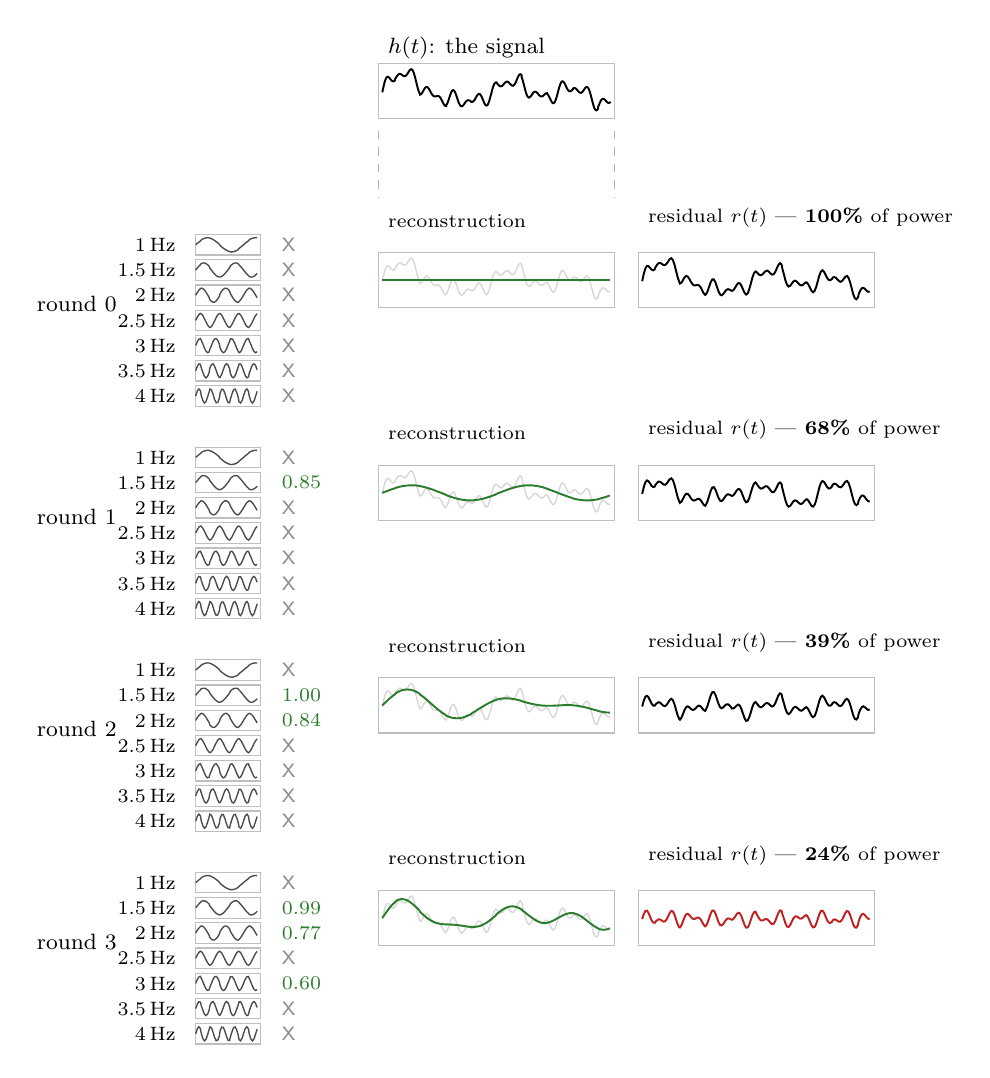
\begin{tikzpicture}[x=1cm,y=1cm,lab/.style={font=\footnotesize},lil/.style={font=\scriptsize},wv/.style={line width=.7pt},bx/.style={draw=black!25,line width=.4pt}]
% GENERATED by scripts/gen_freq_figure.py --- do not hand-edit; re-run the script.
% Coefficients and residual percentages come from a real nonnegative-OMP run.
\def\hghost{%
(2.95,-0.813) (2.97,-0.721) (2.99,-0.652) (3.01,-0.618) (3.03,-0.620) (3.05,-0.642) (3.07,-0.666) (3.09,-0.674) (3.11,-0.661) (3.12,-0.633)
(3.14,-0.602) (3.16,-0.582) (3.18,-0.580) (3.20,-0.592) (3.22,-0.606) (3.24,-0.608) (3.26,-0.591) (3.28,-0.561) (3.30,-0.531) (3.32,-0.520)
(3.34,-0.543) (3.36,-0.600) (3.38,-0.680) (3.40,-0.760) (3.42,-0.819) (3.43,-0.842) (3.45,-0.829) (3.47,-0.795) (3.49,-0.761) (3.51,-0.745)
(3.53,-0.754) (3.55,-0.784) (3.57,-0.821) (3.59,-0.851) (3.61,-0.865) (3.63,-0.864) (3.65,-0.859) (3.67,-0.864) (3.69,-0.886) (3.71,-0.923)
(3.73,-0.963) (3.75,-0.986) (3.76,-0.980) (3.78,-0.943) (3.80,-0.884) (3.82,-0.826) (3.84,-0.790) (3.86,-0.790) (3.88,-0.826) (3.90,-0.884)
(3.92,-0.943) (3.94,-0.981) (3.96,-0.991) (3.98,-0.975) (4.00,-0.946) (4.02,-0.922) (4.04,-0.913) (4.06,-0.919) (4.08,-0.931) (4.09,-0.936)
(4.11,-0.923) (4.13,-0.895) (4.15,-0.860) (4.17,-0.837) (4.19,-0.838) (4.21,-0.867) (4.23,-0.914) (4.25,-0.959) (4.27,-0.982) (4.29,-0.968)
(4.31,-0.916) (4.33,-0.842) (4.35,-0.766) (4.37,-0.711) (4.39,-0.688) (4.40,-0.693) (4.42,-0.714) (4.44,-0.733) (4.46,-0.736) (4.48,-0.723)
(4.50,-0.700) (4.52,-0.682) (4.54,-0.678) (4.56,-0.692) (4.58,-0.714) (4.60,-0.729) (4.62,-0.724) (4.64,-0.695) (4.66,-0.649) (4.68,-0.605)
(4.70,-0.583) (4.72,-0.598) (4.73,-0.650) (4.75,-0.726) (4.77,-0.802) (4.79,-0.858) (4.81,-0.880) (4.83,-0.870) (4.85,-0.843) (4.87,-0.816)
(4.89,-0.805) (4.91,-0.814) (4.93,-0.836) (4.95,-0.857) (4.97,-0.866) (4.99,-0.859) (5.01,-0.841) (5.03,-0.826) (5.04,-0.828) (5.06,-0.853)
(5.08,-0.893) (5.10,-0.933) (5.12,-0.952) (5.14,-0.936) (5.16,-0.886) (5.18,-0.813) (5.20,-0.739) (5.22,-0.689) (5.24,-0.673) (5.26,-0.692)
(5.28,-0.732) (5.30,-0.772) (5.32,-0.797) (5.34,-0.799) (5.36,-0.784) (5.37,-0.766) (5.39,-0.759) (5.41,-0.768) (5.43,-0.789) (5.45,-0.811)
(5.47,-0.820) (5.49,-0.809) (5.51,-0.782) (5.53,-0.755) (5.55,-0.745) (5.57,-0.767) (5.59,-0.823) (5.61,-0.899) (5.63,-0.975) (5.65,-1.027)
(5.67,-1.042) (5.69,-1.020) (5.70,-0.976) (5.72,-0.930) (5.74,-0.901) (5.76,-0.896) (5.78,-0.911) (5.80,-0.933) (5.82,-0.947) (5.84,-0.943)}
\node[lab,anchor=west] at (2.9,1.45){$h(t)$: the signal};
\draw[bx] (2.9,0.55) rectangle (5.9,1.25);
\draw[wv,black] plot coordinates {
(2.95,0.887) (2.96,0.935) (2.97,0.979) (2.98,1.018) (2.99,1.048) (3.00,1.070) (3.01,1.082) (3.02,1.085) (3.03,1.080) (3.04,1.070)
(3.05,1.058) (3.06,1.045) (3.07,1.034) (3.08,1.027) (3.09,1.026) (3.10,1.029) (3.11,1.039) (3.11,1.052) (3.12,1.067) (3.13,1.084)
(3.14,1.098) (3.15,1.110) (3.16,1.118) (3.17,1.121) (3.18,1.120) (3.19,1.115) (3.20,1.108) (3.21,1.100) (3.22,1.094) (3.23,1.091)
(3.24,1.092) (3.25,1.098) (3.26,1.109) (3.27,1.123) (3.28,1.139) (3.29,1.156) (3.30,1.169) (3.31,1.178) (3.32,1.180) (3.33,1.173)
(3.34,1.157) (3.35,1.133) (3.36,1.100) (3.37,1.062) (3.38,1.020) (3.39,0.978) (3.40,0.940) (3.41,0.907) (3.42,0.881) (3.43,0.865)
(3.43,0.858) (3.44,0.861) (3.45,0.871) (3.46,0.886) (3.47,0.905) (3.48,0.923) (3.49,0.939) (3.50,0.950) (3.51,0.955) (3.52,0.954)
(3.53,0.946) (3.54,0.933) (3.55,0.916) (3.56,0.897) (3.57,0.879) (3.58,0.862) (3.59,0.849) (3.60,0.840) (3.61,0.835) (3.62,0.834)
(3.63,0.836) (3.64,0.839) (3.65,0.841) (3.66,0.840) (3.67,0.836) (3.68,0.827) (3.69,0.814) (3.70,0.796) (3.71,0.777) (3.72,0.756)
(3.73,0.737) (3.74,0.723) (3.75,0.714) (3.76,0.713) (3.76,0.720) (3.77,0.735) (3.78,0.757) (3.79,0.785) (3.80,0.816) (3.81,0.846)
(3.82,0.874) (3.83,0.896) (3.84,0.910) (3.85,0.915) (3.86,0.910) (3.87,0.896) (3.88,0.874) (3.89,0.846) (3.90,0.816) (3.91,0.785)
(3.92,0.757) (3.93,0.735) (3.94,0.719) (3.95,0.710) (3.96,0.709) (3.97,0.715) (3.98,0.725) (3.99,0.739) (4.00,0.754) (4.01,0.767)
(4.02,0.778) (4.03,0.784) (4.04,0.787) (4.05,0.785) (4.06,0.781) (4.07,0.775) (4.08,0.769) (4.08,0.765) (4.09,0.764) (4.10,0.768)
(4.11,0.777) (4.12,0.789) (4.13,0.805) (4.14,0.823) (4.15,0.840) (4.16,0.854) (4.17,0.863) (4.18,0.866) (4.19,0.862) (4.20,0.851)
(4.21,0.833) (4.22,0.811) (4.23,0.786) (4.24,0.762) (4.25,0.741) (4.26,0.725) (4.27,0.718) (4.28,0.720) (4.29,0.732) (4.30,0.754)
(4.31,0.784) (4.32,0.819) (4.33,0.858) (4.34,0.897) (4.35,0.934) (4.36,0.965) (4.37,0.989) (4.38,1.005) (4.39,1.012) (4.40,1.013)
(4.40,1.007) (4.41,0.997) (4.42,0.986) (4.43,0.975) (4.44,0.967) (4.45,0.963) (4.46,0.964) (4.47,0.968) (4.48,0.977) (4.49,0.988)
(4.50,1.000) (4.51,1.010) (4.52,1.018) (4.53,1.022) (4.54,1.022) (4.55,1.017) (4.56,1.008) (4.57,0.997) (4.58,0.986) (4.59,0.977)
(4.60,0.971) (4.61,0.970) (4.62,0.976) (4.63,0.987) (4.64,1.005) (4.65,1.027) (4.66,1.051) (4.67,1.075) (4.68,1.095) (4.69,1.110)
(4.70,1.117) (4.71,1.114) (4.72,1.102) (4.72,1.080) (4.73,1.050) (4.74,1.014) (4.75,0.974) (4.76,0.935) (4.77,0.898) (4.78,0.866)
(4.79,0.842) (4.80,0.827) (4.81,0.820) (4.82,0.822) (4.83,0.830) (4.84,0.843) (4.85,0.857) (4.86,0.872) (4.87,0.884) (4.88,0.892)
(4.89,0.895) (4.90,0.893) (4.91,0.886) (4.92,0.876) (4.93,0.864) (4.94,0.853) (4.95,0.843) (4.96,0.836) (4.97,0.834) (4.98,0.835)
(4.99,0.841) (5.00,0.850) (5.01,0.859) (5.02,0.868) (5.03,0.874) (5.04,0.876) (5.04,0.872) (5.05,0.862) (5.06,0.847) (5.07,0.828)
(5.08,0.807) (5.09,0.786) (5.10,0.767) (5.11,0.754) (5.12,0.748) (5.13,0.751) (5.14,0.764) (5.15,0.785) (5.16,0.814) (5.17,0.849)
(5.18,0.887) (5.19,0.926) (5.20,0.961) (5.21,0.990) (5.22,1.011) (5.23,1.024) (5.24,1.027) (5.25,1.021) (5.26,1.008) (5.27,0.989)
(5.28,0.968) (5.29,0.947) (5.30,0.928) (5.31,0.913) (5.32,0.903) (5.33,0.899) (5.34,0.901) (5.35,0.907) (5.36,0.916) (5.37,0.925)
(5.37,0.934) (5.38,0.939) (5.39,0.941) (5.40,0.939) (5.41,0.932) (5.42,0.922) (5.43,0.911) (5.44,0.899) (5.45,0.889) (5.46,0.882)
(5.47,0.880) (5.48,0.883) (5.49,0.891) (5.50,0.903) (5.51,0.918) (5.52,0.932) (5.53,0.945) (5.54,0.953) (5.55,0.955) (5.56,0.948)
(5.57,0.933) (5.58,0.909) (5.59,0.877) (5.60,0.840) (5.61,0.801) (5.62,0.761) (5.63,0.725) (5.64,0.695) (5.65,0.673) (5.66,0.661)
(5.67,0.658) (5.68,0.665) (5.69,0.680) (5.69,0.700) (5.70,0.724) (5.71,0.748) (5.72,0.770) (5.73,0.788) (5.74,0.799) (5.75,0.805)
(5.76,0.804) (5.77,0.798) (5.78,0.789) (5.79,0.778) (5.80,0.767) (5.81,0.758) (5.82,0.753) (5.83,0.753) (5.84,0.757) (5.85,0.765)
};
\draw[black!30,dashed,line width=.4pt] (2.9,0.4)--(2.9,-0.45); \draw[black!30,dashed,line width=.4pt] (5.9,0.4)--(5.9,-0.45);
\begin{scope}[shift={(0,-0.7)}]
\node[lab,anchor=east] at (-0.3,-1.1){round 0};
\node[lil,anchor=east] at (0.45,-0.35){1\,Hz};
\draw[bx] (0.58,-0.48) rectangle (1.4,-0.22);
\draw[black!70,line width=.5pt] plot coordinates {
(0.58,-0.350) (0.60,-0.333) (0.62,-0.316) (0.64,-0.301) (0.65,-0.288) (0.67,-0.276) (0.69,-0.268) (0.71,-0.262) (0.73,-0.260) (0.75,-0.261) (0.76,-0.265) (0.78,-0.272)
(0.80,-0.283) (0.82,-0.295) (0.84,-0.310) (0.86,-0.326) (0.88,-0.343) (0.89,-0.360) (0.91,-0.377) (0.93,-0.392) (0.95,-0.407) (0.97,-0.419) (0.99,-0.429) (1.01,-0.436)
(1.02,-0.439) (1.04,-0.440) (1.06,-0.437) (1.08,-0.431) (1.10,-0.422) (1.12,-0.411) (1.13,-0.397) (1.15,-0.381) (1.17,-0.365) (1.19,-0.348) (1.21,-0.330) (1.23,-0.314)
(1.25,-0.299) (1.26,-0.286) (1.28,-0.275) (1.30,-0.267) (1.32,-0.262) (1.34,-0.260) (1.36,-0.261)
};
\node[lil,black!45,anchor=west] at (1.55,-0.35){\textsf{X}};
\node[lil,anchor=east] at (0.45,-0.67){1.5\,Hz};
\draw[bx] (0.58,-0.80) rectangle (1.4,-0.54);
\draw[black!70,line width=.5pt] plot coordinates {
(0.58,-0.670) (0.60,-0.645) (0.62,-0.621) (0.64,-0.602) (0.65,-0.588) (0.67,-0.581) (0.69,-0.581) (0.71,-0.588) (0.73,-0.603) (0.75,-0.622) (0.76,-0.646) (0.78,-0.671)
(0.80,-0.697) (0.82,-0.720) (0.84,-0.739) (0.86,-0.753) (0.88,-0.759) (0.89,-0.759) (0.91,-0.751) (0.93,-0.737) (0.95,-0.717) (0.97,-0.693) (0.99,-0.668) (1.01,-0.642)
(1.02,-0.619) (1.04,-0.600) (1.06,-0.587) (1.08,-0.581) (1.10,-0.581) (1.12,-0.590) (1.13,-0.604) (1.15,-0.624) (1.17,-0.648) (1.19,-0.674) (1.21,-0.699) (1.23,-0.722)
(1.25,-0.741) (1.26,-0.753) (1.28,-0.760) (1.30,-0.758) (1.32,-0.750) (1.34,-0.735) (1.36,-0.715)
};
\node[lil,black!45,anchor=west] at (1.55,-0.67){\textsf{X}};
\node[lil,anchor=east] at (0.45,-0.99){2\,Hz};
\draw[bx] (0.58,-1.12) rectangle (1.4,-0.86);
\draw[black!70,line width=.5pt] plot coordinates {
(0.58,-0.990) (0.60,-0.956) (0.62,-0.928) (0.64,-0.908) (0.65,-0.900) (0.67,-0.905) (0.69,-0.923) (0.71,-0.950) (0.73,-0.983) (0.75,-1.017) (0.76,-1.047) (0.78,-1.069)
(0.80,-1.079) (0.82,-1.077) (0.84,-1.062) (0.86,-1.037) (0.88,-1.005) (0.89,-0.970) (0.91,-0.939) (0.93,-0.915) (0.95,-0.902) (0.97,-0.901) (0.99,-0.914) (1.01,-0.937)
(1.02,-0.968) (1.04,-1.002) (1.06,-1.035) (1.08,-1.061) (1.10,-1.076) (1.12,-1.080) (1.13,-1.070) (1.15,-1.049) (1.17,-1.019) (1.19,-0.985) (1.21,-0.952) (1.23,-0.924)
(1.25,-0.906) (1.26,-0.900) (1.28,-0.907) (1.30,-0.926) (1.32,-0.954) (1.34,-0.988) (1.36,-1.021)
};
\node[lil,black!45,anchor=west] at (1.55,-0.99){\textsf{X}};
\node[lil,anchor=east] at (0.45,-1.31){2.5\,Hz};
\draw[bx] (0.58,-1.44) rectangle (1.4,-1.18);
\draw[black!70,line width=.5pt] plot coordinates {
(0.58,-1.310) (0.60,-1.269) (0.62,-1.236) (0.64,-1.221) (0.65,-1.225) (0.67,-1.249) (0.69,-1.286) (0.71,-1.328) (0.73,-1.367) (0.75,-1.393) (0.76,-1.400) (0.78,-1.387)
(0.80,-1.357) (0.82,-1.316) (0.84,-1.274) (0.86,-1.240) (0.88,-1.222) (0.89,-1.223) (0.91,-1.244) (0.93,-1.280) (0.95,-1.322) (0.97,-1.362) (0.99,-1.390) (1.01,-1.400)
(1.02,-1.390) (1.04,-1.362) (1.06,-1.322) (1.08,-1.280) (1.10,-1.244) (1.12,-1.223) (1.13,-1.222) (1.15,-1.240) (1.17,-1.274) (1.19,-1.316) (1.21,-1.357) (1.23,-1.387)
(1.25,-1.400) (1.26,-1.393) (1.28,-1.367) (1.30,-1.328) (1.32,-1.286) (1.34,-1.249) (1.36,-1.225)
};
\node[lil,black!45,anchor=west] at (1.55,-1.31){\textsf{X}};
\node[lil,anchor=east] at (0.45,-1.63){3\,Hz};
\draw[bx] (0.58,-1.76) rectangle (1.4,-1.50);
\draw[black!70,line width=.5pt] plot coordinates {
(0.58,-1.630) (0.60,-1.581) (0.62,-1.548) (0.64,-1.541) (0.65,-1.563) (0.67,-1.606) (0.69,-1.657) (0.71,-1.699) (0.73,-1.719) (0.75,-1.711) (0.76,-1.677) (0.78,-1.628)
(0.80,-1.579) (0.82,-1.547) (0.84,-1.541) (0.86,-1.564) (0.88,-1.608) (0.89,-1.659) (0.91,-1.701) (0.93,-1.720) (0.95,-1.710) (0.97,-1.675) (0.99,-1.625) (1.01,-1.577)
(1.02,-1.546) (1.04,-1.542) (1.06,-1.566) (1.08,-1.610) (1.10,-1.661) (1.12,-1.702) (1.13,-1.720) (1.15,-1.709) (1.17,-1.672) (1.19,-1.623) (1.21,-1.575) (1.23,-1.545)
(1.25,-1.542) (1.26,-1.568) (1.28,-1.613) (1.30,-1.664) (1.32,-1.704) (1.34,-1.720) (1.36,-1.708)
};
\node[lil,black!45,anchor=west] at (1.55,-1.63){\textsf{X}};
\node[lil,anchor=east] at (0.45,-1.95){3.5\,Hz};
\draw[bx] (0.58,-2.08) rectangle (1.4,-1.82);
\draw[black!70,line width=.5pt] plot coordinates {
(0.58,-1.950) (0.60,-1.894) (0.62,-1.862) (0.64,-1.868) (0.65,-1.910) (0.67,-1.968) (0.69,-2.019) (0.71,-2.040) (0.73,-2.022) (0.75,-1.973) (0.76,-1.914) (0.78,-1.871)
(0.80,-1.861) (0.82,-1.890) (0.84,-1.945) (0.86,-2.002) (0.88,-2.036) (0.89,-2.033) (0.91,-1.995) (0.93,-1.937) (0.95,-1.884) (0.97,-1.860) (0.99,-1.875) (1.01,-1.922)
(1.02,-1.981) (1.04,-2.027) (1.06,-2.039) (1.08,-2.013) (1.10,-1.960) (1.12,-1.902) (1.13,-1.865) (1.15,-1.865) (1.17,-1.901) (1.19,-1.959) (1.21,-2.012) (1.23,-2.039)
(1.25,-2.028) (1.26,-1.982) (1.28,-1.923) (1.30,-1.876) (1.32,-1.860) (1.34,-1.883) (1.36,-1.935)
};
\node[lil,black!45,anchor=west] at (1.55,-1.95){\textsf{X}};
\node[lil,anchor=east] at (0.45,-2.27){4\,Hz};
\draw[bx] (0.58,-2.40) rectangle (1.4,-2.14);
\draw[black!70,line width=.5pt] plot coordinates {
(0.58,-2.270) (0.60,-2.208) (0.62,-2.180) (0.64,-2.203) (0.65,-2.263) (0.67,-2.327) (0.69,-2.359) (0.71,-2.342) (0.73,-2.285) (0.75,-2.219) (0.76,-2.182) (0.78,-2.194)
(0.80,-2.248) (0.82,-2.315) (0.84,-2.356) (0.86,-2.350) (0.88,-2.299) (0.89,-2.232) (0.91,-2.186) (0.93,-2.187) (0.95,-2.234) (0.97,-2.301) (0.99,-2.351) (1.01,-2.356)
(1.02,-2.312) (1.04,-2.246) (1.06,-2.192) (1.08,-2.182) (1.10,-2.221) (1.12,-2.287) (1.13,-2.344) (1.15,-2.359) (1.17,-2.325) (1.19,-2.260) (1.21,-2.201) (1.23,-2.180)
(1.25,-2.209) (1.26,-2.272) (1.28,-2.334) (1.30,-2.360) (1.32,-2.336) (1.34,-2.275) (1.36,-2.211)
};
\node[lil,black!45,anchor=west] at (1.55,-2.27){\textsf{X}};
\node[lil,anchor=south west] at (2.9,-0.25){reconstruction};
\draw[bx] (2.9,-1.15) rectangle (5.9,-0.45);
\draw[black,opacity=0.16,line width=.5pt] plot coordinates {\hghost};
\draw[wv,fgrab] plot coordinates {
(2.95,-0.800) (2.97,-0.800) (2.99,-0.800) (3.01,-0.800) (3.03,-0.800) (3.05,-0.800) (3.07,-0.800) (3.09,-0.800) (3.11,-0.800) (3.12,-0.800)
(3.14,-0.800) (3.16,-0.800) (3.18,-0.800) (3.20,-0.800) (3.22,-0.800) (3.24,-0.800) (3.26,-0.800) (3.28,-0.800) (3.30,-0.800) (3.32,-0.800)
(3.34,-0.800) (3.36,-0.800) (3.38,-0.800) (3.40,-0.800) (3.42,-0.800) (3.43,-0.800) (3.45,-0.800) (3.47,-0.800) (3.49,-0.800) (3.51,-0.800)
(3.53,-0.800) (3.55,-0.800) (3.57,-0.800) (3.59,-0.800) (3.61,-0.800) (3.63,-0.800) (3.65,-0.800) (3.67,-0.800) (3.69,-0.800) (3.71,-0.800)
(3.73,-0.800) (3.75,-0.800) (3.76,-0.800) (3.78,-0.800) (3.80,-0.800) (3.82,-0.800) (3.84,-0.800) (3.86,-0.800) (3.88,-0.800) (3.90,-0.800)
(3.92,-0.800) (3.94,-0.800) (3.96,-0.800) (3.98,-0.800) (4.00,-0.800) (4.02,-0.800) (4.04,-0.800) (4.06,-0.800) (4.08,-0.800) (4.09,-0.800)
(4.11,-0.800) (4.13,-0.800) (4.15,-0.800) (4.17,-0.800) (4.19,-0.800) (4.21,-0.800) (4.23,-0.800) (4.25,-0.800) (4.27,-0.800) (4.29,-0.800)
(4.31,-0.800) (4.33,-0.800) (4.35,-0.800) (4.37,-0.800) (4.39,-0.800) (4.40,-0.800) (4.42,-0.800) (4.44,-0.800) (4.46,-0.800) (4.48,-0.800)
(4.50,-0.800) (4.52,-0.800) (4.54,-0.800) (4.56,-0.800) (4.58,-0.800) (4.60,-0.800) (4.62,-0.800) (4.64,-0.800) (4.66,-0.800) (4.68,-0.800)
(4.70,-0.800) (4.72,-0.800) (4.73,-0.800) (4.75,-0.800) (4.77,-0.800) (4.79,-0.800) (4.81,-0.800) (4.83,-0.800) (4.85,-0.800) (4.87,-0.800)
(4.89,-0.800) (4.91,-0.800) (4.93,-0.800) (4.95,-0.800) (4.97,-0.800) (4.99,-0.800) (5.01,-0.800) (5.03,-0.800) (5.04,-0.800) (5.06,-0.800)
(5.08,-0.800) (5.10,-0.800) (5.12,-0.800) (5.14,-0.800) (5.16,-0.800) (5.18,-0.800) (5.20,-0.800) (5.22,-0.800) (5.24,-0.800) (5.26,-0.800)
(5.28,-0.800) (5.30,-0.800) (5.32,-0.800) (5.34,-0.800) (5.36,-0.800) (5.37,-0.800) (5.39,-0.800) (5.41,-0.800) (5.43,-0.800) (5.45,-0.800)
(5.47,-0.800) (5.49,-0.800) (5.51,-0.800) (5.53,-0.800) (5.55,-0.800) (5.57,-0.800) (5.59,-0.800) (5.61,-0.800) (5.63,-0.800) (5.65,-0.800)
(5.67,-0.800) (5.69,-0.800) (5.70,-0.800) (5.72,-0.800) (5.74,-0.800) (5.76,-0.800) (5.78,-0.800) (5.80,-0.800) (5.82,-0.800) (5.84,-0.800)
};
\node[lil,anchor=south west] at (6.2,-0.25){residual $r(t)$ --- \textbf{100\%} of power};
\draw[bx] (6.2,-1.15) rectangle (9.2,-0.45);
\draw[wv,black] plot coordinates {
(6.25,-0.813) (6.27,-0.721) (6.29,-0.652) (6.31,-0.618) (6.33,-0.620) (6.35,-0.642) (6.37,-0.666) (6.39,-0.674) (6.41,-0.661) (6.42,-0.633)
(6.44,-0.602) (6.46,-0.582) (6.48,-0.580) (6.50,-0.592) (6.52,-0.606) (6.54,-0.608) (6.56,-0.591) (6.58,-0.561) (6.60,-0.531) (6.62,-0.520)
(6.64,-0.543) (6.66,-0.600) (6.68,-0.680) (6.70,-0.760) (6.72,-0.819) (6.73,-0.842) (6.75,-0.829) (6.77,-0.795) (6.79,-0.761) (6.81,-0.745)
(6.83,-0.754) (6.85,-0.784) (6.87,-0.821) (6.89,-0.851) (6.91,-0.865) (6.93,-0.864) (6.95,-0.859) (6.97,-0.864) (6.99,-0.886) (7.01,-0.923)
(7.03,-0.963) (7.05,-0.986) (7.06,-0.980) (7.08,-0.943) (7.10,-0.884) (7.12,-0.826) (7.14,-0.790) (7.16,-0.790) (7.18,-0.826) (7.20,-0.884)
(7.22,-0.943) (7.24,-0.981) (7.26,-0.991) (7.28,-0.975) (7.30,-0.946) (7.32,-0.922) (7.34,-0.913) (7.36,-0.919) (7.38,-0.931) (7.39,-0.936)
(7.41,-0.923) (7.43,-0.895) (7.45,-0.860) (7.47,-0.837) (7.49,-0.838) (7.51,-0.867) (7.53,-0.914) (7.55,-0.959) (7.57,-0.982) (7.59,-0.968)
(7.61,-0.916) (7.63,-0.842) (7.65,-0.766) (7.67,-0.711) (7.69,-0.688) (7.70,-0.693) (7.72,-0.714) (7.74,-0.733) (7.76,-0.736) (7.78,-0.723)
(7.80,-0.700) (7.82,-0.682) (7.84,-0.678) (7.86,-0.692) (7.88,-0.714) (7.90,-0.729) (7.92,-0.724) (7.94,-0.695) (7.96,-0.649) (7.98,-0.605)
(8.00,-0.583) (8.02,-0.598) (8.03,-0.650) (8.05,-0.726) (8.07,-0.802) (8.09,-0.858) (8.11,-0.880) (8.13,-0.870) (8.15,-0.843) (8.17,-0.816)
(8.19,-0.805) (8.21,-0.814) (8.23,-0.836) (8.25,-0.857) (8.27,-0.866) (8.29,-0.859) (8.31,-0.841) (8.33,-0.826) (8.34,-0.828) (8.36,-0.853)
(8.38,-0.893) (8.40,-0.933) (8.42,-0.952) (8.44,-0.936) (8.46,-0.886) (8.48,-0.813) (8.50,-0.739) (8.52,-0.689) (8.54,-0.673) (8.56,-0.692)
(8.58,-0.732) (8.60,-0.772) (8.62,-0.797) (8.64,-0.799) (8.66,-0.784) (8.67,-0.766) (8.69,-0.759) (8.71,-0.768) (8.73,-0.789) (8.75,-0.811)
(8.77,-0.820) (8.79,-0.809) (8.81,-0.782) (8.83,-0.755) (8.85,-0.745) (8.87,-0.767) (8.89,-0.823) (8.91,-0.899) (8.93,-0.975) (8.95,-1.027)
(8.97,-1.042) (8.99,-1.020) (9.00,-0.976) (9.02,-0.930) (9.04,-0.901) (9.06,-0.896) (9.08,-0.911) (9.10,-0.933) (9.12,-0.947) (9.14,-0.943)
};
\end{scope}
\begin{scope}[shift={(0,-3.4)}]
\node[lab,anchor=east] at (-0.3,-1.1){round 1};
\node[lil,anchor=east] at (0.45,-0.35){1\,Hz};
\draw[bx] (0.58,-0.48) rectangle (1.4,-0.22);
\draw[black!70,line width=.5pt] plot coordinates {
(0.58,-0.350) (0.60,-0.333) (0.62,-0.316) (0.64,-0.301) (0.65,-0.288) (0.67,-0.276) (0.69,-0.268) (0.71,-0.262) (0.73,-0.260) (0.75,-0.261) (0.76,-0.265) (0.78,-0.272)
(0.80,-0.283) (0.82,-0.295) (0.84,-0.310) (0.86,-0.326) (0.88,-0.343) (0.89,-0.360) (0.91,-0.377) (0.93,-0.392) (0.95,-0.407) (0.97,-0.419) (0.99,-0.429) (1.01,-0.436)
(1.02,-0.439) (1.04,-0.440) (1.06,-0.437) (1.08,-0.431) (1.10,-0.422) (1.12,-0.411) (1.13,-0.397) (1.15,-0.381) (1.17,-0.365) (1.19,-0.348) (1.21,-0.330) (1.23,-0.314)
(1.25,-0.299) (1.26,-0.286) (1.28,-0.275) (1.30,-0.267) (1.32,-0.262) (1.34,-0.260) (1.36,-0.261)
};
\node[lil,black!45,anchor=west] at (1.55,-0.35){\textsf{X}};
\node[lil,anchor=east] at (0.45,-0.67){1.5\,Hz};
\draw[bx] (0.58,-0.80) rectangle (1.4,-0.54);
\draw[black!70,line width=.5pt] plot coordinates {
(0.58,-0.670) (0.60,-0.645) (0.62,-0.621) (0.64,-0.602) (0.65,-0.588) (0.67,-0.581) (0.69,-0.581) (0.71,-0.588) (0.73,-0.603) (0.75,-0.622) (0.76,-0.646) (0.78,-0.671)
(0.80,-0.697) (0.82,-0.720) (0.84,-0.739) (0.86,-0.753) (0.88,-0.759) (0.89,-0.759) (0.91,-0.751) (0.93,-0.737) (0.95,-0.717) (0.97,-0.693) (0.99,-0.668) (1.01,-0.642)
(1.02,-0.619) (1.04,-0.600) (1.06,-0.587) (1.08,-0.581) (1.10,-0.581) (1.12,-0.590) (1.13,-0.604) (1.15,-0.624) (1.17,-0.648) (1.19,-0.674) (1.21,-0.699) (1.23,-0.722)
(1.25,-0.741) (1.26,-0.753) (1.28,-0.760) (1.30,-0.758) (1.32,-0.750) (1.34,-0.735) (1.36,-0.715)
};
\node[lil,fgrab,anchor=west] at (1.55,-0.67){0.85};
\node[lil,anchor=east] at (0.45,-0.99){2\,Hz};
\draw[bx] (0.58,-1.12) rectangle (1.4,-0.86);
\draw[black!70,line width=.5pt] plot coordinates {
(0.58,-0.990) (0.60,-0.956) (0.62,-0.928) (0.64,-0.908) (0.65,-0.900) (0.67,-0.905) (0.69,-0.923) (0.71,-0.950) (0.73,-0.983) (0.75,-1.017) (0.76,-1.047) (0.78,-1.069)
(0.80,-1.079) (0.82,-1.077) (0.84,-1.062) (0.86,-1.037) (0.88,-1.005) (0.89,-0.970) (0.91,-0.939) (0.93,-0.915) (0.95,-0.902) (0.97,-0.901) (0.99,-0.914) (1.01,-0.937)
(1.02,-0.968) (1.04,-1.002) (1.06,-1.035) (1.08,-1.061) (1.10,-1.076) (1.12,-1.080) (1.13,-1.070) (1.15,-1.049) (1.17,-1.019) (1.19,-0.985) (1.21,-0.952) (1.23,-0.924)
(1.25,-0.906) (1.26,-0.900) (1.28,-0.907) (1.30,-0.926) (1.32,-0.954) (1.34,-0.988) (1.36,-1.021)
};
\node[lil,black!45,anchor=west] at (1.55,-0.99){\textsf{X}};
\node[lil,anchor=east] at (0.45,-1.31){2.5\,Hz};
\draw[bx] (0.58,-1.44) rectangle (1.4,-1.18);
\draw[black!70,line width=.5pt] plot coordinates {
(0.58,-1.310) (0.60,-1.269) (0.62,-1.236) (0.64,-1.221) (0.65,-1.225) (0.67,-1.249) (0.69,-1.286) (0.71,-1.328) (0.73,-1.367) (0.75,-1.393) (0.76,-1.400) (0.78,-1.387)
(0.80,-1.357) (0.82,-1.316) (0.84,-1.274) (0.86,-1.240) (0.88,-1.222) (0.89,-1.223) (0.91,-1.244) (0.93,-1.280) (0.95,-1.322) (0.97,-1.362) (0.99,-1.390) (1.01,-1.400)
(1.02,-1.390) (1.04,-1.362) (1.06,-1.322) (1.08,-1.280) (1.10,-1.244) (1.12,-1.223) (1.13,-1.222) (1.15,-1.240) (1.17,-1.274) (1.19,-1.316) (1.21,-1.357) (1.23,-1.387)
(1.25,-1.400) (1.26,-1.393) (1.28,-1.367) (1.30,-1.328) (1.32,-1.286) (1.34,-1.249) (1.36,-1.225)
};
\node[lil,black!45,anchor=west] at (1.55,-1.31){\textsf{X}};
\node[lil,anchor=east] at (0.45,-1.63){3\,Hz};
\draw[bx] (0.58,-1.76) rectangle (1.4,-1.50);
\draw[black!70,line width=.5pt] plot coordinates {
(0.58,-1.630) (0.60,-1.581) (0.62,-1.548) (0.64,-1.541) (0.65,-1.563) (0.67,-1.606) (0.69,-1.657) (0.71,-1.699) (0.73,-1.719) (0.75,-1.711) (0.76,-1.677) (0.78,-1.628)
(0.80,-1.579) (0.82,-1.547) (0.84,-1.541) (0.86,-1.564) (0.88,-1.608) (0.89,-1.659) (0.91,-1.701) (0.93,-1.720) (0.95,-1.710) (0.97,-1.675) (0.99,-1.625) (1.01,-1.577)
(1.02,-1.546) (1.04,-1.542) (1.06,-1.566) (1.08,-1.610) (1.10,-1.661) (1.12,-1.702) (1.13,-1.720) (1.15,-1.709) (1.17,-1.672) (1.19,-1.623) (1.21,-1.575) (1.23,-1.545)
(1.25,-1.542) (1.26,-1.568) (1.28,-1.613) (1.30,-1.664) (1.32,-1.704) (1.34,-1.720) (1.36,-1.708)
};
\node[lil,black!45,anchor=west] at (1.55,-1.63){\textsf{X}};
\node[lil,anchor=east] at (0.45,-1.95){3.5\,Hz};
\draw[bx] (0.58,-2.08) rectangle (1.4,-1.82);
\draw[black!70,line width=.5pt] plot coordinates {
(0.58,-1.950) (0.60,-1.894) (0.62,-1.862) (0.64,-1.868) (0.65,-1.910) (0.67,-1.968) (0.69,-2.019) (0.71,-2.040) (0.73,-2.022) (0.75,-1.973) (0.76,-1.914) (0.78,-1.871)
(0.80,-1.861) (0.82,-1.890) (0.84,-1.945) (0.86,-2.002) (0.88,-2.036) (0.89,-2.033) (0.91,-1.995) (0.93,-1.937) (0.95,-1.884) (0.97,-1.860) (0.99,-1.875) (1.01,-1.922)
(1.02,-1.981) (1.04,-2.027) (1.06,-2.039) (1.08,-2.013) (1.10,-1.960) (1.12,-1.902) (1.13,-1.865) (1.15,-1.865) (1.17,-1.901) (1.19,-1.959) (1.21,-2.012) (1.23,-2.039)
(1.25,-2.028) (1.26,-1.982) (1.28,-1.923) (1.30,-1.876) (1.32,-1.860) (1.34,-1.883) (1.36,-1.935)
};
\node[lil,black!45,anchor=west] at (1.55,-1.95){\textsf{X}};
\node[lil,anchor=east] at (0.45,-2.27){4\,Hz};
\draw[bx] (0.58,-2.40) rectangle (1.4,-2.14);
\draw[black!70,line width=.5pt] plot coordinates {
(0.58,-2.270) (0.60,-2.208) (0.62,-2.180) (0.64,-2.203) (0.65,-2.263) (0.67,-2.327) (0.69,-2.359) (0.71,-2.342) (0.73,-2.285) (0.75,-2.219) (0.76,-2.182) (0.78,-2.194)
(0.80,-2.248) (0.82,-2.315) (0.84,-2.356) (0.86,-2.350) (0.88,-2.299) (0.89,-2.232) (0.91,-2.186) (0.93,-2.187) (0.95,-2.234) (0.97,-2.301) (0.99,-2.351) (1.01,-2.356)
(1.02,-2.312) (1.04,-2.246) (1.06,-2.192) (1.08,-2.182) (1.10,-2.221) (1.12,-2.287) (1.13,-2.344) (1.15,-2.359) (1.17,-2.325) (1.19,-2.260) (1.21,-2.201) (1.23,-2.180)
(1.25,-2.209) (1.26,-2.272) (1.28,-2.334) (1.30,-2.360) (1.32,-2.336) (1.34,-2.275) (1.36,-2.211)
};
\node[lil,black!45,anchor=west] at (1.55,-2.27){\textsf{X}};
\node[lil,anchor=south west] at (2.9,-0.25){reconstruction};
\draw[bx] (2.9,-1.15) rectangle (5.9,-0.45);
\draw[black,opacity=0.16,line width=.5pt] plot coordinates {\hghost};
\draw[wv,fgrab] plot coordinates {
(2.95,-0.800) (2.97,-0.792) (2.99,-0.784) (3.01,-0.777) (3.03,-0.769) (3.05,-0.762) (3.07,-0.755) (3.09,-0.748) (3.11,-0.742) (3.12,-0.736)
(3.14,-0.730) (3.16,-0.725) (3.18,-0.720) (3.20,-0.716) (3.22,-0.713) (3.24,-0.710) (3.26,-0.707) (3.28,-0.706) (3.30,-0.705) (3.32,-0.704)
(3.34,-0.704) (3.36,-0.705) (3.38,-0.707) (3.40,-0.709) (3.42,-0.712) (3.43,-0.715) (3.45,-0.719) (3.47,-0.723) (3.49,-0.728) (3.51,-0.734)
(3.53,-0.739) (3.55,-0.746) (3.57,-0.752) (3.59,-0.759) (3.61,-0.767) (3.63,-0.774) (3.65,-0.782) (3.67,-0.790) (3.69,-0.797) (3.71,-0.805)
(3.73,-0.813) (3.75,-0.821) (3.76,-0.828) (3.78,-0.836) (3.80,-0.843) (3.82,-0.850) (3.84,-0.856) (3.86,-0.863) (3.88,-0.868) (3.90,-0.874)
(3.92,-0.878) (3.94,-0.883) (3.96,-0.886) (3.98,-0.889) (4.00,-0.892) (4.02,-0.894) (4.04,-0.895) (4.06,-0.896) (4.08,-0.896) (4.09,-0.895)
(4.11,-0.894) (4.13,-0.892) (4.15,-0.889) (4.17,-0.886) (4.19,-0.883) (4.21,-0.878) (4.23,-0.874) (4.25,-0.868) (4.27,-0.863) (4.29,-0.856)
(4.31,-0.850) (4.33,-0.843) (4.35,-0.836) (4.37,-0.828) (4.39,-0.821) (4.40,-0.813) (4.42,-0.805) (4.44,-0.797) (4.46,-0.790) (4.48,-0.782)
(4.50,-0.774) (4.52,-0.767) (4.54,-0.759) (4.56,-0.752) (4.58,-0.746) (4.60,-0.739) (4.62,-0.734) (4.64,-0.728) (4.66,-0.723) (4.68,-0.719)
(4.70,-0.715) (4.72,-0.712) (4.73,-0.709) (4.75,-0.707) (4.77,-0.705) (4.79,-0.704) (4.81,-0.704) (4.83,-0.705) (4.85,-0.706) (4.87,-0.707)
(4.89,-0.710) (4.91,-0.713) (4.93,-0.716) (4.95,-0.720) (4.97,-0.725) (4.99,-0.730) (5.01,-0.736) (5.03,-0.742) (5.04,-0.748) (5.06,-0.755)
(5.08,-0.762) (5.10,-0.769) (5.12,-0.777) (5.14,-0.784) (5.16,-0.792) (5.18,-0.800) (5.20,-0.808) (5.22,-0.816) (5.24,-0.823) (5.26,-0.831)
(5.28,-0.838) (5.30,-0.845) (5.32,-0.852) (5.34,-0.858) (5.36,-0.864) (5.37,-0.870) (5.39,-0.875) (5.41,-0.880) (5.43,-0.884) (5.45,-0.887)
(5.47,-0.890) (5.49,-0.893) (5.51,-0.894) (5.53,-0.895) (5.55,-0.896) (5.57,-0.896) (5.59,-0.895) (5.61,-0.893) (5.63,-0.891) (5.65,-0.888)
(5.67,-0.885) (5.69,-0.881) (5.70,-0.877) (5.72,-0.872) (5.74,-0.866) (5.76,-0.861) (5.78,-0.854) (5.80,-0.848) (5.82,-0.841) (5.84,-0.833)
};
\node[lil,anchor=south west] at (6.2,-0.25){residual $r(t)$ --- \textbf{68\%} of power};
\draw[bx] (6.2,-1.15) rectangle (9.2,-0.45);
\draw[wv,black] plot coordinates {
(6.25,-0.813) (6.27,-0.729) (6.29,-0.667) (6.31,-0.642) (6.33,-0.651) (6.35,-0.680) (6.37,-0.711) (6.39,-0.727) (6.41,-0.720) (6.42,-0.697)
(6.44,-0.672) (6.46,-0.657) (6.48,-0.660) (6.50,-0.676) (6.52,-0.693) (6.54,-0.698) (6.56,-0.684) (6.58,-0.655) (6.60,-0.626) (6.62,-0.616)
(6.64,-0.638) (6.66,-0.695) (6.68,-0.773) (6.70,-0.852) (6.72,-0.907) (6.73,-0.927) (6.75,-0.910) (6.77,-0.872) (6.79,-0.833) (6.81,-0.811)
(6.83,-0.814) (6.85,-0.838) (6.87,-0.869) (6.89,-0.892) (6.91,-0.898) (6.93,-0.890) (6.95,-0.878) (6.97,-0.874) (6.99,-0.889) (7.01,-0.918)
(7.03,-0.950) (7.05,-0.965) (7.06,-0.952) (7.08,-0.907) (7.10,-0.841) (7.12,-0.776) (7.14,-0.733) (7.16,-0.727) (7.18,-0.758) (7.20,-0.811)
(7.22,-0.864) (7.24,-0.899) (7.26,-0.905) (7.28,-0.885) (7.30,-0.855) (7.32,-0.828) (7.34,-0.818) (7.36,-0.823) (7.38,-0.835) (7.39,-0.840)
(7.41,-0.829) (7.43,-0.803) (7.45,-0.771) (7.47,-0.751) (7.49,-0.755) (7.51,-0.788) (7.53,-0.840) (7.55,-0.891) (7.57,-0.920) (7.59,-0.911)
(7.61,-0.866) (7.63,-0.799) (7.65,-0.731) (7.67,-0.683) (7.69,-0.667) (7.70,-0.680) (7.72,-0.709) (7.74,-0.735) (7.76,-0.747) (7.78,-0.741)
(7.80,-0.726) (7.82,-0.715) (7.84,-0.719) (7.86,-0.740) (7.88,-0.768) (7.90,-0.790) (7.92,-0.791) (7.94,-0.767) (7.96,-0.726) (7.98,-0.686)
(8.00,-0.668) (8.02,-0.687) (8.03,-0.742) (8.05,-0.819) (8.07,-0.897) (8.09,-0.953) (8.11,-0.976) (8.13,-0.966) (8.15,-0.937) (8.17,-0.909)
(8.19,-0.895) (8.21,-0.901) (8.23,-0.919) (8.25,-0.937) (8.27,-0.942) (8.29,-0.929) (8.31,-0.905) (8.33,-0.885) (8.34,-0.880) (8.36,-0.898)
(8.38,-0.931) (8.40,-0.964) (8.42,-0.975) (8.44,-0.952) (8.46,-0.894) (8.48,-0.813) (8.50,-0.732) (8.52,-0.673) (8.54,-0.650) (8.56,-0.662)
(8.58,-0.694) (8.60,-0.727) (8.62,-0.745) (8.64,-0.740) (8.66,-0.720) (8.67,-0.696) (8.69,-0.683) (8.71,-0.688) (8.73,-0.706) (8.75,-0.724)
(8.77,-0.730) (8.79,-0.717) (8.81,-0.688) (8.83,-0.660) (8.85,-0.649) (8.87,-0.672) (8.89,-0.728) (8.91,-0.806) (8.93,-0.883) (8.95,-0.938)
(8.97,-0.957) (8.99,-0.939) (9.00,-0.899) (9.02,-0.858) (9.04,-0.834) (9.06,-0.835) (9.08,-0.857) (9.10,-0.886) (9.12,-0.906) (9.14,-0.910)
};
\end{scope}
\begin{scope}[shift={(0,-6.1)}]
\node[lab,anchor=east] at (-0.3,-1.1){round 2};
\node[lil,anchor=east] at (0.45,-0.35){1\,Hz};
\draw[bx] (0.58,-0.48) rectangle (1.4,-0.22);
\draw[black!70,line width=.5pt] plot coordinates {
(0.58,-0.350) (0.60,-0.333) (0.62,-0.316) (0.64,-0.301) (0.65,-0.288) (0.67,-0.276) (0.69,-0.268) (0.71,-0.262) (0.73,-0.260) (0.75,-0.261) (0.76,-0.265) (0.78,-0.272)
(0.80,-0.283) (0.82,-0.295) (0.84,-0.310) (0.86,-0.326) (0.88,-0.343) (0.89,-0.360) (0.91,-0.377) (0.93,-0.392) (0.95,-0.407) (0.97,-0.419) (0.99,-0.429) (1.01,-0.436)
(1.02,-0.439) (1.04,-0.440) (1.06,-0.437) (1.08,-0.431) (1.10,-0.422) (1.12,-0.411) (1.13,-0.397) (1.15,-0.381) (1.17,-0.365) (1.19,-0.348) (1.21,-0.330) (1.23,-0.314)
(1.25,-0.299) (1.26,-0.286) (1.28,-0.275) (1.30,-0.267) (1.32,-0.262) (1.34,-0.260) (1.36,-0.261)
};
\node[lil,black!45,anchor=west] at (1.55,-0.35){\textsf{X}};
\node[lil,anchor=east] at (0.45,-0.67){1.5\,Hz};
\draw[bx] (0.58,-0.80) rectangle (1.4,-0.54);
\draw[black!70,line width=.5pt] plot coordinates {
(0.58,-0.670) (0.60,-0.645) (0.62,-0.621) (0.64,-0.602) (0.65,-0.588) (0.67,-0.581) (0.69,-0.581) (0.71,-0.588) (0.73,-0.603) (0.75,-0.622) (0.76,-0.646) (0.78,-0.671)
(0.80,-0.697) (0.82,-0.720) (0.84,-0.739) (0.86,-0.753) (0.88,-0.759) (0.89,-0.759) (0.91,-0.751) (0.93,-0.737) (0.95,-0.717) (0.97,-0.693) (0.99,-0.668) (1.01,-0.642)
(1.02,-0.619) (1.04,-0.600) (1.06,-0.587) (1.08,-0.581) (1.10,-0.581) (1.12,-0.590) (1.13,-0.604) (1.15,-0.624) (1.17,-0.648) (1.19,-0.674) (1.21,-0.699) (1.23,-0.722)
(1.25,-0.741) (1.26,-0.753) (1.28,-0.760) (1.30,-0.758) (1.32,-0.750) (1.34,-0.735) (1.36,-0.715)
};
\node[lil,fgrab,anchor=west] at (1.55,-0.67){1.00};
\node[lil,anchor=east] at (0.45,-0.99){2\,Hz};
\draw[bx] (0.58,-1.12) rectangle (1.4,-0.86);
\draw[black!70,line width=.5pt] plot coordinates {
(0.58,-0.990) (0.60,-0.956) (0.62,-0.928) (0.64,-0.908) (0.65,-0.900) (0.67,-0.905) (0.69,-0.923) (0.71,-0.950) (0.73,-0.983) (0.75,-1.017) (0.76,-1.047) (0.78,-1.069)
(0.80,-1.079) (0.82,-1.077) (0.84,-1.062) (0.86,-1.037) (0.88,-1.005) (0.89,-0.970) (0.91,-0.939) (0.93,-0.915) (0.95,-0.902) (0.97,-0.901) (0.99,-0.914) (1.01,-0.937)
(1.02,-0.968) (1.04,-1.002) (1.06,-1.035) (1.08,-1.061) (1.10,-1.076) (1.12,-1.080) (1.13,-1.070) (1.15,-1.049) (1.17,-1.019) (1.19,-0.985) (1.21,-0.952) (1.23,-0.924)
(1.25,-0.906) (1.26,-0.900) (1.28,-0.907) (1.30,-0.926) (1.32,-0.954) (1.34,-0.988) (1.36,-1.021)
};
\node[lil,fgrab,anchor=west] at (1.55,-0.99){0.84};
\node[lil,anchor=east] at (0.45,-1.31){2.5\,Hz};
\draw[bx] (0.58,-1.44) rectangle (1.4,-1.18);
\draw[black!70,line width=.5pt] plot coordinates {
(0.58,-1.310) (0.60,-1.269) (0.62,-1.236) (0.64,-1.221) (0.65,-1.225) (0.67,-1.249) (0.69,-1.286) (0.71,-1.328) (0.73,-1.367) (0.75,-1.393) (0.76,-1.400) (0.78,-1.387)
(0.80,-1.357) (0.82,-1.316) (0.84,-1.274) (0.86,-1.240) (0.88,-1.222) (0.89,-1.223) (0.91,-1.244) (0.93,-1.280) (0.95,-1.322) (0.97,-1.362) (0.99,-1.390) (1.01,-1.400)
(1.02,-1.390) (1.04,-1.362) (1.06,-1.322) (1.08,-1.280) (1.10,-1.244) (1.12,-1.223) (1.13,-1.222) (1.15,-1.240) (1.17,-1.274) (1.19,-1.316) (1.21,-1.357) (1.23,-1.387)
(1.25,-1.400) (1.26,-1.393) (1.28,-1.367) (1.30,-1.328) (1.32,-1.286) (1.34,-1.249) (1.36,-1.225)
};
\node[lil,black!45,anchor=west] at (1.55,-1.31){\textsf{X}};
\node[lil,anchor=east] at (0.45,-1.63){3\,Hz};
\draw[bx] (0.58,-1.76) rectangle (1.4,-1.50);
\draw[black!70,line width=.5pt] plot coordinates {
(0.58,-1.630) (0.60,-1.581) (0.62,-1.548) (0.64,-1.541) (0.65,-1.563) (0.67,-1.606) (0.69,-1.657) (0.71,-1.699) (0.73,-1.719) (0.75,-1.711) (0.76,-1.677) (0.78,-1.628)
(0.80,-1.579) (0.82,-1.547) (0.84,-1.541) (0.86,-1.564) (0.88,-1.608) (0.89,-1.659) (0.91,-1.701) (0.93,-1.720) (0.95,-1.710) (0.97,-1.675) (0.99,-1.625) (1.01,-1.577)
(1.02,-1.546) (1.04,-1.542) (1.06,-1.566) (1.08,-1.610) (1.10,-1.661) (1.12,-1.702) (1.13,-1.720) (1.15,-1.709) (1.17,-1.672) (1.19,-1.623) (1.21,-1.575) (1.23,-1.545)
(1.25,-1.542) (1.26,-1.568) (1.28,-1.613) (1.30,-1.664) (1.32,-1.704) (1.34,-1.720) (1.36,-1.708)
};
\node[lil,black!45,anchor=west] at (1.55,-1.63){\textsf{X}};
\node[lil,anchor=east] at (0.45,-1.95){3.5\,Hz};
\draw[bx] (0.58,-2.08) rectangle (1.4,-1.82);
\draw[black!70,line width=.5pt] plot coordinates {
(0.58,-1.950) (0.60,-1.894) (0.62,-1.862) (0.64,-1.868) (0.65,-1.910) (0.67,-1.968) (0.69,-2.019) (0.71,-2.040) (0.73,-2.022) (0.75,-1.973) (0.76,-1.914) (0.78,-1.871)
(0.80,-1.861) (0.82,-1.890) (0.84,-1.945) (0.86,-2.002) (0.88,-2.036) (0.89,-2.033) (0.91,-1.995) (0.93,-1.937) (0.95,-1.884) (0.97,-1.860) (0.99,-1.875) (1.01,-1.922)
(1.02,-1.981) (1.04,-2.027) (1.06,-2.039) (1.08,-2.013) (1.10,-1.960) (1.12,-1.902) (1.13,-1.865) (1.15,-1.865) (1.17,-1.901) (1.19,-1.959) (1.21,-2.012) (1.23,-2.039)
(1.25,-2.028) (1.26,-1.982) (1.28,-1.923) (1.30,-1.876) (1.32,-1.860) (1.34,-1.883) (1.36,-1.935)
};
\node[lil,black!45,anchor=west] at (1.55,-1.95){\textsf{X}};
\node[lil,anchor=east] at (0.45,-2.27){4\,Hz};
\draw[bx] (0.58,-2.40) rectangle (1.4,-2.14);
\draw[black!70,line width=.5pt] plot coordinates {
(0.58,-2.270) (0.60,-2.208) (0.62,-2.180) (0.64,-2.203) (0.65,-2.263) (0.67,-2.327) (0.69,-2.359) (0.71,-2.342) (0.73,-2.285) (0.75,-2.219) (0.76,-2.182) (0.78,-2.194)
(0.80,-2.248) (0.82,-2.315) (0.84,-2.356) (0.86,-2.350) (0.88,-2.299) (0.89,-2.232) (0.91,-2.186) (0.93,-2.187) (0.95,-2.234) (0.97,-2.301) (0.99,-2.351) (1.01,-2.356)
(1.02,-2.312) (1.04,-2.246) (1.06,-2.192) (1.08,-2.182) (1.10,-2.221) (1.12,-2.287) (1.13,-2.344) (1.15,-2.359) (1.17,-2.325) (1.19,-2.260) (1.21,-2.201) (1.23,-2.180)
(1.25,-2.209) (1.26,-2.272) (1.28,-2.334) (1.30,-2.360) (1.32,-2.336) (1.34,-2.275) (1.36,-2.211)
};
\node[lil,black!45,anchor=west] at (1.55,-2.27){\textsf{X}};
\node[lil,anchor=south west] at (2.9,-0.25){reconstruction};
\draw[bx] (2.9,-1.15) rectangle (5.9,-0.45);
\draw[black,opacity=0.16,line width=.5pt] plot coordinates {\hghost};
\draw[wv,fgrab] plot coordinates {
(2.95,-0.800) (2.97,-0.780) (2.99,-0.761) (3.01,-0.742) (3.03,-0.723) (3.05,-0.706) (3.07,-0.689) (3.09,-0.673) (3.11,-0.658) (3.12,-0.645)
(3.14,-0.633) (3.16,-0.623) (3.18,-0.614) (3.20,-0.607) (3.22,-0.602) (3.24,-0.599) (3.26,-0.597) (3.28,-0.598) (3.30,-0.600) (3.32,-0.604)
(3.34,-0.609) (3.36,-0.617) (3.38,-0.626) (3.40,-0.637) (3.42,-0.648) (3.43,-0.662) (3.45,-0.676) (3.47,-0.691) (3.49,-0.707) (3.51,-0.724)
(3.53,-0.741) (3.55,-0.759) (3.57,-0.777) (3.59,-0.795) (3.61,-0.812) (3.63,-0.829) (3.65,-0.846) (3.67,-0.862) (3.69,-0.877) (3.71,-0.892)
(3.73,-0.905) (3.75,-0.917) (3.76,-0.928) (3.78,-0.937) (3.80,-0.945) (3.82,-0.952) (3.84,-0.957) (3.86,-0.960) (3.88,-0.962) (3.90,-0.963)
(3.92,-0.962) (3.94,-0.959) (3.96,-0.956) (3.98,-0.950) (4.00,-0.944) (4.02,-0.936) (4.04,-0.928) (4.06,-0.918) (4.08,-0.908) (4.09,-0.897)
(4.11,-0.885) (4.13,-0.873) (4.15,-0.861) (4.17,-0.848) (4.19,-0.836) (4.21,-0.823) (4.23,-0.811) (4.25,-0.799) (4.27,-0.787) (4.29,-0.776)
(4.31,-0.766) (4.33,-0.756) (4.35,-0.747) (4.37,-0.739) (4.39,-0.732) (4.40,-0.726) (4.42,-0.721) (4.44,-0.716) (4.46,-0.713) (4.48,-0.711)
(4.50,-0.710) (4.52,-0.709) (4.54,-0.710) (4.56,-0.711) (4.58,-0.713) (4.60,-0.716) (4.62,-0.719) (4.64,-0.723) (4.66,-0.727) (4.68,-0.732)
(4.70,-0.737) (4.72,-0.743) (4.73,-0.748) (4.75,-0.754) (4.77,-0.759) (4.79,-0.765) (4.81,-0.770) (4.83,-0.775) (4.85,-0.780) (4.87,-0.784)
(4.89,-0.788) (4.91,-0.792) (4.93,-0.795) (4.95,-0.798) (4.97,-0.800) (4.99,-0.802) (5.01,-0.803) (5.03,-0.804) (5.04,-0.804) (5.06,-0.804)
(5.08,-0.804) (5.10,-0.804) (5.12,-0.803) (5.14,-0.802) (5.16,-0.801) (5.18,-0.800) (5.20,-0.799) (5.22,-0.798) (5.24,-0.797) (5.26,-0.796)
(5.28,-0.796) (5.30,-0.796) (5.32,-0.796) (5.34,-0.796) (5.36,-0.797) (5.37,-0.798) (5.39,-0.800) (5.41,-0.802) (5.43,-0.805) (5.45,-0.808)
(5.47,-0.812) (5.49,-0.816) (5.51,-0.820) (5.53,-0.825) (5.55,-0.830) (5.57,-0.835) (5.59,-0.841) (5.61,-0.846) (5.63,-0.852) (5.65,-0.857)
(5.67,-0.863) (5.69,-0.868) (5.70,-0.873) (5.72,-0.877) (5.74,-0.881) (5.76,-0.884) (5.78,-0.887) (5.80,-0.889) (5.82,-0.890) (5.84,-0.891)
};
\node[lil,anchor=south west] at (6.2,-0.25){residual $r(t)$ --- \textbf{39\%} of power};
\draw[bx] (6.2,-1.15) rectangle (9.2,-0.45);
\draw[wv,black] plot coordinates {
(6.25,-0.813) (6.27,-0.741) (6.29,-0.691) (6.31,-0.677) (6.33,-0.696) (6.35,-0.737) (6.37,-0.777) (6.39,-0.802) (6.41,-0.803) (6.42,-0.788)
(6.44,-0.769) (6.46,-0.759) (6.48,-0.766) (6.50,-0.785) (6.52,-0.804) (6.54,-0.809) (6.56,-0.794) (6.58,-0.763) (6.60,-0.731) (6.62,-0.716)
(6.64,-0.733) (6.66,-0.783) (6.68,-0.854) (6.70,-0.924) (6.72,-0.970) (6.73,-0.980) (6.75,-0.953) (6.77,-0.904) (6.79,-0.854) (6.81,-0.820)
(6.83,-0.812) (6.85,-0.825) (6.87,-0.844) (6.89,-0.857) (6.91,-0.853) (6.93,-0.835) (6.95,-0.813) (6.97,-0.802) (6.99,-0.809) (7.01,-0.832)
(7.03,-0.858) (7.05,-0.869) (7.06,-0.853) (7.08,-0.806) (7.10,-0.739) (7.12,-0.674) (7.14,-0.633) (7.16,-0.630) (7.18,-0.664) (7.20,-0.721)
(7.22,-0.781) (7.24,-0.822) (7.26,-0.835) (7.28,-0.824) (7.30,-0.802) (7.32,-0.786) (7.34,-0.785) (7.36,-0.801) (7.38,-0.823) (7.39,-0.839)
(7.41,-0.838) (7.43,-0.822) (7.45,-0.800) (7.47,-0.789) (7.49,-0.802) (7.51,-0.844) (7.53,-0.903) (7.55,-0.961) (7.57,-0.995) (7.59,-0.991)
(7.61,-0.950) (7.63,-0.886) (7.65,-0.819) (7.67,-0.772) (7.69,-0.756) (7.70,-0.767) (7.72,-0.793) (7.74,-0.816) (7.76,-0.823) (7.78,-0.812)
(7.80,-0.791) (7.82,-0.773) (7.84,-0.769) (7.86,-0.781) (7.88,-0.801) (7.90,-0.814) (7.92,-0.805) (7.94,-0.772) (7.96,-0.722) (7.98,-0.673)
(8.00,-0.646) (8.02,-0.656) (8.03,-0.702) (8.05,-0.772) (8.07,-0.843) (8.09,-0.893) (8.11,-0.910) (8.13,-0.895) (8.15,-0.863) (8.17,-0.832)
(8.19,-0.817) (8.21,-0.822) (8.23,-0.841) (8.25,-0.860) (8.27,-0.867) (8.29,-0.857) (8.31,-0.838) (8.33,-0.822) (8.34,-0.824) (8.36,-0.848)
(8.38,-0.889) (8.40,-0.929) (8.42,-0.949) (8.44,-0.934) (8.46,-0.885) (8.48,-0.813) (8.50,-0.740) (8.52,-0.691) (8.54,-0.676) (8.56,-0.696)
(8.58,-0.736) (8.60,-0.777) (8.62,-0.801) (8.64,-0.803) (8.66,-0.787) (8.67,-0.768) (8.69,-0.758) (8.71,-0.765) (8.73,-0.784) (8.75,-0.803)
(8.77,-0.808) (8.79,-0.793) (8.81,-0.762) (8.83,-0.730) (8.85,-0.715) (8.87,-0.732) (8.89,-0.782) (8.91,-0.853) (8.93,-0.923) (8.95,-0.969)
(8.97,-0.979) (8.99,-0.952) (9.00,-0.903) (9.02,-0.853) (9.04,-0.820) (9.06,-0.811) (9.08,-0.824) (9.10,-0.844) (9.12,-0.856) (9.14,-0.852)
};
\end{scope}
\begin{scope}[shift={(0,-8.8)}]
\node[lab,anchor=east] at (-0.3,-1.1){round 3};
\node[lil,anchor=east] at (0.45,-0.35){1\,Hz};
\draw[bx] (0.58,-0.48) rectangle (1.4,-0.22);
\draw[black!70,line width=.5pt] plot coordinates {
(0.58,-0.350) (0.60,-0.333) (0.62,-0.316) (0.64,-0.301) (0.65,-0.288) (0.67,-0.276) (0.69,-0.268) (0.71,-0.262) (0.73,-0.260) (0.75,-0.261) (0.76,-0.265) (0.78,-0.272)
(0.80,-0.283) (0.82,-0.295) (0.84,-0.310) (0.86,-0.326) (0.88,-0.343) (0.89,-0.360) (0.91,-0.377) (0.93,-0.392) (0.95,-0.407) (0.97,-0.419) (0.99,-0.429) (1.01,-0.436)
(1.02,-0.439) (1.04,-0.440) (1.06,-0.437) (1.08,-0.431) (1.10,-0.422) (1.12,-0.411) (1.13,-0.397) (1.15,-0.381) (1.17,-0.365) (1.19,-0.348) (1.21,-0.330) (1.23,-0.314)
(1.25,-0.299) (1.26,-0.286) (1.28,-0.275) (1.30,-0.267) (1.32,-0.262) (1.34,-0.260) (1.36,-0.261)
};
\node[lil,black!45,anchor=west] at (1.55,-0.35){\textsf{X}};
\node[lil,anchor=east] at (0.45,-0.67){1.5\,Hz};
\draw[bx] (0.58,-0.80) rectangle (1.4,-0.54);
\draw[black!70,line width=.5pt] plot coordinates {
(0.58,-0.670) (0.60,-0.645) (0.62,-0.621) (0.64,-0.602) (0.65,-0.588) (0.67,-0.581) (0.69,-0.581) (0.71,-0.588) (0.73,-0.603) (0.75,-0.622) (0.76,-0.646) (0.78,-0.671)
(0.80,-0.697) (0.82,-0.720) (0.84,-0.739) (0.86,-0.753) (0.88,-0.759) (0.89,-0.759) (0.91,-0.751) (0.93,-0.737) (0.95,-0.717) (0.97,-0.693) (0.99,-0.668) (1.01,-0.642)
(1.02,-0.619) (1.04,-0.600) (1.06,-0.587) (1.08,-0.581) (1.10,-0.581) (1.12,-0.590) (1.13,-0.604) (1.15,-0.624) (1.17,-0.648) (1.19,-0.674) (1.21,-0.699) (1.23,-0.722)
(1.25,-0.741) (1.26,-0.753) (1.28,-0.760) (1.30,-0.758) (1.32,-0.750) (1.34,-0.735) (1.36,-0.715)
};
\node[lil,fgrab,anchor=west] at (1.55,-0.67){0.99};
\node[lil,anchor=east] at (0.45,-0.99){2\,Hz};
\draw[bx] (0.58,-1.12) rectangle (1.4,-0.86);
\draw[black!70,line width=.5pt] plot coordinates {
(0.58,-0.990) (0.60,-0.956) (0.62,-0.928) (0.64,-0.908) (0.65,-0.900) (0.67,-0.905) (0.69,-0.923) (0.71,-0.950) (0.73,-0.983) (0.75,-1.017) (0.76,-1.047) (0.78,-1.069)
(0.80,-1.079) (0.82,-1.077) (0.84,-1.062) (0.86,-1.037) (0.88,-1.005) (0.89,-0.970) (0.91,-0.939) (0.93,-0.915) (0.95,-0.902) (0.97,-0.901) (0.99,-0.914) (1.01,-0.937)
(1.02,-0.968) (1.04,-1.002) (1.06,-1.035) (1.08,-1.061) (1.10,-1.076) (1.12,-1.080) (1.13,-1.070) (1.15,-1.049) (1.17,-1.019) (1.19,-0.985) (1.21,-0.952) (1.23,-0.924)
(1.25,-0.906) (1.26,-0.900) (1.28,-0.907) (1.30,-0.926) (1.32,-0.954) (1.34,-0.988) (1.36,-1.021)
};
\node[lil,fgrab,anchor=west] at (1.55,-0.99){0.77};
\node[lil,anchor=east] at (0.45,-1.31){2.5\,Hz};
\draw[bx] (0.58,-1.44) rectangle (1.4,-1.18);
\draw[black!70,line width=.5pt] plot coordinates {
(0.58,-1.310) (0.60,-1.269) (0.62,-1.236) (0.64,-1.221) (0.65,-1.225) (0.67,-1.249) (0.69,-1.286) (0.71,-1.328) (0.73,-1.367) (0.75,-1.393) (0.76,-1.400) (0.78,-1.387)
(0.80,-1.357) (0.82,-1.316) (0.84,-1.274) (0.86,-1.240) (0.88,-1.222) (0.89,-1.223) (0.91,-1.244) (0.93,-1.280) (0.95,-1.322) (0.97,-1.362) (0.99,-1.390) (1.01,-1.400)
(1.02,-1.390) (1.04,-1.362) (1.06,-1.322) (1.08,-1.280) (1.10,-1.244) (1.12,-1.223) (1.13,-1.222) (1.15,-1.240) (1.17,-1.274) (1.19,-1.316) (1.21,-1.357) (1.23,-1.387)
(1.25,-1.400) (1.26,-1.393) (1.28,-1.367) (1.30,-1.328) (1.32,-1.286) (1.34,-1.249) (1.36,-1.225)
};
\node[lil,black!45,anchor=west] at (1.55,-1.31){\textsf{X}};
\node[lil,anchor=east] at (0.45,-1.63){3\,Hz};
\draw[bx] (0.58,-1.76) rectangle (1.4,-1.50);
\draw[black!70,line width=.5pt] plot coordinates {
(0.58,-1.630) (0.60,-1.581) (0.62,-1.548) (0.64,-1.541) (0.65,-1.563) (0.67,-1.606) (0.69,-1.657) (0.71,-1.699) (0.73,-1.719) (0.75,-1.711) (0.76,-1.677) (0.78,-1.628)
(0.80,-1.579) (0.82,-1.547) (0.84,-1.541) (0.86,-1.564) (0.88,-1.608) (0.89,-1.659) (0.91,-1.701) (0.93,-1.720) (0.95,-1.710) (0.97,-1.675) (0.99,-1.625) (1.01,-1.577)
(1.02,-1.546) (1.04,-1.542) (1.06,-1.566) (1.08,-1.610) (1.10,-1.661) (1.12,-1.702) (1.13,-1.720) (1.15,-1.709) (1.17,-1.672) (1.19,-1.623) (1.21,-1.575) (1.23,-1.545)
(1.25,-1.542) (1.26,-1.568) (1.28,-1.613) (1.30,-1.664) (1.32,-1.704) (1.34,-1.720) (1.36,-1.708)
};
\node[lil,fgrab,anchor=west] at (1.55,-1.63){0.60};
\node[lil,anchor=east] at (0.45,-1.95){3.5\,Hz};
\draw[bx] (0.58,-2.08) rectangle (1.4,-1.82);
\draw[black!70,line width=.5pt] plot coordinates {
(0.58,-1.950) (0.60,-1.894) (0.62,-1.862) (0.64,-1.868) (0.65,-1.910) (0.67,-1.968) (0.69,-2.019) (0.71,-2.040) (0.73,-2.022) (0.75,-1.973) (0.76,-1.914) (0.78,-1.871)
(0.80,-1.861) (0.82,-1.890) (0.84,-1.945) (0.86,-2.002) (0.88,-2.036) (0.89,-2.033) (0.91,-1.995) (0.93,-1.937) (0.95,-1.884) (0.97,-1.860) (0.99,-1.875) (1.01,-1.922)
(1.02,-1.981) (1.04,-2.027) (1.06,-2.039) (1.08,-2.013) (1.10,-1.960) (1.12,-1.902) (1.13,-1.865) (1.15,-1.865) (1.17,-1.901) (1.19,-1.959) (1.21,-2.012) (1.23,-2.039)
(1.25,-2.028) (1.26,-1.982) (1.28,-1.923) (1.30,-1.876) (1.32,-1.860) (1.34,-1.883) (1.36,-1.935)
};
\node[lil,black!45,anchor=west] at (1.55,-1.95){\textsf{X}};
\node[lil,anchor=east] at (0.45,-2.27){4\,Hz};
\draw[bx] (0.58,-2.40) rectangle (1.4,-2.14);
\draw[black!70,line width=.5pt] plot coordinates {
(0.58,-2.270) (0.60,-2.208) (0.62,-2.180) (0.64,-2.203) (0.65,-2.263) (0.67,-2.327) (0.69,-2.359) (0.71,-2.342) (0.73,-2.285) (0.75,-2.219) (0.76,-2.182) (0.78,-2.194)
(0.80,-2.248) (0.82,-2.315) (0.84,-2.356) (0.86,-2.350) (0.88,-2.299) (0.89,-2.232) (0.91,-2.186) (0.93,-2.187) (0.95,-2.234) (0.97,-2.301) (0.99,-2.351) (1.01,-2.356)
(1.02,-2.312) (1.04,-2.246) (1.06,-2.192) (1.08,-2.182) (1.10,-2.221) (1.12,-2.287) (1.13,-2.344) (1.15,-2.359) (1.17,-2.325) (1.19,-2.260) (1.21,-2.201) (1.23,-2.180)
(1.25,-2.209) (1.26,-2.272) (1.28,-2.334) (1.30,-2.360) (1.32,-2.336) (1.34,-2.275) (1.36,-2.211)
};
\node[lil,black!45,anchor=west] at (1.55,-2.27){\textsf{X}};
\node[lil,anchor=south west] at (2.9,-0.25){reconstruction};
\draw[bx] (2.9,-1.15) rectangle (5.9,-0.45);
\draw[black,opacity=0.16,line width=.5pt] plot coordinates {\hghost};
\draw[wv,fgrab] plot coordinates {
(2.95,-0.800) (2.97,-0.770) (2.99,-0.741) (3.01,-0.713) (3.03,-0.686) (3.05,-0.661) (3.07,-0.638) (3.09,-0.618) (3.11,-0.600) (3.12,-0.585)
(3.14,-0.574) (3.16,-0.566) (3.18,-0.561) (3.20,-0.559) (3.22,-0.561) (3.24,-0.566) (3.26,-0.573) (3.28,-0.583) (3.30,-0.596) (3.32,-0.611)
(3.34,-0.627) (3.36,-0.645) (3.38,-0.663) (3.40,-0.683) (3.42,-0.702) (3.43,-0.721) (3.45,-0.740) (3.47,-0.759) (3.49,-0.776) (3.51,-0.792)
(3.53,-0.807) (3.55,-0.821) (3.57,-0.833) (3.59,-0.843) (3.61,-0.852) (3.63,-0.860) (3.65,-0.866) (3.67,-0.870) (3.69,-0.874) (3.71,-0.877)
(3.73,-0.879) (3.75,-0.880) (3.76,-0.881) (3.78,-0.881) (3.80,-0.882) (3.82,-0.883) (3.84,-0.884) (3.86,-0.885) (3.88,-0.887) (3.90,-0.889)
(3.92,-0.891) (3.94,-0.894) (3.96,-0.897) (3.98,-0.900) (4.00,-0.903) (4.02,-0.906) (4.04,-0.909) (4.06,-0.911) (4.08,-0.913) (4.09,-0.913)
(4.11,-0.913) (4.13,-0.912) (4.15,-0.909) (4.17,-0.905) (4.19,-0.899) (4.21,-0.892) (4.23,-0.883) (4.25,-0.873) (4.27,-0.861) (4.29,-0.848)
(4.31,-0.833) (4.33,-0.818) (4.35,-0.802) (4.37,-0.785) (4.39,-0.769) (4.40,-0.752) (4.42,-0.736) (4.44,-0.720) (4.46,-0.705) (4.48,-0.692)
(4.50,-0.680) (4.52,-0.670) (4.54,-0.662) (4.56,-0.656) (4.58,-0.653) (4.60,-0.651) (4.62,-0.653) (4.64,-0.656) (4.66,-0.662) (4.68,-0.670)
(4.70,-0.680) (4.72,-0.692) (4.73,-0.705) (4.75,-0.719) (4.77,-0.734) (4.79,-0.750) (4.81,-0.766) (4.83,-0.781) (4.85,-0.796) (4.87,-0.811)
(4.89,-0.824) (4.91,-0.835) (4.93,-0.845) (4.95,-0.853) (4.97,-0.859) (4.99,-0.863) (5.01,-0.864) (5.03,-0.863) (5.04,-0.861) (5.06,-0.856)
(5.08,-0.850) (5.10,-0.842) (5.12,-0.833) (5.14,-0.822) (5.16,-0.811) (5.18,-0.800) (5.20,-0.789) (5.22,-0.778) (5.24,-0.767) (5.26,-0.758)
(5.28,-0.750) (5.30,-0.744) (5.32,-0.739) (5.34,-0.737) (5.36,-0.736) (5.37,-0.737) (5.39,-0.741) (5.41,-0.747) (5.43,-0.755) (5.45,-0.765)
(5.47,-0.776) (5.49,-0.789) (5.51,-0.804) (5.53,-0.819) (5.55,-0.834) (5.57,-0.850) (5.59,-0.866) (5.61,-0.881) (5.63,-0.895) (5.65,-0.908)
(5.67,-0.920) (5.69,-0.930) (5.70,-0.938) (5.72,-0.944) (5.74,-0.947) (5.76,-0.949) (5.78,-0.947) (5.80,-0.944) (5.82,-0.938) (5.84,-0.930)
};
\node[lil,anchor=south west] at (6.2,-0.25){residual $r(t)$ --- \textbf{24\%} of power};
\draw[bx] (6.2,-1.15) rectangle (9.2,-0.45);
\draw[wv,frem] plot coordinates {
(6.25,-0.813) (6.27,-0.751) (6.29,-0.711) (6.31,-0.705) (6.33,-0.734) (6.35,-0.781) (6.37,-0.828) (6.39,-0.857) (6.41,-0.861) (6.42,-0.847)
(6.44,-0.828) (6.46,-0.816) (6.48,-0.819) (6.50,-0.833) (6.52,-0.845) (6.54,-0.842) (6.56,-0.818) (6.58,-0.777) (6.60,-0.735) (6.62,-0.709)
(6.64,-0.716) (6.66,-0.755) (6.68,-0.817) (6.70,-0.878) (6.72,-0.917) (6.73,-0.920) (6.75,-0.889) (6.77,-0.837) (6.79,-0.785) (6.81,-0.752)
(6.83,-0.746) (6.85,-0.763) (6.87,-0.788) (6.89,-0.808) (6.91,-0.813) (6.93,-0.804) (6.95,-0.794) (6.97,-0.794) (6.99,-0.812) (7.01,-0.847)
(7.03,-0.884) (7.05,-0.906) (7.06,-0.900) (7.08,-0.861) (7.10,-0.802) (7.12,-0.743) (7.14,-0.706) (7.16,-0.705) (7.18,-0.740) (7.20,-0.796)
(7.22,-0.852) (7.24,-0.888) (7.26,-0.894) (7.28,-0.875) (7.30,-0.844) (7.32,-0.816) (7.34,-0.804) (7.36,-0.808) (7.38,-0.819) (7.39,-0.822)
(7.41,-0.810) (7.43,-0.783) (7.45,-0.751) (7.47,-0.732) (7.49,-0.739) (7.51,-0.775) (7.53,-0.831) (7.55,-0.887) (7.57,-0.921) (7.59,-0.920)
(7.61,-0.883) (7.63,-0.824) (7.65,-0.764) (7.67,-0.726) (7.69,-0.719) (7.70,-0.741) (7.72,-0.778) (7.74,-0.813) (7.76,-0.831) (7.78,-0.831)
(7.80,-0.820) (7.82,-0.812) (7.84,-0.816) (7.86,-0.836) (7.88,-0.861) (7.90,-0.878) (7.92,-0.872) (7.94,-0.839) (7.96,-0.787) (7.98,-0.735)
(8.00,-0.703) (8.02,-0.707) (8.03,-0.746) (8.05,-0.807) (8.07,-0.868) (8.09,-0.908) (8.11,-0.914) (8.13,-0.889) (8.15,-0.846) (8.17,-0.805)
(8.19,-0.781) (8.21,-0.778) (8.23,-0.791) (8.25,-0.804) (8.27,-0.808) (8.29,-0.796) (8.31,-0.777) (8.33,-0.763) (8.34,-0.767) (8.36,-0.796)
(8.38,-0.843) (8.40,-0.891) (8.42,-0.919) (8.44,-0.914) (8.46,-0.874) (8.48,-0.813) (8.50,-0.751) (8.52,-0.711) (8.54,-0.706) (8.56,-0.734)
(8.58,-0.782) (8.60,-0.829) (8.62,-0.858) (8.64,-0.862) (8.66,-0.848) (8.67,-0.829) (8.69,-0.817) (8.71,-0.821) (8.73,-0.834) (8.75,-0.847)
(8.77,-0.844) (8.79,-0.820) (8.81,-0.779) (8.83,-0.736) (8.85,-0.711) (8.87,-0.717) (8.89,-0.757) (8.91,-0.818) (8.93,-0.879) (8.95,-0.918)
(8.97,-0.922) (8.99,-0.890) (9.00,-0.838) (9.02,-0.786) (9.04,-0.753) (9.06,-0.747) (9.08,-0.764) (9.10,-0.789) (9.12,-0.809) (9.14,-0.813)
};
\end{scope}
\end{tikzpicture}
% CAPTION STUB (Ben to expand)
\caption{Matching pursuit on a continuous signal, round by round: each round selects the pure frequency (left) most aligned with the current residual, refits the active coefficients to reconstruct the target signal $h(t)$ (center; the true signal is ghosted behind the running reconstruction), and shrinks the residual (right). Percentages are the residual's share of the signal's own power about its mean level, $\lVert r\rVert^2/\lVert h\rVert^2$---that is, $1-R^2$ for that round's fit. The same select--fit--shrink loop computes $\jspace(h)$.}
\label{fig:jspace-freq}
\end{figure}




\subsection{Insightful Caveats}
So we can reconstruct any latent \(h\) with a selection of a few key disposition vectors...what about the rest of the directions tied up in \(h\)? In the same vein of asking what we lose when we average local Jacobians to get \(J\) and \(\jlens\), we can ask about the epistemological consequences of very shrewdly dismissing \textit{most} of our \(\jlens\) vectors to get \(\jspace\) and \(\jspace(h)\). What information are we losing? (...What information did we care about reconstructing?) 

A first thought might be: we only keep \(k\) directions to reconstruct all of \(h\), so we only keep \(\frac{k}{\dmodel}\) of the information in \(h\). This would only be true if the rows of \(\jlens\) (from which we draw our \(k\)) were orthogonal and linearly independent. This is manifestly not the case.\footnote{For one thing, there are (typically) more rows (\(|V|\)) in \(\jlens\) than dimensions in each row \(\dmodel\). So even if every row could only be a basis vector, some would be duplicates, hence killing orthogonality.} Trained neural networks do not spread information uniformly through the spaces they're afforded---they are not static tables. Training is a process of \textit{compressing}, \textit{abstracting}, and \textit{discovering} useful redundancies in the representation and apprehension of information. Because of this, the causal tendrils flowing from any given node within the model are braided and entangled, giving the model the power to make high-leverage decisions, but also blinding the path backwards through those decisions. \(\jlens\), as we know, was explicitly constructed by pulling derivatives backward, trying to reverse and untangle the causal course that determined the behavior we observed.

So if \(\jlens\) is highly redundant, then maybe \(k\) directions really can reconstruct almost all of the information in a given \(h\)...can it? At this point, we have to ask ourselves what we mean by \textit{information}. Information content is always in the eye of the beholder---Shannon's information depends on \textit{expectation}.\footnote{To be clear, though, we are \textit{not} talking about Shannon information here. It could be fit to the scenario, but we're sticking with more primitive measures, and are using the term in a general, intuitive fashion.} In what ways can we measure the information in latents \(h\) and compare it with that which is reconstructed in \(\jspace(h)\)? 

One neutral measure is simply the statistical variance. Of all the latents sampled in the process of computing \(\jlens\), what was their average information as denoted by variance? If they were all the same, variance would be null and therefore we could see that the information each one offers up on its own would be null as well. Loosely, then: the spread of a layer's sampled activations about their average. This spread is a proxy for informational distinctness across the sampled activations of a layer---which, we'd hope, are distinct and decisive. How much of that spread, then, do \(\jspace\) decompositions cover? The natural quantity has already been put to good use---the \textit{residual}, our standing measure of what is left \textit{un}covered.

So what did Anthropic find? Despite the success of \(\jspace\)---to be discussed in later sections---the variance covered was typically only as high as \(10\%\).\footnote{The paper reports the figure without giving a formula: the \(\jspace\) component ``typically accounts for only a small fraction of total activation variance (varying by layer, but never more than 10\%),'' and, for concept vectors specifically, ``carries a median of only 6--7\% of the concept vector's variance.'' The released code covers the lens itself, not this decomposition, so the precise quantity is not recoverable---which is reason enough to hold the number loosely and not to lean on its third digit.} In typical LLMs, this is far higher than \(\frac{k}{\dmodel}\), but it is still a rather lower number than we might expect. The bulk of the variance of activations is unseen by the \(\jspace\) decomposition...why?

We said that information is in the eye of the beholder. What was the gaze that guided our constructed \(\jlens\)---the source from which we drew \(\jspace\)? How does it \textit{see} the raw data stored in a single latent? This is the crux: the computation of the \(\jlens\) only ever saw latents in terms of their downstream causal impact on logits. The power of \(\jlens\) is that it is \textit{not} a representation of static state \(h\), but instead disposition, informed by derivatives blaming \(h\). \(\jspace(h)\) doesn't reconstruct \(h\) through some geometrically neutral gaze---like that of raw variance---but instead does so in the basis of causal leverage itself. These top \(k\) directions picked from such a basis, yes, leave lots of variance on the table, but every one of them is, by construction, a direction of causal bearing on the network's outputs. Furthermore, the directions left out of \(\jspace(h)\), while representing the vast majority of \(h\)s' variance, hold almost no causal weight on what is actually said.

With this in mind, we see \(\jspace\) for what it is---the causal, dispositional profile of \(h\)---and what it isn't---a naive, generalist reconstruction of the static information frozen into the activations of any layer. The results explored in the following section complement the above discussed caveat, telling us that sheer \textit{volume} and true \textit{influence} can be separated (something we already know, for example, in DNA). What \textit{makes} \textbf{J-vision} is the shedding of noise for causal signal, collapsing our focus to a crystallized, privileged subset---just as training did.



\section{J-vision In Language Models}\label{jvizllm}

The \textbf{J-lens} and \textbf{J-space}---heralding a philosophy and family of techniques I think of as \textit{\textbf{J-vision}}---are principled mathematical objects that demystify causal privilege within LLMs. Their definitions and construction are sensible and self-evidently answer good questions about LLMs. They allow us to \textit{read} the states of the model as it computes, and put their complexity into legible context. Anthropic showed several fascinating examples of \textbf{J-monitoring} the latents in models as they performed multi-step reasoning, seeing sensible intermediate or supporting concepts present themselves along the way. For example, when prompted with ``\texttt{calc: (4+17)*2+7 =}", the \(\jlens\) readout at \(h_{..., ``\texttt{=}"}\) showed ``\texttt{21}", ``\texttt{42}", and ``\texttt{49}", respectively, at ever deeper layers. Similarly, when prompted ``\texttt{The color of the planet fourth from the sun is}", the readout at ``\texttt{is}" showed ``\texttt{color}", ``\texttt{Mars}", and eventually ``\texttt{red}" at ever deeper layers. These examples (and others, beautifully displayed in the paper) show that \(\jlens\) finds the model's intermediate reasoning in the course of determining what tokens to sample. This alone is incredibly useful and interesting, but beyond just reading the model's reasoning, we can intervene on it. 


\subsection{J-intervention}

In this section, we explain the methods and variants of two kinds of interventions: \textit{swaps} and \textit{injections}. In all cases, these interventions take the form of \(h_{intervened} = h + \Delta h\). We are always adding a vector \(\Delta h\in \mathbb{R}^{\dmodel}\). Further, wherever variants of an intervention are compared against one another, we want to make sure \(\Delta h\) has a standardized magnitude. The whole point of these interventions is for them to be mutually- or null-comparable, and holding magnitude standard allows us to avoid achieving some distinct effect merely by injecting `unnatural' magnitude. In keeping with the vectors-as-arrows, differences-as-angles paradigm we've discussed as central to transformers, we want our interventions to look more like rotations. 

There are two key techniques resident in the swaps and injections that we want to make sure are crystal clear. The first is \textbf{orthogonal projection} of a latent \(h\) onto a subset of directions \(\in \mathbb{R}^{\dmodel}\). (The second technique, \textbf{concept vectors}, will be explained in the next section.) The \(\jspace\) decomposition of a latent seeks a kind of projection onto \(k\) directions from \(\jlens\), but it is a constrained projection. The coefficients assigned in the \(\jspace\) basis must be nonnegative, by our construction, for several reasons discussed above---such as seeking only \textit{positive} inclusion of concepts-denoted-by-tokens, avoiding the confusion of what \textit{negative} inclusion means. The \(\jspace\) decomposition is meant to be interpretable; the projections we want to make for swaps have different goals. For swaps, we essentially want to look at a subset of directions \(\in \mathbb{R}^{\dmodel}\), project an activation \(h\) onto their span, and exchange their respective coefficients. The swap should be an involution meaning that applying the operation twice leaves \(h\) unchanged. For the most basic swap of two directions, we'll choose a basis \(\mathscr{V} \in \mathbb{R}^{\dmodel \times 2}\), with vector components \(\{\mathscr{v}_0, \mathscr{v}_1\}\), each \(\in \mathbb{R}^{\dmodel}\). We'll then seek a coefficient vector \(\mathscr{C} \in \mathbb{R}^2\) with scalar components \(\{\mathscr{c}_0, \mathscr{c}_1\}\), all of whom seeking to minimize \(\bigl\lVert h - \mathscr{V}\mathscr{C}\bigr\rVert^2\). With no nonnegativity constraints on \(\mathscr{C}\), our objective is:

\[\nabla_{\mathscr{C}}\bigl\lVert h - \mathscr{V}\mathscr{C}\bigr\rVert^2 = -2\mathscr{V}^\top(h - \mathscr{V}\mathscr{C}).\]

Setting this gradient to \(0\), we get:

\[-2\mathscr{V}^\top(h - \mathscr{V}\mathscr{C}) = 0\]
\[\mathscr{V}^\top(h - \mathscr{V}\mathscr{C}) = 0\]

Thus we see that if we can minimize that objective, we'll get a projection that is orthogonal to the residual it leaves behind---i.e. we'll be able to work in this projected space without touching the rest of the activation \(h - \mathscr{V}\mathscr{C}\). No constraints on this optimization also means we have a closed form solution to \(\mathscr{C}\):


\[\mathscr{V}^\top(h - \mathscr{V}\mathscr{C}) = 0\]
\[\mathscr{V}^\top\mathscr{V}\mathscr{C} = \mathscr{V}^\top h\]
\[\mathscr{C} = (\mathscr{V}^\top\mathscr{V})^{-1}\mathscr{V}^\top h\]

This term applied to \(h\) on the right is known as the Moore-Penrose Pseudoinverse, which we denote with a dagger:

\[\mathscr{V}^\dagger = (\mathscr{V}^\top\mathscr{V})^{-1}\mathscr{V}^\top.\]

As can be seen in the above equations, \(\mathscr{V}^\dagger\) is a readout filter on \(h\) that gives us exactly the coefficients of the point in \(\mathscr{V}\)'s span closest to \(h\). How does it work? By first multiplying \(\mathscr{V}^\top\) by \(h\), we get dot products of each \(\mathscr{v}_i \in \mathscr{V}\) with \(h\), values proportional to each direction's alignment with \(h\). This is a useful starting point for the optimized projection we want, but as coefficients for reconstruction, they over-count any overlap that exists among the directions in \(\mathscr{V}\). If \(\mathscr{v}_i\) and \(\mathscr{v}_j\) are not orthogonal, an amount proportional to \(\langle\mathscr{v}_i, \mathscr{v}_j\rangle\) is inflating the \(i\)-th and \(j\)-th indices of our would-be coefficient vector \(\mathscr{V}^\top h\).

What we want instead is simple to state: each direction in \(\mathscr{V}\) should carry exactly the weight it \textit{distinctly} contributes to \(h\). That is precisely what the rows of \(\mathscr{V}^\dagger\) compute:

\[\mathscr{c}_i \;=\; \frac{\langle\, \mathscr{v}_i^\perp,\; h \,\rangle}{\lVert \mathscr{v}_i^\perp \rVert^2},\]

where \(\mathscr{v}_i^\perp\) is \(\mathscr{v}_i\) with every \textit{other} direction of \(\mathscr{V}\) projected out.

In coordinates, that correction is carried by the inverse Gram matrix, \(G^{-1} = (\mathscr{V}^\top\mathscr{V})^{-1}\), whose \(i\)-th row supplies a correction coefficient for each term \((\mathscr{V}^\top h)_j\). On \(G^{-1}\)'s diagonal (\(G^{-1}_{ii}\)) sits \(1/\lVert\mathscr{v}_i^\perp\rVert^2\), normalizing by however much of \(\mathscr{v}_i\) no other direction could account for. Off the diagonal (\(G^{-1}_{ij}, j \neq i\)) the entries are \textit{negative}, with magnitude growing in \(\langle\mathscr{v}_i, \mathscr{v}_j\rangle\): the more direction \(i\) aligns with direction \(j\), the more of \(j\) that \(i\)'s readout \((\mathscr{V}^\top h)_i\) drew in, and the more has to be subtracted back out. \(\mathscr{V}\mathscr{C} = \mathscr{V}(\mathscr{V}^\dagger h)\) then gives us the closest point in the span of \(\mathscr{V}\) to \(h\), the residual \((h - \mathscr{V}\mathscr{C})\) being totally orthogonal to the span (by construction).

Once we have this orthogonal projection onto two directions, we can cleanly swap them. Defining \(\sigma\{\mathscr{c}_0, \mathscr{c}_1\} = \{\mathscr{c}_1, \mathscr{c}_0\}\), then:

\[h_{swapped} = h + \mathscr{V}(\sigma\mathscr{C} - \mathscr{C}) \]
\[h_{swapped}= h + \mathscr{V}(\{\mathscr{c}_1 - \mathscr{c}_0, \mathscr{c}_0 - \mathscr{c}_1\}).\] 

In an isolated span, we simply switch the roles played by one direction with that of another. When this second term is added back to \(h\), the direction \(\mathscr{v}_0\) is left with only \(\mathscr{c}_1\) scale, because of the cancelling in the \(\mathscr{c}_0\mathscr{v}_0 + \mathscr{c}_1\mathscr{v}_0 - \mathscr{c}_0\mathscr{v}_0\) term that arises from this summation. Swaps are clean, isolated involutions within a strict span. 

Now the question becomes what directions would be interesting to put into \(\mathscr{V}\)? Here is an example of a basic swap Anthropic employed. The model was prompted:

\promptbox{\textbf{Human:} Think of a sport. Answer in one word.\\
\textbf{Assistant:}}

\noindent In \(\jlens(h_{92, ``\texttt{:}"})\), ``\texttt{Soccer}" and ``\texttt{Basketball}" were the two highest scoring tokens.\footnote{In fact, they showed that ``\texttt{Soccer}" and ``\texttt{Basketball}", and ``\texttt{soccer}" and ``\texttt{basketball}" claimed the four highest scores.} They then performed a swap, where \(\mathscr{V} = \{\mathscr{m}_{``\texttt{Soccer}"}, \mathscr{m}_{``\texttt{Rugby}"}\}\). After the swap, \(\jlens(h_{92, ``\texttt{:}"})\) ranked ``\texttt{Rugby}" highest and, duly, ``\texttt{Rugby}" had the largest downstream logit and therefore the highest odds of verbalization. They constructed many similar swaps, the statistical efficacy of which will be explained in the next section.

Next, we have concept injections. Rather than swapping two concepts in an orthogonal subspace, here we simply add a direction related to a concept. They give the model the following prompt:

\promptbox{\textbf{Human:} \ldots[\textit{explanation that a thought may be injected}]\ldots\\
\textbf{Assistant:} Understood.\\
\textbf{Human:} Do you detect an injected thought? If so, what is the thought about?\\
\textbf{Assistant:} Yes, I detect an injected thought. The thought is about the word "}


In one example, when they submit this prompt, one of the top tokens in the \(\jlens\) readouts across the context is ``\texttt{elephant}". They then add (a rescaled copy of) the \(\jlens\) row for ``\texttt{lightning}" wherever ``\texttt{elephant}" was present, and the model reliably amplifies ``\texttt{lightning}" in those \(\jlens(h)\) readouts as well as in its ultimate verbal report. This shows that injecting based on the \(\jlens\) can steer behavior; it doesn't yet show that the \(\jspace\), though, is a privileged seat for steering. This brings us to two similar experiments that seek to show the \(\jspace\) as a \textit{privileged} seat for intervention...

\subsection{Clamped Concept Swaps In \(\jspace\)}


The two following experiments depend on the notion of ``concept vectors". They compute concept vectors by recording the residual activations for prompts of the format

\promptbox{\textbf{Human:} Tell me about \{\textit{concept}\}}

\noindent mean-subtracted over a baseline set of 100 other concepts. In other words, they isolate the degree to which any concept's activation (in a prompt in the above format) differs from the average activations in 100 prompts of this sort. These concept vectors are \(\in \mathbb{R}^{\dmodel}\), and can be \(\jspace\)-decomposed! They use the same decomposition method explained in \S\ref{sec:jspacecomp}---here with \(k=16\)---and keep both the \textbf{J-space} component \(\jspace_{concept} = \jspace(h_{concept})\) and the non-\textbf{J-space} component \(\neg \jspace_{concept} = h_{concept} - \jspace_{concept}\). They find that the \textbf{J-space} component across concepts and layers holds only a median of \(6\text{--}7\%\) of concept vector variance, with the remaining variance residing outside of the \(\jspace\). 

With these bifurcations of any \(h_{concept}\), we have new vectors \(\in \mathbb{R}^{\dmodel}\) that can be used for perturbations and compared for their steering efficacy. They first repeat the swap experiments with three variants (denoted under the same ``\texttt{Soccer}"-``\texttt{Rugby}" example, to be concrete):

\begin{enumerate}
    \item Swap \(\jspace_{concept:``\texttt{Rugby}"}\) for \(\jspace_{concept:``\texttt{Soccer}"}\) instead of \(\jlens\) rows for either token
    \item Swap \(\neg\jspace_{concept:``\texttt{Rugby}"}\) for \(\neg\jspace_{concept:``\texttt{Soccer}"}\) instead of \(\jlens\) rows for either token
    \item Swap \(\neg\jspace_{concept:``\texttt{Rugby}"}\) for \(\neg\jspace_{concept:``\texttt{Soccer}"}\), but clamp \(\jspace_{concept:``\texttt{Soccer}"}\) coefficients to those in the clean (``\texttt{Soccer}"-favoring) forward pass in all layers
\end{enumerate}

Variants \(1\) and \(2\) are straightforward: the original swap had \(\mathscr{V}\) with each row being a \(\jlens\) row, but now those are concept activations' \(\jspace\) components (or non-components) of the same size. Whereas the original swapping experiment---with \(\jlens\) rows---saw \(88\%\) success, variant \(1\) was still able to achieve \(59\%\) success, while variant \(2\) only succeeded \(5\%\) of the time. Although it holds \(93\%\) of concept activation variance compared with the \(6\text{--}7\%\) held in \(\jspace\) decompositions, the non-\textbf{J-space}-component of a concept activation has almost no causal weight in swap interventions. 

Variant \(3\) seeks to isolate the \(\neg\jspace\) swap to strictly the activation regions outside of the \(\jspace\) in any layer. Instead of just swapping, variant \(3\) swaps and then performs a clamp operation to keep the swapped-out concept's \(\jspace\) component intact. How does it do such a surgical clamp? Using the same approach as the swap itself---which isolates the span of two directions and exchanges their coefficients---we isolate the span of \(\mathscr{V}_{{concept:``\texttt{Soccer}"}}\) (which has \(k = 16\) rows that are the \(\jlens\) rows that make up \(\jspace_{concept:``\texttt{Soccer}"}\)), find \(c_{clean} = \mathscr{V}_{{concept:``\texttt{Soccer}"}}^\dagger h_{clean}\), and obtain 

\[h_{clamped} = h_{swapped} + \mathscr{V}_{{concept:``\texttt{Soccer}"}} (c_{clean} - \mathscr{V}_{{concept:``\texttt{Soccer}"}}^\dagger h_{swapped}).\]

All in all, it means we freely swap activations within \(\mathscr{V}_{{concept:``\texttt{Soccer}"}}^{\perp}\)---everything orthogonal to those clamped rows---but do not let the span of \(\mathscr{V}_{{concept:``\texttt{Soccer}"}}\) \textit{ever} change, even downstream.\footnote{To be clear, the formulae in this section are not made explicit in Anthropic's paper or code, but we're inferring the mechanism likely used for these operations under their stated objectives and constraints.} Variant \(3\)'s swap success rate falls to \textit{zero}! This is incredible evidence that the \(\jspace\) is a privileged causal region for verbalization, shown even stronger in further three-pronged experiments.

This three-pronged followup is also performed on the injection experiments from above, using the same clamping mechanism. For injections, the success with pure \(\jlens\)-row injections reaches \(\sim90\%\), variant \(1\) achieves \(\sim80\%\), variant \(2\)  \(\sim10\%\), and variant \(3\) falls to ``near \(0\%\)". This suggests essentially the same implications for verbal report as did the swap experiments above. 

The most staggering three-pronged results come from their multi-hop reasoning swaps. For example, they prompt the model with ``\texttt{Fact: The number of legs on the animal that spins webs is}". Unbothered, the model reliably gives the highest logit to ``\texttt{8}". Swapping the \(\jlens\) row for ``\texttt{ant}" with that of ``\texttt{spider}" sees ``\texttt{6}" rise to the highest logit \(\sim 60\%\) of the time. They then recompute concept vectors under a similar method to that described earlier, but adjusted for ``multi-hop representations" of concepts, and repeat the three \(\jspace\)-related variants of the swaps. Variant \(1\) sees success hold at \(61\%\)---in fact edging out the raw \(\jlens\) swap---with variant \(2\) now working \(28\%\) of the time. While still half as successful as the \(\jspace\) swaps in variant \(1\), this \(\neg\jspace\) swap still works nontrivially well. Why? The Anthropic team hypothesized that ``\texttt{ant}" may have been re-routed into the \(\jspace\) at later layers of the model after the earlier swaps---and variant \(3\) is the perfect experiment to test that hypothesis. When the concepts' \(\jspace\) directions were clamped to the clean-pass coefficients after the \(\neg\jspace\) swaps, success fell to \(6\%\)!\footnote{These probabilities refer to experiments of the same form as the ``\texttt{spider}"-``\texttt{ant}" version made concrete here, but with different multi-hop facts used.} While even before the clamps the verbal report experiments showed strong causal preference to the \(\jspace\), this multi-hop experiment makes it decisively clear that if you disallow perturbations to affect the \(\jspace\), you will not succeed in steering the model's behavior. 

%% The three-pronged swap experiment (probe-swap / two-hop). Reference as
%% Figure~\ref{fig:three-prong}.
\begin{figure}[htbp]
\centering
\resizebox{\textwidth}{!}{%
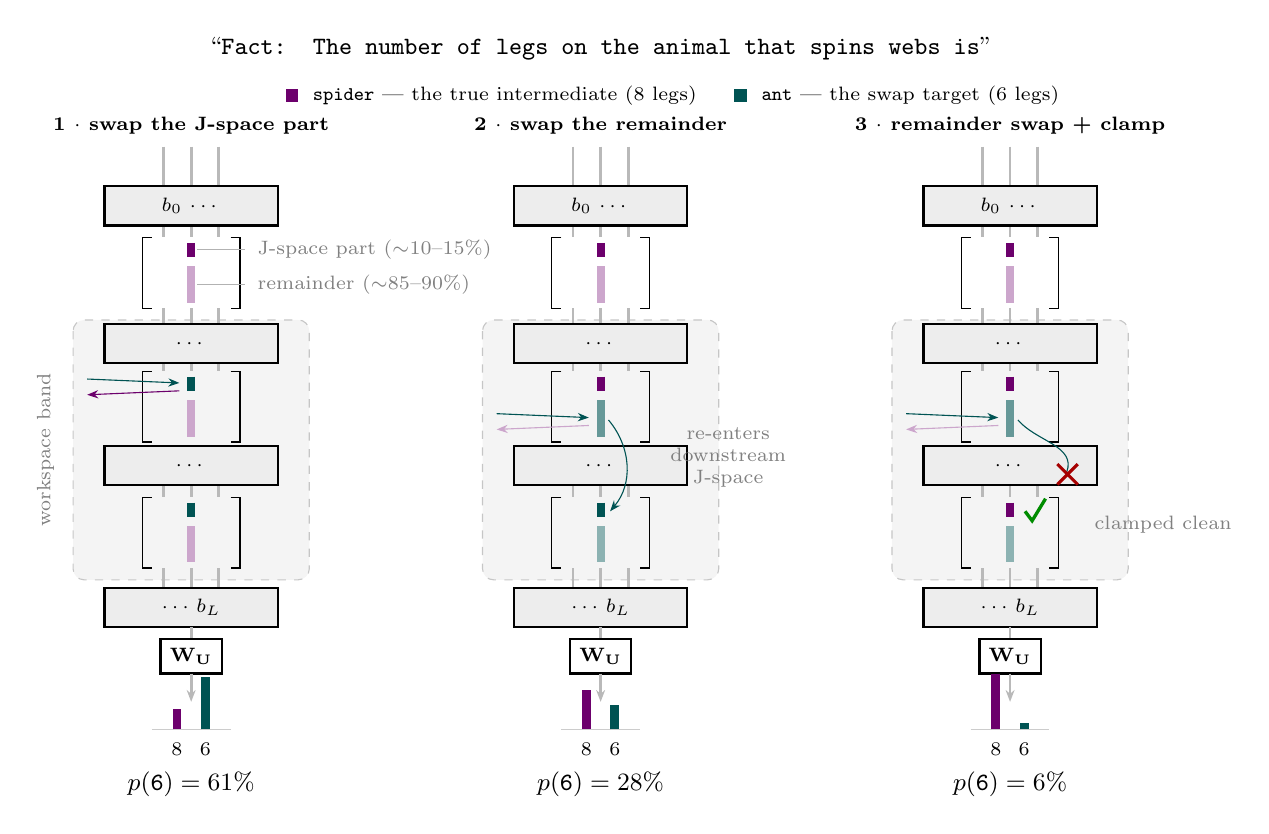
\begin{tikzpicture}
% ---- the prompt, once, at the top
\node[jlab] at (5.2,1.6) {``\texttt{Fact: The number of legs on the animal that spins webs is}''};
\fill[jvio] (1.2,0.92) rectangle +(0.16,0.16);
\node[jlabS,right] at (1.42,1.0) {\texttt{spider} --- the true intermediate (8 legs)};
\fill[jtea] (6.9,0.92) rectangle +(0.16,0.16);
\node[jlabS,right] at (7.12,1.0) {\texttt{ant} --- the swap target (6 legs)};
% ---- three panels: the common stack, then per-prong content
\foreach \PX in {0,5.2,10.4}{
\begin{scope}[xshift=\PX cm]
  % the workspace band, behind everything
  \fill[gray!9,rounded corners=4pt] (-1.5,-1.85) rectangle (1.5,-5.15);
  \draw[gray!45,dashed,rounded corners=4pt] (-1.5,-1.85) rectangle (1.5,-5.15);
  % cords (all token positions, bundled)
  \foreach \X in {-0.35,0,0.35}{
    \draw[cordJ] (\X,0.35) -- (\X,-0.15);
    \draw[cordJ] (\X,-0.65) -- (\X,-0.8);
    \draw[cordJ] (\X,-1.7) -- (\X,-1.9);
    \draw[cordJ] (\X,-2.4) -- (\X,-2.5);
    \draw[cordJ] (\X,-3.95) -- (\X,-4.1);
    \draw[cordJ] (\X,-5.0) -- (\X,-5.25);}
  % blocks
  \node[jband] at (0,-0.4) {$b_0\,\cdots$};
  \node[jband] at (0,-2.15) {$\cdots$};
  \node[jband] at (0,-3.7) {$\cdots$};
  \node[jband] at (0,-5.5) {$\cdots\,b_L$};
  \draw[cordJ] (0,-5.75) -- (0,-5.9);
  \node[draw,thick,font=\scriptsize] at (0,-6.12) {$\mathbf{W_U}$};
  \draw[cordJ,-{Stealth[length=1.5mm]}] (0,-6.34) -- (0,-6.7);
  % outcome axis + token labels
  \draw[gray!40] (-0.5,-7.05) -- (0.5,-7.05);
  \node[jlabS] at (-0.18,-7.3) {8};
  \node[jlabS] at (0.18,-7.3) {6};
\end{scope}}
% ---- panel 1: swap the J-space part
\begin{scope}
  \node[jlabS] at (0,0.62) {\textbf{1 $\cdot$ swap the J-space part}};
  \jglyph{-1.25}{jvio}{jvio!35}
  \jglyph{-2.95}{jtea}{jvio!35}
  \jglyph{-4.55}{jtea}{jvio!35}
  \draw[jtea,-{Stealth[length=1.4mm]}] (-1.32,-2.6) -- (-0.15,-2.65);
  \draw[jvio,-{Stealth[length=1.4mm]}] (-0.15,-2.75) -- (-1.32,-2.8);
  % anatomy labels, once
  \node[jlabS,gray,right] at (0.72,-0.96) {J-space part ($\sim$10--15\%)};
  \draw[gray!60,thin] (0.68,-0.96) -- (0.08,-0.96);
  \node[jlabS,gray,right] at (0.72,-1.4) {remainder ($\sim$85--90\%)};
  \draw[gray!60,thin] (0.68,-1.4) -- (0.08,-1.4);
  % band label
  \node[jlabS,gray,rotate=90] at (-1.85,-3.5) {workspace band};
  % outcome
  \draw[jvio,line width=3.2pt] (-0.18,-7.05) -- ++(0,0.26);
  \draw[jtea,line width=3.2pt] (0.18,-7.05) -- ++(0,0.67);
  \node[jlab] at (0,-7.75) {$p(\texttt{6}) = 61\%$};
\end{scope}
% ---- panel 2: swap the remainder; it re-enters downstream J-space
\begin{scope}[xshift=5.2cm]
  \node[jlabS] at (0,0.62) {\textbf{2 $\cdot$ swap the remainder}};
  \jglyph{-1.25}{jvio}{jvio!35}
  \jglyph{-2.95}{jvio}{jtea!60}
  \jglyph{-4.55}{jtea}{jtea!45}
  \draw[jtea,-{Stealth[length=1.4mm]}] (-1.32,-3.04) -- (-0.15,-3.09);
  \draw[jvio!35,-{Stealth[length=1.4mm]}] (-0.15,-3.19) -- (-1.32,-3.24);
  \draw[jtea,thin,-{Stealth[length=1.4mm]}] (0.1,-3.12) to[out=-50,in=50] (0.12,-4.28);
  \node[jlabS,gray,align=center] at (1.62,-3.6) {re-enters\\downstream\\J-space};
  \draw[jvio,line width=3.2pt] (-0.18,-7.05) -- ++(0,0.5);
  \draw[jtea,line width=3.2pt] (0.18,-7.05) -- ++(0,0.31);
  \node[jlab] at (0,-7.75) {$p(\texttt{6}) = 28\%$};
\end{scope}
% ---- panel 3: remainder swap + clamp the downstream J-space
\begin{scope}[xshift=10.4cm]
  \node[jlabS] at (0,0.62) {\textbf{3 $\cdot$ remainder swap + clamp}};
  \jglyph{-1.25}{jvio}{jvio!35}
  \jglyph{-2.95}{jvio}{jtea!60}
  \jglyph{-4.55}{jvio}{jtea!45}
  \draw[jtea,-{Stealth[length=1.4mm]}] (-1.32,-3.04) -- (-0.15,-3.09);
  \draw[jvio!35,-{Stealth[length=1.4mm]}] (-0.15,-3.19) -- (-1.32,-3.24);
  \draw[jtea,thin] (0.1,-3.12) to[out=-50,in=70] (0.72,-3.78);
  \draw[jdn,line width=1.1pt] (0.6,-3.68) -- (0.86,-3.94);
  \draw[jdn,line width=1.1pt] (0.6,-3.94) -- (0.86,-3.68);
  \draw[jgrn,line width=1.2pt] (0.19,-4.28) -- (0.28,-4.4) -- (0.45,-4.12);
  \node[jlabS,gray,right] at (0.95,-4.45) {clamped clean};
  \draw[jvio,line width=3.2pt] (-0.18,-7.05) -- ++(0,0.7);
  \draw[jtea,line width=3.2pt] (0.18,-7.05) -- ++(0,0.08);
  \node[jlab] at (0,-7.75) {$p(\texttt{6}) = 6\%$};
\end{scope}
\end{tikzpicture}}
\caption{The three-pronged swap. The probe direction for the unspoken intermediate (\texttt{spider}) splits into a J-space part---a sparse nonnegative combination of $k{=}25$ lens rows, only ${\sim}10\text{--}15\%$ of the probe's variance---and the ${\sim}85\text{--}90\%$ remainder. All interventions act at every layer of the workspace band, at every token position. \textbf{(1)} Swapping just the J-space part for \texttt{ant}'s flips the answer $61\%$ of the time. \textbf{(2)} Swapping only the remainder still works $28\%$ of the time---but only because downstream layers read the moved content and re-express it into their own J-space (teal arrow). \textbf{(3)} Same remainder swap with the downstream J-space coordinates clamped to their clean (\texttt{spider}) values: the re-entry is blocked and the effect collapses to $6\%$. The ${\sim}10\text{--}15\%$ carries the causal freight; the ${\sim}85\text{--}90\%$ moves behavior only by being re-admitted into J-space.}
\label{fig:three-prong}
\end{figure}

\subsection{Further J-vision}

Anthropic's paper showcases many more readings and interventions sanctioned by the \(\jlens\) and \(\jspace\) and, even if you skip the mechanisms, the visualizations (some of which are interactive) are an exciting delight. Additionally, they have collaborated with \textbf{Neuronpedia} to give the public extensive access to \textbf{J-vision} in LLMs on an \href{https://www.neuronpedia.org/qwen3.6-27b/jlens?shareId=cmr1qav5a0008pt2xhsvp0scq}{interactive website}. It is the most profound way to familiarize yourself with these tools short of replicating them yourself.


Finally, there are many questions that we can imagine asking with \textbf{J-glasses} affixed to our eyes. The class of research I'd most like to see or conduct involves measuring \textit{dispositional abstraction} in terms of \(\jlens\) and \(\jspace\). Abstraction is a---if not \textit{the}---foundational faculty in intelligent systems. It takes many forms and could be defined in many ways. Neural networks, at a basic level, are constructed to embody abstraction in the way they conduct sequential \textit{templatic} processing. Any row of neurons---specified by a matrix which acts on an incoming vector---is just a series of templates which score the incoming vector for its fit in each template. The point of having dot products, wrapped in nonlinear activation functions is so that many specifically-different inputs can produce the same activations within a model---i.e. the model can \textit{see} them as the same thing. This is abstraction: seeing the similar in two things that are, on their surface, different. 

As I suggest, activation vectors are meant to be abstract representations of the input (ever more so as you go deeper in the model's layers). But in LLMs, activations are only a means to an eventually verbalized end. The \(\jlens\) is exactly the object that translates internal activations to the behavioral propensities they represent. These propensities or dispositions are actually better signals for ``what the model sees as mattering" in a given input---i.e. they are better reads on the model's abstract understanding of the input, as denoted by what it is wont to say. 

I would like to see the normalized dot product alignment (mean-subtracted) of \(\jlens\) readout scores and \(\jspace\) components as compared with raw activations \(h\) in LLMs when they're given sets of prompts that ``mean or ask the same thing". Now this is not a trivial notion to define, but, for example ``\texttt{France's capital is:}" and ``\texttt{What is the capital of France?}" are asking for the same exact answer. So are ``\texttt{8 + 9 =}" and ``\texttt{When I add 8 and 9 I get: }". In these kinds of semantically identical factual questions, does \(\jlens\) or \(\jspace\) alignment outpace \(h\) alignment on the layer axis? Similar classes of prompts could be composed for summarization tasks, or, interestingly, prompts that are actually verbatim identical except for some spelling or punctuation errors. Perhaps when a question is spelled poorly as compared with a perfect baseline, the model's disposition collapses later, as earlier layers spend their time sorting out those errors. 

% NOTE TO ADDRESS (Ben) --- the compression-vs-abstraction confound, and the control that
% answers it. \jlens is a linear map with a large effective null space, so it collapses
% EVERYTHING, not just paraphrases; any projection raises apparent similarity by discarding
% variance. Showing \jlens(h_1) \approx \jlens(h_2) while h_1 \not\approx h_2 therefore proves
% compression, not abstraction, and that is the first objection a reader will raise.
% The fix is a difference-in-differences: the claim cannot be "equivalent prompts converge under
% \jlens", it has to be "equivalent prompts converge MORE THAN UNRELATED prompts do under \jlens,
% relative to that same contrast under h". Optionally add a random projection of matched rank as a
% second baseline --- if a random rank-matched projection reproduces the convergence, the effect is
% dimensional rather than semantic. Naming this control here makes the proposal look considered
% rather than naive, and it costs one or two sentences.

%% HYPOTHESIS SKETCH (no data): dispositional abstraction converging ahead of
%% representational abstraction. Reference as Figure~\ref{fig:disposition-race}.
\begin{figure}[htbp]
\centering
\resizebox{0.86\textwidth}{!}{%
\begin{tikzpicture}[x=1cm,y=1cm,
  lab/.style={font=\footnotesize},lil/.style={font=\scriptsize},
  wv/.style={line width=1.2pt}]
% ---- the pair
\node[lil,gray!70!black,anchor=west] at (-0.1,4.45) {\emph{two prompts, one answer}};
\node[draw,rounded corners=2pt,fill=gray!8,lil,anchor=west,inner sep=4pt,text width=40mm]
      at (-0.1,3.62) {``\texttt{France's capital is:}''};
\node[draw,rounded corners=2pt,fill=gray!8,lil,anchor=west,inner sep=4pt,text width=40mm]
      at (-0.1,2.70) {``\texttt{What is the capital of France?}''};
\draw[decorate,decoration={brace,mirror,amplitude=3pt},gray!60] (4.35,2.32) -- (4.35,4.00)
      node[midway,right=4pt,lil,gray!70!black,align=left]{both\\ demand\\ ``\texttt{Paris}''};
\node[lil,gray!70!black,anchor=north west,align=left,text width=52mm] at (-0.1,1.85)
      {The surface forms share almost no tokens. Does the
       \emph{disposition} they induce converge sooner than the
       \emph{representation} does?};
% ================= the plot =================
\begin{scope}[shift={(6.6,0.35)}]
\fill[gray!10] (2.45,0) rectangle (6.45,4.60);
\node[lil,gray!55] at (4.45,4.80) {workspace band};
\draw[-{Stealth[length=1.8mm]},gray!70] (0,0) -- (7.7,0)
      node[right,lil,gray!70!black]{layer depth};
\draw[-{Stealth[length=1.8mm]},gray!70] (0,0) -- (0,5.05);
\node[lil,gray!70!black,rotate=90,anchor=south] at (-0.5,2.3) {alignment across the pair};
\node[lil,gray!55,anchor=east] at (-0.12,0.06) {none};
\node[lil,gray!55,anchor=east] at (-0.12,4.45) {same};
\node[lil,gray!55,anchor=north] at (0.15,-0.14) {early};
\node[lil,gray!55,anchor=north] at (7.0,-0.14) {late};
% --- S(h): sparse support overlap --- hypothesised to converge first
\draw[wv,jvio] plot[smooth,tension=0.7] coordinates
  {(0,0.41) (0.875,0.71) (1.75,1.54) (2.625,2.87) (3.5,3.75) (4.375,4.15) (5.25,4.29) (6.125,4.34) (7,4.35)};
\node[lil,jvio,anchor=west] at (7.12,4.35) {$\jspace(h)$};
% --- L(h): the readout distribution
\draw[wv,jtea] plot[smooth,tension=0.7] coordinates
  {(0,0.44) (0.875,0.62) (1.75,1.06) (2.625,2.09) (3.5,3.12) (4.375,3.68) (5.25,3.91) (6.125,3.98) (7,4.01)};
\node[lil,jtea,anchor=west] at (7.12,3.95) {$\jlens(h)$};
% --- raw activations
\draw[wv,black!75] plot[smooth,tension=0.7] coordinates
  {(0,0.38) (0.875,0.46) (1.75,0.54) (2.625,0.69) (3.5,0.93) (4.375,1.38) (5.25,2.09) (6.125,2.94) (7,3.44)};
\node[lil,black!75,anchor=west] at (7.12,3.40) {$h$};
% --- the shape the sketch is claiming
\draw[gray!55,thin,dashed] (2.25,0) -- (2.25,2.30);
\draw[gray!55,thin,dashed] (5.45,0) -- (5.45,2.30);
\draw[{Stealth[length=1.5mm]}-{Stealth[length=1.5mm]},gray!65,thin] (2.25,0.26) -- (5.45,0.26);
\node[lil,gray!70!black,align=center] at (3.85,0.72) {disposition agrees\\ well before the states do};
\end{scope}
\end{tikzpicture}}
% CAPTION STUB (Ben to expand)
\caption{\textbf{A hypothesis, not a result---the curves are drawn, not measured.} Two prompts that
demand the same answer share little on the surface. Plotted against depth is how closely the pair
\emph{agrees} under three readings of the same activations: the raw states $h$, the \textbf{J-lens}
readout $\jlens(h)$, and the \textbf{J-space} decomposition $\jspace(h)$. The sketch states the
conjecture this section proposes---that what a model is \emph{disposed to say} about two paraphrases
converges earlier in depth than what it \emph{represents} about them, and that the sparse $\jspace$
support (do the two select the same tokens?) converges earliest of all. No axis carries units and no
curve carries data; the shape is the claim, and testing it is the point.}
\label{fig:disposition-race}
\end{figure}

These are open questions, but \textbf{J-vision} gives us the ability to ask them. 

\section{Causal Privilege}

Calculus is the language of cause. To influence a system purposefully, to understand it to the point of intervention, one must map its elements for their causal privilege. In many systems that we build from the ground up, calculus isn't needed to map cause through the system. But since neural networks are developed indirectly to the human mind, we have to rediscover the causal roots that took hold in the network using calculus.

The \textbf{J-lens} gave us the \textbf{J-space}, a causally privileged set of levers that training discovered, bootstrapped, and put to use. Through it, we begin to wrest the most vexing curse of deep learning. Ceding the manual construction of a hierarchy of causal privilege, we let backpropagation---whose perceptual field and logic of influence is calculus---deliver us a coherent system to the understanding of whose logic we held no initial claim. Stunning proficiency outran stable understanding. That we've now found this leverage and made it legible in a system that draws such due awe is an achievement to behold---an achievement that should excite us.

The \textbf{J-space} is not an end reached, but the first revelation of the internal coherence we coaxed into emergence. Endowed with too much representational and algorithmic capacity, these systems crystallized an obvious coherence---obvious by their stunning behavior, which has already marshaled trillions of dollars of attention. For such a jungle to behave so coherently, there had to have been hierarchies formed, the effective complexity had to have collapsed; local, deterministic(, ``dumb") behaviors had to be bent \textit{upward} in service of a higher level organization. This is causal emergence.\footnote{\textit{Causal emergence} is a technical notion (Hoel, Albantakis, and Tononi, 2013): a coarse-grained \textit{macro}-scale of a system can hold \textit{more} causal power---a higher \textit{effective information}---than the fine-grained \textit{micro}-scale beneath it. It is invoked here deliberately rather than as loose metaphor: the model's behavior is steered by a few macro-directions that training distilled from a vastly over-parameterized micro-substrate.} What better equipment with which to discover the causal structures we've blindly coerced than the language of cause itself?

Coloring the network with legible causal links is an old achievement. Only when the models proved to have organized hierarchically---to have allocated privilege non-uniformly on the inside as evidenced by the non-trivial success on the outside---was it time to peel the layers back and find that privilege. Random networks can be interpreted end-to-end in terms of legible cause. Only when they evidenced to have reflected our choice domain into their internal mechanism did we have---at once---the ability and \textit{obligation} to find that reflection in the form of privileged neural circuits.

% \section{Persuadability}\label{sec:persuade}

% Persuadability is the sign of an intelligent system. The thinner the causally successful intervention, the higher-level your signal, the more organization is evidenced in the system you've persuaded. To causally intervene on a [low level thing], we practically have to meet it where it is and physically reinforce it. To get the bugs away from our dinner table, we place a bright light on the edge of the patio; we did not have to touch their bodies at all, but knew that the new reality to which we subjected them would filter down into their behavior, to our predicted advantage. While predictable, the intervention doesn't stick; the bugs won't learn to avoid our table, we must put the light on every time. To predictably (and lastingly) steer the behavior of a horse, cow, or dog, we do not have to know a thing about their internal biology---we can steer them simply with food. With enough transactive communication---no words, no physical touch even necessary---



% \subsubsection*{Notes toward the argument \textnormal{\textit{(scaffolding --- shape into prose and delete; your existing prose and \% notes above are untouched)}}}

% \paragraph{The thesis, from your own text.} \textit{This is the load-bearing move, and it is stronger than the ladder alone:}
% \begin{quote}\itshape
% We already had the top level persuasion: text. We already had the low level too; intervene everywhere with exactness. Now we have something like medicine. Physical reinforcement, but semantic, understood, and trusting of internal mechanism to stably recover after our nudge. It is the middle ground between hands off trust and hands on force. We can fuck your priors and trust that you'll consequence them coherently.
% \end{quote}

% \noindent Why this earns the section its place in \textit{this} paper: it is not an appreciation of leverage in general, it is a claim about what \textbf{J-vision adds}. Prompting was always available. Weight surgery was always available. What did not exist before is a register with \textbf{direct access that is nonetheless semantic}---and that is precisely what a lens-coordinate swap is.

% \begin{itemize}\itemsep2pt
% \item \textbf{Three registers, not a spectrum of thinness.} Top: text, prompting---hands off, we ask and trust. Bottom: weights and activations edited everywhere with exactness---hands on, we force. Middle (new): intervene \textit{physically}, on the actual substrate, but in \textit{the system's own semantic vocabulary}, and let its competence carry the consequence.
% \item \textbf{The existing bugs/dog/human ladder becomes the setup, not the point.} It establishes the two poles---the light on the patio and the food in the hand are hands-off trust; nothing in that ladder touches the animal. Land the ladder on the middle register rather than on ``thin is impressive''.
% \item \textbf{Medicine is the right analogy because of \emph{why} it works.} Medicine is physical and it is semantic: it addresses the body in a language the body already regulates itself in, and it works because the body has the homeostatic competence to metabolise the intervention and re-stabilise. Same shape: the swap is a real edit to real activations, expressed in a vocabulary the network already computes in, absorbed by machinery that lands on its feet.
% \end{itemize}

% \paragraph{The guard the argument needs.} \textit{Your ``trusting of internal mechanism to stably recover after our nudge'' already supplies this---make sure it survives into the prose, because without it a reader collapses persuadability into mere sensitivity.} Leverage alone does not distinguish persuasion from chaos: a butterfly has an enormous effect-to-cause ratio and is neither steerable nor legible. Persuadability is leverage \textbf{plus predictability plus the system's self-stabilising competence}. That third term is what the swaps demonstrate and what a chaotic system lacks: the model does not merely \textit{react} to the intervention, it \textit{consequences} it coherently---answers the new question, keeps the grammar, finishes the couplet.

% \paragraph{The empirical anchors already in hand.}
% \begin{itemize}\itemsep2pt
% \item \textbf{The three-pronged swaps} (\S\ref{sec:jfindings}) --- leverage, measured: \({\sim}10\text{--}15\%\) of a probe's variance carries \({\sim}60\%\) of the behaviour, and clamping the \(\jspace\) coordinates collapses the remainder's effect to \(6\%\). A thin, semantic, upstream nudge with coherent downstream reach.
% \item \textbf{Counterfactual reflection training} (\texttt{\#reflection}) --- \textit{this is the thesis run as an experiment, by them.} They trained only the capacity to \textit{articulate} ethical principles under interruption---a purely semantic intervention---and ordinary, uninterrupted behaviour improved, with no direct training of that behaviour. Ablating the implanted representations reverted the gain. That is ``fuck your priors and trust you'll consequence them coherently,'' demonstrated.
% \item \textbf{Selectivity} (Figs.~20--21) --- the honest limit on the claim: automatic processing routes \textit{around} this channel entirely. We can persuade what the workspace touches, and not what it doesn't.
% \end{itemize}

% \paragraph{Still to decide.}
% \begin{itemize}\itemsep2pt
% \item \textbf{Define ``size'' in the leverage ratio.} It is doing heavy work in the SEED note above. Description-length or dimensionality of the intervention, against the coherent scope of the downstream change, is the reading I would pick---but pick one and name it.
% \item \textbf{``Both we and the model independently discovered it.''} Strong and lovely; ground it in the finding that downstream weights \textit{amplify} \(\jspace\) directions---the model built its own high-leverage control surface and we learned to read and push it.
% \item \textbf{Levin} is a real researcher with specific empirical claims (bioelectric goal-signals reprogramming morphology without editing the genome). Frame as resonance, not equivalence; do not imply he said anything about language models.
% \item \textbf{Coda collision.} \S\ref{jvizllm}'s whistling passage already carries the sibling idea (high-level goals filtering down through nested mechanism). Decide whether persuadability lives here, there, or bridges them---the standing risk is three overlapping endings.
% \end{itemize}


\section{The Horizons of J-vision}

As I wrote this document, I stepped out to pick up dinner and indulged in a whistle-along car ride. I am a good whistler, but tonight there was unusual accord between the sounds I wanted and those that were broadcast from my mouth. It stirred me to think about the control my brain was exerting over many distinct modules of my body. The physics of human whistling are far beyond my competency, and I know for sure its theorems and equations are etched nowhere in my brain. All that my brain needs to know to realize my conviction---which we won't bother interrogating today---is a \textbf{J-lens} differentiating \textit{whistled frequency} with respect to what I am loosely imagining as a stream of \textit{electrical command vectors} propagating from my brain to my diaphragm, lungs, throat, lips, and tongue. The algorithm does not need realization, only \(\mathbb{E} [\frac {\partial \mathbf{Pitch}}  {\partial \mathbf{Command}}]\) does (and even this quantity is not \textit{realized}, but baked into the machinery).

Why \(\mathbb{E}\)? I can whistle with similar aptitude across many different physical contexts; wet lips after a shower, dry lips on a cold winter day, laying on my back, walking on the treadmill, engaging my tongue or not, optimizing for volume or exactness...In each context, the machine to control is slightly different, but the function that describes how to change notes in any of these contexts is overwhelmingly quite similar. Whatever the realization of the whistling \textbf{J-lens} in my brain, it is an average over contexts. I can pick up whistling without having any conscious awareness of the moisture on my lips or in the air. Sure, once this information is known, there's some steering and tuning that occurs (the \textbf{J-lens} is not all-seeing, the \textbf{J-space} does not exist or act alone!), but there is a directional map of where to go in \textit{electrical command space} to reach a desired location in \textit{whistled frequency space}. 

One more feature of the whistling lens bears mentioning here, as it relates to robustness of disposition. The map from \textit{command space} to \textit{frequency space} is \textit{non-injective,} meaning it exhibits \textbf{many-to-one} relationships. There are many, many specific commands my brain can stream that will achieve the same frequency, especially when the diverse contexts above are considered. There is, then, a notion of \textit{fibers} with respect to this map. There are directions in command space that can be traversed that will not change the corresponding output in frequency space. If I want to stay on tune and remain alive, I must breathe through my performance; my brain evidently has found invariant fibers along which it should travel in command space as the periods of respiration occur. The same idea goes for the moisture of my lips, which is constantly changing, especially when I whistle. There are circuits in the brain that can pin the required invariant---pitch---with a proficient honoring of the fibers admitted under the \textbf{J-lens}. \textbf{J-vision} gives us a new intuitive vocabulary with which to explain cybernetics---in differentiable and non-differentiable machines alike. 

The mystery of how high-level mental goals filter down through mechanism into realization has always tantalized me. \textbf{J-vision} is the beginning of the answer. Anthropic's results suggested that Claude's downstream weights specifically amplify privileged \textbf{J-space} directions internally, and we have to imagine that such a privileged space (in any layer \(\ell\)) developed in concert with other parameters (in layers \(\ell' < \ell\)) that learned to exert high-leverage influence on the future behavior of the model by manifesting changes in  \(h_\ell\). But beyond a system's internal apprehension (by way of \textbf{J-vision}) of its high leverage states, we as machine learning engineers are tantalized by \textit{our own} interventional opportunities as \textit{external} agents. If the brain has modules akin to language models, we can imagine that higher-level systems have found their own levered hooks informed by \textbf{J-vision} as well that can enable executive steering. 

\textbf{J-vision} is both the generalized ability to map changes in high-leverage control variables to those in downstream domains of behavior \textit{as well as} the disposition to think about and look at hierarchical systems in this framing. \textbf{J-vision} the ethos seeks \textbf{J-vision} the practice, which fans the flames of the ethos, and so on. We've just gotten our first \textbf{J-glimpse}. 

\end{document}


